\documentclass[nobib,notoc,twoside,symmetric]{tufte-book}
\setcounter{tocdepth}{4}
\setcounter{secnumdepth}{4}

\usepackage{marginfix}
%to fix margins
\usepackage{multicol}
%for two-column.
\usepackage{CJKutf8}
%for mandarin

%\usepackage{scrextend} 
%\changefontsizes[11pt]{12pt}

\renewcommand{\footnotesize}{\small}

\geometry{a4paper,landscape,inner=30mm,top=15mm,bottom=10mm,headsep=\baselineskip,textwidth=170mm,marginparsep=8mm,marginparwidth=80mm,textheight=170mm,headheight=\baselineskip}

%\geometry{showframe}% for debugging purposes -- displays the margins

%\usepackage{stmaryrd}
%\usepackage{fontawesome}

\usepackage{amsmath,amsthm,amssymb,amsfonts}
\theoremstyle{definition}
\newtheorem{theorem}{Theorem}[section]
\newtheorem*{theorem*}{Theorem}
\newtheorem{corollary}[theorem]{Corollary}
\newtheorem{lemma}[theorem]{Lemma} 
\newtheorem{proposition}[theorem]{Proposition}
\newtheorem{conj}[theorem]{Conjecture}
\newtheorem{defn}[theorem]{Definition}
\newtheorem{fact}[theorem]{Fact} 
\newtheorem{example}[theorem]{Example} 
\newtheorem{examples}[theorem]{Examples}
\newtheorem{example*}[theorem]{Example*}
\newtheorem{examples*}[theorem]{Examples*}
\newtheorem{remark}[theorem]{Remark}
\newtheorem{remark*}[theorem]{Remark*}
\newtheorem{question}[theorem]{Question}
\newtheorem{assumption}[theorem]{Assumption}
\newtheorem{conjecture}[theorem]{Conjecture}
\newtheorem{convention}[theorem]{Convention}
\newtheorem{justification}[theorem]{Justification} 
\newtheorem{construction}[theorem]{Construction}
\newtheorem{rem}[theorem]{Reminder}
\newtheorem{intuition}[theorem]{Intuition}
\newtheorem{term}[theorem]{Terminology}
\newtheorem{scholium}[theorem]{Scholium}
\newtheorem{requirement}[theorem]{Requirement}
\newtheorem{notation}[theorem]{Notation}
\newtheorem{refinement}[theorem]{Refinement}
\newtheorem{thesis}[theorem]{Thesis}

%for fonts
\usepackage{newpxtext}
%\usepackage[fracspacing]{newpxmath}
\linespread{1.05}

\usepackage{tikz-cd}
\usepackage{macros/tikzfig}
\usepackage{macros/quiver}
\input{macros/thesis.tikzstyles}

% Set up the images/graphics package
\usepackage{graphicx}
\setkeys{Gin}{width=\linewidth,totalheight=\textheight,keepaspectratio}
\graphicspath{{graphics/}}

\title{String diagrams for text}
\author[V.W.]{Vincent Wang-Ma\'{s}cianica}
\date{\today}

% The following package makes prettier tables.  We're all about the bling!
\usepackage{booktabs}

% The units package provides nice, non-stacked fractions and better spacing
% for units.
\usepackage{units}

% The fancyvrb package lets us customize the formatting of verbatim
% environments.  We use a slightly smaller font.
\usepackage{fancyvrb}
\fvset{fontsize=\normalsize}

% Small sections of multiple columns
\usepackage{multicol}

% Squares
\usepackage{stix}

% Provides paragraphs of dummy text
\usepackage{lipsum}

% These commands are used to pretty-print LaTeX commands
\newcommand{\doccmd}[1]{\texttt{\textbackslash#1}}% command name -- adds backslash automatically
\newcommand{\docopt}[1]{\ensuremath{\langle}\textrm{\textit{#1}}\ensuremath{\rangle}}% optional command argument
\newcommand{\docarg}[1]{\textrm{\textit{#1}}}% (required) command argument
\newenvironment{docspec}{\begin{quote}\noindent}{\end{quote}}% command specification environment
\newcommand{\docenv}[1]{\textsf{#1}}% environment name
\newcommand{\docpkg}[1]{\texttt{#1}}% package name
\newcommand{\doccls}[1]{\texttt{#1}}% document class name
\newcommand{\docclsopt}[1]{\texttt{#1}}% document class option name

\usepackage{bussproofs}

\usepackage{xcolor}
\usepackage{xspace}
\def\bB{\begin{color}{blue}}
\def\bO{\begin{color}{orange}}
\def\bG{\begin{color}{green}}
\def\bM{\begin{color}{magenta}}
\def\e{\end{color}\xspace}

%For chesspieces
\usepackage{skak}

%For Brakets
\usepackage{physics}

\usepackage{xspace} 
%\usepackage{enumerate}
\usepackage{color} 
\def\bR{\begin{color}{red}}
\def\bB{\begin{color}{blue}}
\def\e{\end{color}\xspace}

%\usepackage{tocloft}
%\cftsetindents{section}{0em}{2em}
%\cftsetindents{subsection}{0em}{2em}
%\renewcommand\cfttoctitlefont{\hfill\Large\bfseries}
%\renewcommand\cftaftertoctitle{\hfill\mbox{}}

\begin{document}

\maketitle% this prints the handout title, author, and date

%\begin{fullwidth}
%\begin{multicols}{2}
\tableofcontents\marginnote{(Acknowledgements will go in a margin note here.)}
%\end{multicols}
%\end{fullwidth}

\newpage
\vfill
\begin{myboxB}
\centering
\textbf{Novel contributions:}
\begin{itemize}

\item Section \bR REF \e is a pedestrian introduction to weak $n$-category theory (via \texttt{homotopy.io}, underpinned by the theory of associative $n$-categories) from the perspective of generalising familiar string-rewrite systems to higher dimensions. The chief development of this section is a demonstration that context-free grammars and tree-adjoining grammars may be formalised in the $n$-categorical setting.

\item Section \bR REF \e spells out a generative grammar for text using an $n$-categorical signature as a rewrite system, which additionally provides a unified framework from which the Text Circuit Theorem first proved in \bR CITE \e is recovered.

\item Section \bR REF \e introduces the category \textbf{ContRel} of continuous relations. I detail the relationships (or lack thereof) of \textbf{ContRel} to its cousins \textbf{Top} and \textbf{Rel}. Though \textbf{ContRel} is constructed na\"{i}vely, its definition and an exposition of its expressivity from the monoidal perspective appears to be novel.

\item Section \bR REF \e string-diagrammatically characterises set-indexed collections of disjoint open subsets of spaces in \textbf{ContRel} as \emph{sticky spiders} -- special frobenius algebras that satisfy certain interaction relations with an idempotent. The diagrammatic outcome is that reasoning with such set-indexed collections remains as graphically intuitive as with spiders.

\item Section \bR REF \e -- with the aid of a theorem by Friedman \citep{friedman_fom_2005} -- string-diagrammatically characterises a vocabulary of linguistic topological relations in \textbf{ContRel} such as simple connectedness, touching, insideness, and rigid motion.

\item Section \bR REF \e argues for the centrality of explaining communication as a criterion for formal approaches to syntax, and explores the relationship between productive and parsing grammars as organised by a monoidal cofunctor. A diagrammatic treatment of monoidal cofunctor boxes is introduced for this purpose.

\item \bR REF \e is a standalone introduction to the mathematical setup of Montague's \emph{Universal Grammar}, aimed at modern algebraists. An outcome of this section is the placement of text circuits as a natural mathematical development in the broadly conceived programme of Montague Semantics.

\item Appendix \bR REF \e constructs a subcategory of sticky spiders in \textbf{ContRel} on the unit square that behaves as a model of \textbf{FinRel} equipped with a \emph{Turing object} -- a single object in a category with respect to which all other objects and morphisms between them may be encoded. This is of particular relevance to the linguistic phenomenon of \emph{entification} -- that essentially all grammatical categories of words and even phrases have noun-equivalents, e.g. $\texttt{to run} \simeq \texttt{running}$, $\texttt{Bob drinks} \simeq \texttt{the fact that Bob drinks}$. The presence of a Turing object in a symmetric monoidal category additionally provides a semantic model for higher-order processes of generic input type, and for \emph{lasso diagrams}.

\item In Section \bR REF \e, by parsing text as circuits (Section \bR REF \e) and using monoidal cofunctor boxes (Section \bR REF \e) to interpret those circuits in \textbf{ContRel} as iconic representations equipped with a vocabulary of lingustic-topological concepts (Section \bR REF \e), I compute some metaphors by hand.

\end{itemize}
\end{myboxB}
\vfill
\clearpage
\newpage

\setcounter{chapter}{-1}
\chapter{Context and synopsis}
There are potentially practical and theoretical benefits to a fresh mathematical take on basic linguistics. String diagrams are formal, intuitive, expressive, fun, and pretty. I review the relevant research context.
\clearpage
\newpage
\section{What this thesis is about}

\begin{marginfigure}
\centering
\[\resizebox{0.5\textwidth}{!}{\tikzfig{intro/model}}\]
\caption{Let's say that \textbf\emph{{the meaning of text is how it updates a model.}} So we start with some model of the way things are, modelled as data on a wire.}
\end{marginfigure}

\begin{marginfigure}
\centering
\[\resizebox{0.6\textwidth}{!}{\tikzfig{intro/model2}}\]
\caption{Text updates that model; like a gate updates the data on a wire.}
\end{marginfigure}

\begin{marginfigure}
\centering
\[\resizebox{0.7\textwidth}{!}{\tikzfig{intro/model3}}\]
\caption{Text is made of sentences; like a circuit is made of gates and wires.}
\end{marginfigure}

\begin{marginfigure}
\centering
\[\resizebox{0.8\textwidth}{!}{\tikzfig{intro/model4}}\]
\caption{Let's say that \textbf{\emph{The meaning of a sentence is how it updates the meanings of its parts.}} As a first approximation, let's say that the \emph{parts} of a sentence are the nouns it contains or refers to. Noun data is carried by wires. Collections of nouns are related by gates, which play the roles of verbs and adjectives.}
\end{marginfigure}

\begin{marginfigure}
\centering
\[\resizebox{0.9\textwidth}{!}{\tikzfig{intro/model5}}\]
\caption{Gates can be related by higher order gates, which play the roles of adverbs, adpositions, and conjunctions; anything that modifies the data of first order gates like verbs.}
\end{marginfigure}

\begin{marginfigure}
\centering
\[\resizebox{\textwidth}{!}{\tikzfig{intro/model6}}\]
\caption{In practice, higher order gates may be implemented as gates that modify parameters of other gates. Grammar, and \emph{function words} -- words that operate on meanings -- are in principle absorbed by the geometry of the diagram. These diagrams are natural vehicles for \emph{dynamic semantics}, broadly construed, where states are prior contexts and sentences-as-processes update prior contexts.}
\end{marginfigure}

\marginnote{
\begin{defn}[Text Circuits]
\emph{Text circuits} are made up of three ingredients:
\begin{itemize}
\item wires
\item boxes, or gates
\item boxes with holes that fit a box, or 2nd order gates
\end{itemize}
\end{defn}
}

\begin{marginfigure}
\centering
\[
\tikzfig{textcirc/nounwiresABN} 
\]
\caption{Nouns are represented by wires, each `distinct' noun having its own wire.}
\end{marginfigure}

\begin{marginfigure}
\centering
\[
\tikzfig{textcirc/ADJgate} \quad\quad\quad \tikzfig{textcirc/IVgate} \quad\quad\quad \tikzfig{textcirc/TVgate}
\]
\caption{We represent adjectives, intransitive verbs, and transitive verbs by gates acting on noun-wires. Since a transitive verb has both a subject and an object noun, that will then be two noun-wires, while adjectives and intransitive verbs only have one.}
\end{marginfigure}

\begin{marginfigure}
\centering
\[
\tikzfig{textcirc/ADVbox}
\]
\caption{Adverbs, which modify verbs, we represent as boxes with holes in them, with a number of dangling wires in the hole indicating the shape of gate expected, and these should match the input- and output-wires  of the box with the whole.}
\end{marginfigure}

\begin{marginfigure}
\centering
\[
\tikzfig{textcirc/ADPIVbox}
\]  
\caption{Similarly, adpositions also modify verbs, by moreover adding another noun-wire to the right.}
\end{marginfigure}

\begin{marginfigure}
\centering
\[
\tikzfig{textcirc/SCVbox}
\]
\caption{For verbs that take sentential complements and conjunctions, we have families of boxes to accommodate input circuits of all sizes. They add another noun-wire to the left of a circuit.}
\end{marginfigure}

\begin{marginfigure}
\centering
\[
\tikzfig{textcirc/CNJbox2}
\]
\caption{Conjunctions are boxes that take two circuits which might share labels on some wires.}
\end{marginfigure}

\begin{marginfigure}
\centering
\[
\tikzfig{textcirc/ADPIVgate}
\]
\caption{Of course filled up boxes are just gates.}
\end{marginfigure}

\begin{marginfigure}
\centering
\[
\tikzfig{textcirc/gatecompex1}  
\]
\caption{Gates compose sequentially by matching labels on some of their noun-wires and in parallel when they share no noun-wires, to give \underline{text circuits}.}
\end{marginfigure}

\begin{marginfigure}
\centering
\resizebox{\marginparwidth}{!}{\tikzfig{textcirc/circgen1}}
\caption{To summarise: composition by nesting corresponds to grammatical structure within sentences. Sentences correspond to filled gates, boxes with fixed arity correspond to first-order modifiers such as adverbs and adpositions, and boxes with variable arity correspond to sentential-level modifiers such as conjunctions and verbs with sentential complements.}
\end{marginfigure}

\begin{marginfigure}
\centering
\resizebox{0.75\marginparwidth}{!}{\tikzfig{textcirc/circgen2}}
\caption{Composition by connecting wires corresponds to identifying coreferences in discourse. We obtain the same circuit for multiple text presentations of the same content, e.g. \texttt{Sober Alice who sees drunk Bob clumsily dance laughs at him.} yields the same circuit as the text \texttt{Alice is sober. She sees Bob clumsily dance. Bob is drunk. She laughs at him.}}
\end{marginfigure}

\newthought{This thesis is about studying language using string diagrams.}

I am interested in using contemporary mathematical tools as a fresh approach to modelling some features of natural language considered as a formal object. Specifically, I am concerned with the compositional aspect of language, which I seek to model with the compositionality of string diagrams. Insofar as compositionality is the centrepiece of `knowledge of language', I share a common interest with linguists, but I will not hold myself hostage to their methods, literature, nor their concern with empirical capture. I will make all the usual simplifying assumptions that are available to theoreticians, such that an oracular machine will decide on lexical disambiguation and the appropriate parse using whatever resources it wants, so that I am left to work with lexically disambiguated words decorating some formal grammatical structure. It is with this remaining disambiguated mathematical structure that I seek to state a general framework for \emph{meaningful compositional representations of text}, in the same way we humans construct rich and interactable representations of things-going-on in our minds when we read a storybook. So if you are interested in understanding language, this thesis is an invitation to a conception of formal linguistics that's maybe worth a damn in a world where large language models exist.

\newthought{\textbf{Objection}: Isn't that reinventing the wheel?}

Yes, to an extent. I am not interested in the human language faculty \emph{per se}, so my aims differ. There are several potential practical and theoretical benefits that a fresh mathematical perspective on language enables. First, the mathematics of applied category theory allows us to unify different views of syntax, and conservatively generalise formal semantics to aspects of language that may have seemed beyond the reach of rigour, such as metaphor. Practically, the same mathematics allows us to construct interfaces between syntax/structure and semantics/implementation in such a way that we can control the former and delegate the latter by providing specifications without explicit implementation, which (for historical reasons I will explain shortly) is possibly the least-bad idea for getting at natural language understanding in computers from the bottom-up. Second, there are probably benefits to expressing linguistics in the same mathematical and diagrammatic lingua franca that can be used to represent and reason -- often soundly and completely -- about linear and affine algebra \citep{sobocinski_graphical_2015,bonchi_interacting_2017,bonchi_graphical_2019}, first order logic \citep{haydon_compositional_2020}, causal networks \citep{lorenz_causal_2023,jacobs_causal_2019}, signal flow graphs \citep{bonchi_categorical_2014}, electrical circuits \citep{boisseau_string_2022}, game theory \citep{hedges_string_2015}, petri nets \citep{baez_open_2020}, probability theory \citep{fritz_finettis_2021}, machine learning \citep{cruttwell_categorical_2022}, and quantum theory \citep{coecke_interacting_2011,coecke_picturing_2017,poor_completeness_2023}, to name a few applications. At the moment, the practical achievements of language algorithms de-emphasise the structure of language, and there is no chance of reintroducing the study of structure with dated mathematics.

\newthought{\textbf{Point of information:} What do you mean by natural language?}

Natural language is a human superpower, and the foundation of our collective achievements and mistakes as a species. By \emph{natural language} I mean a non-artificial human language that some child has grown up speaking. English is a natural language, while Esperanto and Python are constructed languages. If you are still reading then you probably know a thing or two already about natural language. Insofar as there are rules for natural languages, it is probable that like most natural language users, you obey the rules of language intuitively without knowing what they are formally; for example while you may not know what adpositions are, you know where to place words like \texttt{to}, \texttt{for}, \texttt{of} in a sentence and how to understand those sentences. At a more complex level, you understand idioms, how to read between the lines, how to flatter, insult, teach, promise, wager, and so on. There is a dismissive half-joke that "engineering is just applied physics", which we might analogise to absurdity as "law is just applied linguistics"; in its broadest possible conception, linguistics is the foundational study of everything that can possibly be expressed.

\newthought{\textbf{Point of information:} What are string diagrams?}

String diagrams are a pictorial syntax for interacting processes. They are compositional blueprints that we can give semantics to -- i.e. instantiate -- in just about any system with a notion of sequential and parallel composition of processes. In particular, this means string diagrams may be interpreted as program specifications on classical or quantum computers, or as neural net architectures. Moreover, we can devise equations between string diagrams to govern the behaviour of each process without having to spell out a bottom-up implementation, by asking processes to interact with other processes in certain ways. The mathematical foundation of string diagrams -- applied category theory -- is in short, the mathematics of compositionality.\\

Many fields of study have developed string diagrams as informal calculational aids, unaware of their common usage across disciplines and the rather new mathematics that justifies their use; everybody knows, but it isn't common knowledge. Why is that so? Because just as crustaceans independently converge to crab-like shapes within their own ecological niches by what is called \emph{carcinisation}, formal notation for formal theories of "real world" problem domains undergo "string-diagrammatisation" in similar isolation. Why is that so? Because our best formal theories of the real world treat complexity as the outcome of composing simple interacting parts; perhaps nature really works that way, or we cannot help but conceptualise in compositional terms. When one has many different processes sending information to each other via channels, it becomes tricky to keep track of all the connections using one-dimensional syntax; if there are $N$ processes, there may be on the order of $\mathcal{O}(N^2)$ connections, which quickly becomes unmanageable to write down in a line, prompting the development of indices in notation to match inputs and outputs. In time, probably by doodling a helpful line during calculation to match indices, link-ed indices become link-ing wires, and string-diagrammatisation is complete.\\

I will demonstrate how they are used in Section \ref{sec:proctheory} and define them formally in Section \ref{sec:diagdefs}. String diagrams are a heuristically natural yet mathematically formal syntax for representing complex, composite systems. I say \emph{mathematically formal} to emphasise that string diagrams are not merely heuristic tools backed by a handbook of standards decided by committee: they are unambiguous mathematical objects that you can bet your life on \citep{joyal_geometry_1991,joyal_geometry_nodate,maclane_natural_1963,lane_categories_2010,selinger_survey_2010}.

\section{\textbf{Question:} What is the practical value of studying language when Large Language Models exist?}
Large language models raise questions of existential concern for the field of linguistics. More narrowly, they demand justification as to why I am writing a thesis about theoretical approaches to basic linguistics as a computer scientist in current year. Although this thesis is pure theory, I wish to address the question of practical value early because I imagine practical people are impatient.

\newthought{Let me outline the terms and stakes.} Because the field is developing so quickly, assume that everything about LLMs is prefaced with "at the time of writing". Large Language Models are programs trained -- using a lot of data and a lot of compute time -- to predict the next word in text, computational techniques for which have evolved from Markov n-grams to transformers \citep{vaswani_attention_2017}. This sounds unimpressive, but -- in tandem with fine-tuning from human feedback in the case of chatGPT \citep{openai_chatgpt_2022} -- it is enough to tell and explain jokes \citep{bastian_google_2022}, pass the SAT \citep{teddy_teddynpc_i_2022} and score within human ranges on IQ tests \citep{thompson_gpt-35_2022}. There is an aspect of genuine scientific and historical surprise that text-prediction can do this kind of magic. On the account of \citep{mcshane_linguistics_2021}, computational linguistics began in a time when compute was too scarce to properly attempt rationalist, knowledge-based and theoretically-principled approaches to modelling language. Text-prediction as a task arose from a deliberate pursuit of "low-hanging fruit" as a productive and knowledge-lean alternative to doing nothing in an increasingly data-rich environment. Some observers \citep{church_pendulum_2011} expressed concern that all this fruit would be picked bare in a generation to force a return to knowledge-based methods, but those concerns appear now to be unfounded.\\

I'm sure there will be many further notable developments, and to be safe I won't make any claims about what machines can't do if we keep making them bigger and feed them more data or have them interact with one another in clever ways. Nonetheless there remain limitations that seem persistent for the foreseeable future, not in terms of \emph{capabilities}, but in terms of \emph{explainability and safety}. These models have a tendency to hallucinate facts and (ironically, for a computer) bad arithmetic \citep{hendrycks_measuring_2021}, and I imagine that the cycle of discovering limitations and overcoming them will continue. Despite whatever limitations exist in the state-of-the-art, it is evident to all sane observers that this is an important technology, for several reasons.

\begin{enumerate}
\item{
LLMs are a civilisational milestone technology. A force-multiplication tool for natural language -- the universal interface -- built from abundant data and compute in the information age may have comparably broad, deep, and lasting impact to the conversion of abundant chemical fuel to physical energy by steam engines in the industrial revolution.
}
\item{
LLMs represent a paradigm shift for humanity because they threaten our collective self-esteem, in a more pointed manner than losing at chess or Go to a computer; modifying a line of thinking from \citep{floridi_fourth_2014}, LLMs demonstrate that language and (the appearance of) complex thought that language facilitates is not a species-property for humans, and this stings on par with Darwin telling us we are ordinary animals like the rest, or Galileo telling us our place in the universe is unremarkable.
}
\item{
LLMs embody the latest and greatest case study of the bitter lesson \citep{sutton_bitter_2019}. The tragedy goes like this: there's a group of people who investigate language -- from syntax and semantics to pragmatics and analogies and storytelling and slang -- who treat their subject with formal rigour and have been at it for many centuries. Their role in the story of LLMs is remarkable because it doesn't exist. They were the only qualified contestants in a "let's build a general-purpose language machine" competition, and they were a no-show. Now the farce: despite the fact that all of their accumulated understanding and theories of language were left out of the process, the machine is not only built but also far exceeds anything we know how to build in a principled way out of all their hard-earned insight. That is the bitter lesson: dumb methods that use a lot of data and compute outperform clever design and principled understanding.
}
\end{enumerate}

I will note in passing that I have an ugly duckling problem, in that I am not strictly aligned with machine learning, nor linguists broadly construed, nor mathematical linguists. I am unfortunately placed in that I feel enough affinity to have defensive instincts for each camp, but I am distanced enough from each that I am sure to suffer attacks from all sides. Perhaps a more constructive metaphor than war is that I am writing in a cooperative spirit between domains, or that I am an arbitrageur of ideas between them. With that in mind, I am for the moment advocating on behalf of pen-and-paper-and-principles linguists in formulating a two-part reply to the devastating question, and I will switch sides later for balance. First a response that answers with practical values in mind, and then a response that asserts and rests upon the distinct values of linguists.

\section{\textbf{First Reply:} I don't know. Maybe explainability, maybe something else.}

\newthought{Expressing grammar as composition of processes might yield practical benefits. Moreover, we want economy, generality, and safety for language models, and we can potentially do that with few tradeoffs if we use the right framework.}

Simplified, half of the problem of learning language is learning the meaning of words. The meanings change over time and are context-dependent, and the words are always increasing in number. Encoding these meanings by hand is a sisyphean task. Data-driven learning methods are a good fit: the patterns to be learnt are complex and nebulous, and there is a lot of data. However, data-driven methods may be weaker at the second half of the problem: learning and executing the composition of meanings according to syntax. We can see just how much weaker when we consider the figures involved in 'the poverty of the stimulus'.\\

In short, this famous problem is the observation that humans learn language despite having very little training data, in comparison to the complexity of the learned structure. It is on the basis of this observation -- alongside many others surrounding language acquisition and use -- that Chomsky posits \citep{chomsky_new_2000} that language is an innate human faculty, the development of which is less like effortfully going to the gym and more like effortlessly growing arms you were meant to have. The explanation goes like this: we can explain how a complex structure like grammar gets learnt from a small amount of data if everyone shares an innate Universal Grammar with a small number of free parameters to be learned. Whether or not the intermediate mechanism is a species-property of humans, the point is that we humans get a very small amount of input data, that data interacts with the mechanism in some way, and then we know a language. So, now that there are language-entities that are human-comparable in competence, we can make a back-of-the-envelope approximation of how much work the intermediate mechanism is doing or saving by comparing the difference in how much data and compute is required for both the human and for the machine to achieve language-competence. Humans get about 1.5 megabytes of data \citep{mollica_humans_2019}, 90 billion neurons \citep{herculano-houzel_remarkable_2012}, and an adult human consumes around 500 calories per day for thinking, for let's say 20 years of language learning. Rounding all values \emph{up} to the closest order of magnitude, this comes to a cost metric of $10^{29} \ \text{bits} \times \text{joules} \times \text{neurons}$. PaLM -- an old model which is by its creators' account the first language model to be able to reason and joke purely on the basis of linguistic ability and without special training \citep{chowdhery_palm_2022,narang_pathways_2022} -- required 780 billion training tokens of natural language (let's discount the 198 gigabytes of source code training data), which we generously evaluate at a rate of 4 characters per token \citep{khan_what_2023} and 5 bits per character. The architecture has 540 billion neurons, and required 3.2 million kilowatt hours of energy for training \citep{tom_goldstein_tomgoldsteincs_training_2022}. Rounding values for the three units down \emph{down} to the nearest order of magnitude comes to a cost metric of $10^{41}$ bit-joule-neurons. Whatever the human mechanism is, it is responsible for an order of magnitude in efficiency \emph{give or take an order of magnitude of orders of magnitude}. It's possible that over time we can explain this difference away by various factors such as the efficiency of meat over minerals, separating knowledge of the world from knowledge of language, more efficient model architectures, or the development of efficient techniques to train new language models using old ones \citep{taori_rohan_stanford_2023}. One thing is clear: if it is worth hunting a fraction of a percent of improvement on a benchmark, forget your hares, a $10^{10}$ factor is a stag worth cooperating to feast on.\\

\newthought{The linguistic strategy for hunting the stag starts with what we know about how the mechanism between our ears works with language.} The good news is that the chief methodology of armchair introspection is egalitarian and democratic. The bad news is that it is also anarchistic and hard-by-proximity; we are like fish in water, and it is hard for fish to characterise the nature of water. So the happy observations are difficult to produce and easily verified, and that means there are just a few that we know of that are are unobjectionably worth taking into account. One, or \emph{the} such observation is \emph{systematicity}. Systematicity \bR CITE \e refers to when a system can (generate/process) infinitely many (inputs/outputs/expressions) using finite (means/rules/pieces) in a "consistent" (or "systematic") manner -- some tautologies require geniuses like Fodor to put into words. Like pornography, examples are easier than definitions. We know finitely many words but we can produce and understand infinitely many texts; we can make infinitely many lego sculptures out of finitely many types of pieces; we can describe infinite groups and other mathematical structures using finitely many generators and relations; in the practical domain of computers, systematicity is synonymous with programmability and expressibility.\\

The concepts of systematicity and compositionality are deeply linked, because the only way we know how to achieve systematicity in practice is composition. Frege's initial conception of compositionality \citep{frege_gottlob_selbst_1884} was borne of meditations on language, and states that a whole is the sum of its parts -- some tautologies require geniuses like Frege to put into words. Later conceptions of compositionality, the most notable deviation arising from meditations on quantum theory, are the same as the original, modulo variations on the formal definitions of parts and the method of summation \citep{coecke_compositionality_2021}. So there is our starting point: language is systematic and systematicity is the empirical surface of compositionality as far as we know, so compositionality is probably part of the solution to the problem of the stimulus, if not most of it.\\

The reasoning I report above should clarify why some folks don't think large language models have anything to do with language. The issue with purely data-driven architectures is either that we know immediately that they cannot be operating upon their inputs in a compositional way, or even if they do appear to be doing compositional things, their innards are too large and their workings too opaque to tell with confidence. Insofar as the task of learning language splits between learning meanings and learning the compositional rules of syntax that give rise to systematicity, I hope the framework I present in this thesis can be a proposal to split the cake sensibly between the two halves of the problem: meanings for the machines, compositionality for the commons. Syntax is still difficult and vast, but the rules are finite and relatively static. We can break the black-box by reexpressing syntax as the composition of smaller black-boxes. We all stand to benefit: we may give machines an easier time -- now they only have to learn the meanings of words well -- and we can have confidence that the internal representations of the machine -- their "mind's eye" -- contains something we can probe and understand.

\subsection{\textbf{Objection:} You're forgetting the bitter lesson.}

The bitter lesson is so harsh and often-enough repeated that this viewpoint is worth addressing proactively. The caveat that saves us is that the curse of expertise applies only to the object-language of the problem to be solved, not model architectures. We agree that qualitative improvements in problem-solving ability rarely if ever arise from encoding expert knowledge of the problem domain. Instead -- and we see this historically, tracking the evolutionary path for data-driven language models from markov chains to deep learning \citep{lecun_deep_2015}, RNNs \citep{rumelhart_learning_1987}, LSTMs \citep{hochreiter_long_1997}, and now transformers \citep{vaswani_attention_2017} -- these improvements come from \emph{architectural} innovations, which means altering the parts and internal interactions of a model: changing \emph{how} it thinks rather than \emph{what} it thinks, to paraphrase Sutton's original prescription. These structural changes are motivated by understandings (at varying degrees of formality) of the "geometry of the problem" \citep{bronstein_geometric_2021}. The value proposition here is that with an appropriate mathematical lingua franca for structure, composition, and interaction, we can mindfully design rather than stumble upon the "meta-methods" Sutton calls for, allowing experts to encode \emph{how} machines think and discover rather than \emph{what}. I hope to demonstrate in \bR Section \ref{} \e how importing compositional and structural understanding from linguistics to machine learning via string diagrams might allow us to cheat the bitter lesson in spirit while adhering to the letter.

\subsection{\textbf{Objection:} GOFAI? GO-F-yourself.}
 
Hostility (or at least indifference) to symbolic approaches is a stance espoused by virtually all of modern machine learning, and for good reasons. This stance is worth elaborating and steelmanning for pen-and-paper-people in the context of language. First, many linguistic phenomena are nebulous \citep{chapman_david_nebulosity_2010}: the boundary of a simile is like that of a cloud, not sharp like the boundary of a billiard ball. Second, linguistic phenomena are complex, dynamic, and multifactorial: there are so many interacting mechanisms and forces in the production and comprehension of language that even if we do have crisp mathematical models for all the constituent processes we are still left with something computationally irreducible. These two points together weakly characterise the kinds of problem domains where machine learning shines. It is just fact that LLM outputs today conform to any reasonable understanding of syntax, semantics, pragmatics, conversational implicature, and whatever else we have theorised. It is just a fact that they produce better poetry and humor than anything we could explicitly program according to our current understanding. It is almost a natural law that they will only get better from here.\\

So what good are pen-and-paper theories as far as practical applications are concerned? To borrow terms from concurrency, there is already plenty of liveness, what is needed is more safety; liveness is when the program does something good, and safety is a guarantee it won't do something bad. For example, there is ongoing work in integrating LLMs with stuctured databases for uses where facts and figures and ontologies matter; there is still a need for safeguards to prevent harmful outputs and adversarial attacks like prompt injection; while LLMs give a very convincing impression of reasoned thought, we would like to be sure if ever we decide to use such a machine for anything more than entertainment, such as assisting a caregiver in the course of healthcare decisions.\\

The good news is that symbolic-compositional theories are the right shape for safety concerns, because they can be picked apart and reasoned about. It is clear however that symbolic-compositional approaches by themselves are nowhere near achieving the kind of liveness LLMs have. Therefore, the direction of progress is synthesis.

\subsection{\textbf{Point of Information:} What is computational irreducibility?}

\emph{Computational irreducibility} \citep{wolfram_new_2002}, elsewhere called "type 2" problems \citep{marr_artificial_1977}, refers to a special kind of computational difficulty where the explanation of a system amounts to a total computational simulation of it. This is best understood by example. We have a closed-form mathematical expression to shortcut the computation of the evolution of a system of two point masses under gravity, but we have no such shortcut for the three-body problem; the best we can do is simulate the system's evolution, and an inconvenient fact is that even for very simple systems, it is possible that no amount of causal-mechanistic understanding will simplify compututational simulation.

\subsection{\textbf{Objection:} How does any of this improve capabilities?}

It's not meant to. The core value proposition for synthesis is explainable AI, which operates in a manner we can analyse, and if appropriate, constrain. For this purpose, merely knowing \emph{what} a deep-learning model is thinking is not enough\marginnote{I recount the following from \citep{sogaard_grounding_2023}, which argues that symbol-grounding is solvable from data alone, and in the process surveys the front of the symbol-grounding problem in AI: the issue of whether LLMs encode what words refer to and mean. On the account of \citep{bender_climbing_2020}, the performance of current LLMs is a form of Chinese Room \citep{searle_minds_1980} phenomenon, so no amount of linguistic competence can be evidence that LLMs solve the symbol-grounding problem. However, the available evidence appears to suggest otherwise. For example, large models converge on word embeddings for geographical place names that are isomorphic to their physical locations \citep{lietard_language_2021}. Since we know that brain activity patterns encode abstract conceptual space with the same mechanisms as they do physical spaces \citep{kriegeskorte_grid_2016}, extrapolating the ability of LLMs to encode spatially-analogical representations would in the limit suggest that LLMs encode meanings in a way isomorphic to how we do, at least for individual tokens, and so long as we take seriously some version of G\"{a}rdenfors' \citep{gardenfors_geometry_2014} thesis that meaning is encoded geometrically.}: solving symbol-grounding alone is a necessary but insufficient component. For instance, merely knowing what the weights of subnetworks of an image classification model represent does not meet our requirement of an understanding of the computations that manipulate those representations. Moreover, purely data-driven methods to control the computation may incur ethical costs \bR CITE \e, to say nothing of the potential harm that may result from a poorly safeguarded model \bR CITE \e. Add to this the ever-growing dirty laundry lists of AI models failing \bR CITE \e in inhuman ways, and the task of incorporating compositionality -- a formal understanding of \emph{how} models learn and reason -- gains urgency.\\

The investigation of the common ground between symbolic-composition and connectionism takes on, I suggest, essentially two, dual forms. The first kind uses connectionist methods to simulate symbolic-composition, which we can see the beginnings of in LLMs by examples such as chain-of-thought reasoning \citep{wei_chain--thought_2023-1} and by probing their behaviour with respect to understood symbolic models \citep{koralus_humans_2023}. The second kind is the inverse, where connectionist architectures are organised and reasoned with by symbolic-compositional means. Some examples of the first kind include implementing data structures as operations on high-dimensional vectors, taking advantage of the idiosyncrasies of linear algebra in very high dimension \citep{kanerva_computing_2019}, or work that explores how the structure of word-embeddings in latent space encode semantic relationships between tokens. Some examples of the second kind include reasoning about the capability of graph neural networks by identifying or isolating their underlying compositional structure \citep{liu_seeing_2023}, or architectures whose behaviour arises from compositional structure using neural nets as constituent parts, such as GANs \citep{goodfellow_generative_2014} and gradient boosted decision trees \citep{chen_xgboost_2016}. The work in this thesis builds upon a research programme -- DisCoCat \citep{coecke_mathematical_2010}, elaborated in \bR Section \ref{} \e -- which lies somewhere in the middle of a duality of approaches to merging connectionism and symbolic-composition. It is, to the best of my knowledge, the only approach that explicitly incorporates mathematically rigourous compositional structures from the top-down alongside data-driven learning methods from the bottom-up. Fortifying this bridge across the aisle requires a little give from both sides; I ask only that reader entertain some pretty string diagrams.

\subsection{\textbf{Objection:} Aren't string diagrams just graphs?}

\marginnote{A deeper objection here is that diagrams do not look like serious mathematics. Later I will give ample space to show how they are serious, but the reasons behind this rather common prejudice are worth elaborating. This is the wound Bourbaki has inflicted. Nicolas Bourbaki is a pseudonym for a group of French mathematicians, who wrote a highly influential series of textbooks. It is difficult to overstate their influence. The group was founded in the aftermath of the First World War, around the task of writing a comprehensive and rigourous foundations of mathematics from the ground up. The immediate \emph{raison-d'\^{e}tre} for this project was that extant texts at the time were outdated, the oral tradition and living history of mathematics in institutions of learning in France decimated by the deaths of mathematicians at war. In a broader historical context, Bourbaki was a reactionary response to the crisis in the foundations of mathematics at the beginning of the century, elicited by Russell's paradox. Accordingly, their aims were rationalist, totalitarian, and high-modernist, favouring abstraction and disdaining visualisation, in line with their contemporary artistic and musical fashions. Consequently, Bourbaki's Definition-Proposition-Theorem style of mathematical exposition is a historical aberration: a bastardisation of Euclid that eschews intuition via illustration and specificity in favour of abstraction and generality, pretending at timelessness, requiring years of initiation to effectively read and write, and remaining \emph{de rigeur} for rigour today in dry mathematics textbooks. The deeper objection arises from the supposition that serious mathematics ought to be arcane and difficult, as most mathematics exposition after Bourbaki is. The reply is that it need not be so, and that it was not always so! The Bourbaki format places emphasis and prestige upon the deductive activity that goes into proving a theorem, displacing other aspects of mathematical activity such as constructions, algorithms, and taxonomisation. These latter aspects are better suited for the nebulous subject matter of natural language, which not lend itself well to theorems, but is a happy muse for mathematical play.}

Yes and no! This point is best communicated by a mathematical koan. Consider the following game between two players, you and me. There are 9 cards labelled 1 through 9 face up on the table. We take turns taking one of the cards. The winner is whoever first has three cards in hand that sum to 15, and the game is a draw if we have taken all the cards on the table and neither of us have three cards in hand that sum to 15. I will let you go first. Can you guarantee that you won't lose? Can you spell out a winning strategy? If you have never heard this story, give it an honest minute's thought before reading on.\\

The usual response is that you don't know a winning strategy. I claim that you probably do. I claim that even a child knows how to play adeptly. I'll even wager that you have played this game before. The game is Tic-Tac-Toe, also known as Naughts-and-Crosses: it is possible to arrange the numbers 1 to 9 in a 3-by-3 magic square, such that every column, row, and diagonal sums to 15.\\

The lesson here is that choice of representations matter. In the mathematical context, representations matter because they generalise differently. On the surface, here is an example of two representations of the same platonic mathematical object. However, Tic-Tac-Toe is in the same family as Connect-4 or 5-in-a-row on an unbounded grid, while the game with numbered cards generalises to different variants of Nim. That they coincide in one instance is a fork in the path. In the same way, viewing string diagrams as "just graphs" is taking the wrong path, just as it would be true but unhelpful to consider graphs "just sets of vertices and edges". String diagrams are indeed "just" a special family of graphs, just as much as prime numbers are special integers and analytic functions are special functions. Throughout this thesis I will be re-presenting familiar and unfamiliar things in string diagrams, so I request the reader to remember the koan and keep an open mind.\\

In a broader context, representations matter for the sake of improved human-machine relations. These two representations are the same as far as a computer or a formal symbol-pusher is concerned, but they make world of difference to a human native of meatspace. We ought to swing the pendulum towards incorporating human-friendly representations in language models, so that we may audit those representations for explainability concerns. As it stands, there is something fundamentally inhuman and behavioural about treating the production of language as a string of words drawn from a probability distribution. I don't know about you, but I tend to use language to express pre-existing thoughts in my head that aren't by nature linguistic. Even if we grant that the latent space of a data-driven architecture is an analog for the space of internal mental states of a human user of language, how can we know whether the spaces are structurally analogous to the extent that human-machine partnership through the interface of natural language is safe? So here again is the possible solution: by composing architectures in the shape of language from the start, we can attempt guarantees that the latent-space representation of the machine is built up in the same way we build up a mental representation when we read a book or watch a film. I'll sketch how to approach this in \bR Section \ref{} \e.

\section{\textbf{Second Reply:} LLMs don't help us understand language; how might string diagrams help?}

Another way to deal with the devastating question of LLMs is to reject it, on the basis that using or understanding LLMs is completely different from understanding language, and language is worth understanding in its own right. To illustrate this point by a thought experiment, what would linguistics look like if it began today? LLMs would appear to us as oracles; wise, superhumanly capable at language, but inscrutable. Similarly, most people effortlessly use language without a formal understanding which they can express. So the fundamental mystery would remain unchanged. Understanding how an LLM works cannot help: to borrow a thought from \bR CITE \e, suppose you knew the insides of a mechanical calculator by heart. Does that mean you \emph{understand} arithmetic? At best, obliquely: implementing a computer for ideal arithmetic means compromises; the calculator is full of inessentialities and tricks against the constraints of physics. You would not know where the tricks begin and the essence ends. Similarly, suppose you knew every line of code and every piece of data used to train an LLM; does that mean you understand how language works? How does one delineate what is essential to language, and what is accidental? So the value proposition to establish is how string diagrams come into the picture for the linguist who is (definitionally) concerned with understanding how language works. Let's entertain one more objection from the practical reader and one objection from the theoretical reader before formulating a reply.

\subsection{\textbf{Objection:} Isn't the better theory the one with better predictions?}

Whether LLMs are even a theory of language is a best debatable. There are various criteria -- not all independent -- that are arguably necessary for something to qualify as an explanatory theory, and while LLMs satisfice (or even excel) at some, they fail at others. Empirical adequacy -- the ability of theory to account for the available empirical data and make good predictions about future observations -- is one such criterion \bR CITE \e, and here LLMs excel. In constast to the idealised and partial nature of formal theories, the nature of LLMs is that they are trained on empirical data about language that captures the friction of the real world. So, in terms of raw predictive power, we should naturally expect the LLMs to have an advantage over principled theories. They are so good at empirical capture that to some degree they automatically satisfy the related criteria of coherence -- consistency with other established linguistic theories -- and scope -- the ability to capture a wide range of phenomena. But while empirical capture is necessary for explanatory theories, it is insufficient.\\

\marginnote{To illustrate the insufficiency of empirical capture to make a theory, consider the historical case study of models of what we now call the solar system. The Ptolemaic geocentric model of the solar system was more empirically precise than the heliocentric Copernican, even though the latter was "more correct" \bR CITE \e. This should not be surprising, because Ptolemaic epicycles can overfit to approximate any observed trajectory of planets. It took until Einstein's relativity to explain the precession of perihelion of mercury, which at last aligned theoretical understanding with empirical observation. But Newton's theory of gravity was undeniably worthwhile science, even if it was empirically outperformed by its contemporaries. Consider just how divorced from reality Newton was: Aristotelian physics is actually correct on earth, where objects don't continue moving unless force is continually supplied, because friction exists. It took a radical departure from empirical concerns to the frictionless environment of space in order obtain the simplified and idealised model of gravity that is the foundation of our understanding of the solar system and beyond. The lessons as I see them are as follows. First, aimed towards some advocates of theory-free approaches, we should belay the order to evacuate linguistics departments because performance is to some degree orthogonal to understanding. In fact, the scientific route of understanding involves simplified and idealised models that ignore friction, and will necessarily suffer in performance while maturing, so one must be patient. Second, aimed towards some theoreticians, haphazard gluing together of different theories and decorating them with bells-and-whistles for the sake of fitting empirical observation is no different than adding epicycles; one must either declare a foundational or philosophical justification apart from empirical capture (which machines are better at anyway), or state outright that it's just a fun hobby. Third, while explainability studies in terms of analysing the behaviour of subnetworks is practically important, the whole approach seems fundamentally misguided; imagine an epicyclist explaining the precession of mercury's perihelion by pointing at a collection of epicycles and calling it a "distributed representation".}

There are several criteria where the adequacy of LLMs is unclear or debatable. Fruitfulness is a sociological criterion for goodness of explanatory theories, in that they should generate new predictions and lead to further discoveries and research \bR CITE \e. While they are certainly a potent catalyst for research in many fields even beyond machine learning, it is unclear for now how they relate to the subject matter of linguistics. Whether they satisfy Popper's criterion of falsifiability is as of yet not determined, because it is not settled how to go about falsifying the linguistic predictions of LLMs, or even express what the content of a theory embodied by an LLM is. The closest examples to falsifiability that come to mind are tests of LLM fallibility for reasoning and compositional phenomena \bR CITE \e, or their weakness to adversarial prompt-injections \bR CITE \e, but these weaknesses do not shed light on their linguistic competence and "understanding" directly.\\

Now the disappointments. LLMs are far from simple, and simplicity (Occam's Razor) is an ancient criterion for the goodness of explanation. Moreover, they fail at providing explanatory mechanisms \bR CITE \e, and they do not unify or subsume our prior understandings \bR CITE \e. The first two points are unobjectionable, so I will briefly elaborate on the criterion of unification and subsumption of prior understandings, borrowing a framework from cognitive neuroscience. A common methodology for investigating cognitive systems is Marr's 3 levels \bR CITE \e (poorly named, since they are not hierarchical, but more like interacting domains.) Level 1 is the computational theory, an extensional perspective that concerns tasks and functions: at this level on asks what the contents and aims of a system are, to evaluate what the system is computing and why, respectively. Level 2 is representation and algorithm, an intensional perspective that concerns the representational format of the contents within the system, and the procedures by which they are manipulated to arrive at outcomes and outputs. Level 3 is hardware, which concerns the mechanical execution of the system, as gears in a mechanical calculutor or as values, reads, and writes in computer memory. To be fair, in the case of LLMs, we understand well the nature of computational theory level, at least in their current incarnation as next-token-predictors, which is a narrow and clear task. Furthermore, we understand the hardware level well, from the silicon going up through the ladder of abstraction to software libraries and the componentwise activity of neural nets. There is something deeply wrong about our understanding -- if we can call it that -- of level 2. We have working understandings of several aspects about this level. We know something about the nature of internal representations in neural nets both in terms of semantic encoding within weight distributions \bR CITE \e and of token-embeddings in latent space \bR CITE \e. We can explain how transformer models work in terms of attention mechanisms and lookback \bR CITE \e, which serves as working understanding of the procedural aspect of LLMs. We also understand mathematically how it is that these models are trained using data to produce the outputs they do. The deep problem is that in spite of these understandings which should jointly cover all of level 2, we only obtain explanations at the wrong level of abstraction for the purposes we care about \bR CITE \e. Level 2 is in a sense the important level to get right for the purposes of explainability, auditability, and extension, since it is at the level of representation and procedure that we can investigate internal structure and match levels of abstraction across domains. Since the three levels interact, the challenge is to slot in a story about level 2 that coheres with what we already know about levels 1 and 3. I claim that we can go about this challenge using string diagrams as a lingua franca for mathematical linguists and machines.

\subsection{\textbf{Objection:} What's wrong with $\lambda$-calculus and sequent calculi and graphs?}

There is nothing wrong with punchcard machines either, as far as computability is concerned. String diagrams, and applied category theory more broadly, are a good metalanguage for formal linguistics. The usual choice of set theory is not well-suited for complex and interacting moving parts. The chief drawback is that set theory requires bottom-up specifications, so for instance if one wishes to specify a function, one has to spell out how it behaves on the domain and codomain, which means spelling out what the innards of the domain and codomain are; to specify a set theoretic model necessitates providing complete detail of how every part looks on the inside\footnote{This is an innate feature of set theory. Consider the case of the cartesian product of sets, one of the basic constructions. $A \times B$ is the "set of ordered pairs" $(a,b)$ of elements from the respective sets, but there are many ways of encoding ordered pairs that are equivalent in spirit but not in syntax; a sign that the syntax is a hindrance, or obfuscating something important. What we really want of the product is the property that $(a,b) = (c,d)$ just when $a = c$ and $b = d$. Now here is a small sampling of different ways to encode an ordered pair. Kuratowski's definition is
\[A \times B := \bigg\{ \{\{a\},\{a,b\}\} \ | \ a \in A \ , \ b \in B \bigg\}\]
Which could have just as easily been:
\[A \times B := \bigg\{ \{\{a,b\},b\} \ | \ a \in A \ , \ b \in B \bigg\}\]
And here is Wiener's definition:
\[A \times B := \bigg\{ \{\{a,\varnothing\},b\} \ | \ a \in A \ , \ b \in B \bigg\}\]}. As you may already know, this representation-dependency is a bureaucratic nightmare when dealing with a complex system. This leads to at least three problems.
\begin{enumerate}
\item{
The sociological problem is that this makes things difficult to understand unless you have invested a lot of time into mathematics in general.
}
\item{
Interoperability is tricky. When a programmer wants to use a data structure or algorithm, they do not always write it from scratch or copy code from stackoverflow or get their LLM to do it for them; they may use a library that provides them structures and methods they can call without worrying about how those structures and methods are implemented all the way down. However, if you building a complex theory by spelling out implementations set-theoretically from the start, incorporating a new module from elsewhere becomes difficult if that module has encoded things in sets differently. A lot of busywork goes into translating foundations of formalisms at an analogous level to machine code, which is time better spent building upwards and outwards. A computer scientist might say that some abstraction is needed, and being one, I say so.
}
\item{
Third, and related to the second, is that set-theory is not the native language for the vast majority of practical computation. Often in the design of complex theories, we do not care about how precisely representations are implemented, instead we only care about placing constraints or guarantees on the behaviour of interactions -- that is, we care about operational semantics.
}
\end{enumerate}

The problems I have mentioned above are obstacles, and I hope to show that using applied category theory as a metalanguage may be a solution. A broad theme of this thesis is to illustrate the economy and reach of applied category theory for dealing with compositional phenomena. Our capacity for language is one of the oldest and sophisticated pieces of compositional technology, maybe even the foundation of compositional thought. So, linguists are veteran students of compositionality and modularity. How does syntax compose meaning? How do the constraints and affordances of language interact? The discipline embodies a encyclopaedic record of how compositionality works "in the field", just as botanists record flowers, early astronomers the planetary motions, or stamp collectors stamps. But a disparate collection of observations encoded in different formats does not a theory make; we will inevitably wish to bring it all together. I show that we can progress towards this aim using formal diagrams that our visual cortexes have built-in rules to manipulate, and that allow us to work at the level of abstraction we choose, so that we may easily incorporate other modules and find implementations in a variety of settings.

To summarise the first value proposition, string diagrams are an aesthetic, intuitive, flexible, and rigourous metalanguage syntax that gives agency to the modeller by operating at a level of abstraction of their choice.  In this vein, theories of syntax expressed in terms of string diagrams makes it easier to reason about expressive equivalence between theories at a compositional level. More precisely, a theory of syntax is expressed as a finitely presented symmetric monoidal category, and relationships between theories are expressed as symmetric monoidal functors, which are generalised structure-preserving maps. The upshot of reasoning in this way is that equivalences are established at a structural level between the atomic components of corresponding theories, which lets us push the boundaries of what may be considered formal semantics in \bR Section \ref{} \e.

\newthought{TL;DR of introduction:} LLMs do not explain language, and formal linguists "explain" language using the mathematical equivalent of punchcard machines. Both sides stand to gain from synthesis, but synthesis requires a shared mathematical metalanguage. I propose string diagrams and applied category theory as a candidate, and the rest of the thesis is about justifying the proposal.

\section{Synopsis of the thesis}

\marginnote{
\textbf{Novel contributions:}
\begin{itemize}
\item
Section \ref{} demonstrates how string-diagrammatic reasoning allows for graphical proofs of strong equivalences between typelogical, string-production, and further strong equivalence to a fragment of tree-adjoining grammars. 
\item
Text diagrams and text circuits lie at the heart of the above correspondences and of this thesis, which we introduce and investigate in Section \ref{} in an abridged re-presentation of \bR CITE \e, culminating in a proof relating the expressive capacity of text circuits to a controlled fragment of English that serves as evidence that text circuits are a natural metalanguage for grammatical relationships that make no extraneous distinctions.
\item
In Section \ref{}, moving towards applications, I introduce the category of continuous relations, to set a mathematical stage upon which we can build toy models, expanding upon my previous work on linguistically compositional spatial relations \bR CITE \e towards modelling mechanical systems and containers.
\item
I mathematically investigate the possibilities and limitations of textual modelling with text circuits on classical and quantum computers in Section \ref{} by examining the limitations of cartesian monoidal categories for modelling text circuits, taking the universal approximation theorem into account.
\item
In Section \ref{}, I extend the string-diagrammatic techniques used to prove correspondences between different syntactic theories to text circuits provides a framework for the formal, conceptually-compliant modelling of textual metaphor.
\item
I demonstrate a formal connection between tame topologies and tensed language in Section \ref{}, which extends to a formal framework to model narratives as database rewrites in Section \ref{}.
\end{itemize}
}

Chapter 2 provides the relevant background and foundations for category theory, machine learning, and formal syntax for this thesis, which lives at the intersection. The ideas required from the parent fields will be basic, so the exposition is meant to get readers across disciplines on the same page, not impress experts. For string diagrams I will first provide a primer for how process-theoretic reasoning with string diagrams work, by example. On the category theoretic end, I will recount symmetric monoidal categories as the mathematical objects that string diagrams are syntax for, as well as provide a working understanding of PROPs \bR CITE \e and n-categories as formalised by \bR CITE \e, which provide a metalanguage for specifying families of string diagrams. Once the reader is happy with string diagrams, for machine learning I will just introduce how deep neural nets and backpropagation work in string-diagrammatic terms to provide a foundation of formal understanding, and I will explain the mathematical and real-world reasons why deep learning is so powerful. For formal linguistics, I will sketch out a partial history of categorial linguistics in general, along the way briefly recasting \bR CITE \e in more modern mathematical terminology to justify string diagrams as a generalisation of Montague's original conception of syntax and semantics.\\

Chapter 3 is about string diagrams for formal syntax. Here I recount context-free, pregroup, and tree-adjoining grammars to the reader, recast them string-diagrammatically, and relate them by means of discrete monoidal fibrations, a piece of mathematics I will develop. Then we (re)introduce text circuits as the common structure between those different theories of grammar that abstracts away differences in linear syntactic presentation while conserving a core set of grammatical relations. During my DPhil, I wrote a paper \bR CITE \e in collaboration with Jonathon Liu and Bob Coecke which introduced text circuits in a pedestrian way, and characterised their expressive capacity with respect to a controlled fragment of English. I will just recover the main beats of that paper, this time using the metalanguage of n-categories.\\

Chapter 4 sets a mathematical stage for us to model and calculate using text circuits, for which purpose I introduce the category of continuous relations \textbf{ContRel}, a na\"{i}ve generalisation of the category of continuous maps between topological spaces. \textbf{ContRel} is new, in the sense that the category-theoretically obvious approaches to obtaining such a category either do not work or yield something different. This section culminates in formal semantics for topological concepts such as \texttt{inside} which underpin the kinds of schematic doodle cartoons we might draw on paper to illustrate events occurring in space.\\

Chapter 5 is a formal invitation to playtime for the reader who gets that far. I don't expect that I've explored any novel linguistic phenomena, and I don't think I've invented any substantially new mathematics. All I've done is a form of intellectual arbitrage, putting tools from one field to work in another. To properly give weight to my claim that string diagrams and category theory are a good metalanguage for linguistics as a whole, it is necessary to demonstrate breadth. So, I model linguistic topological concepts; I give a mathematical setting for the study of generalised anaphora that reference any meaningful part of text; I provide formal semantics for the container metaphor in particular and textual metaphors in general; I sketch a formal correspondence between tensed language and tame topologies that extends to formally reckoning with narrative structure. All of this is to show that the methods I use are flexible and not doctrinal. I am not interested in whether these topics have been mathematicised more thoroughly and deeply before; what I care to demonstrate is that a little category theory and some imagination can go a long way.\\

Finally, I close with a discussion and prospectus. For the convenience of the reader, bibliographies are placed at the end of each chapter. Corrections, comments, and suggestions are welcome at \texttt{vincentwangsemailaddress@gmail.com}. I hope you enjoy the read, or if nothing else, I hope you like my diagrams!

\newpage
\section{Process Theories}

This section seeks to give an introduction to process theories in an intuitively grounded manner. We aim here to build the process-theoretic mathematics towards linguistic spatial relations -- words like "to the left of" and "between" -- which are a common ground of competence we all possess. Here we only focus on geometric relations in two dimensional Euclidean space equipped with notions of metric and distance. This section provides adequate foundations to follow \citep{}talkspace, in which I demonstrate how text circuits can be obtained from sentences and how such text circuits interpreted in the category of sets and relations \textbf{Rel} provides a semantics for such sentences. Moreover, this section motivates the question of how to express the (arguably more primitive \citep{}piaget) linguistic topological concepts -- such as "touching" and "inside" -- the mathematics of which will be in Chapter \ref{}; the reader may skip straight to that chapter after this section if they are uninterested in syntax. We close this section with a brief aside on how process theories relate to mathematical foundations and computer science.

A \emph{process} is something that transforms some number of input system types to some number of output system types. We depict systems as wires, labelled with their type, and processes as boxes. We read processes from left to right.
\[\tikzfig{proctheory/process}\]
Processes may compose in parallel, which we depict as vertically stacking boxes.
\[\tikzfig{proctheory/processpar}\]
Processes may compose sequentially, which we depict as connecting wires of the same type from left to right.
\[\tikzfig{proctheory/processseq}\]
In these diagrams only input-output connectivity matters: so we may twist wires and slide boxes along wires to obtain different diagrams that still refer to the same process. So the diagram below is equal to the diagram above.
\[\tikzfig{proctheory/processeq}\]
Some processes have no inputs; we call these \emph{states}. 
\[\tikzfig{proctheory/state}\]
Some processes have no outputs; we call these \emph{tests}.
\[\tikzfig{proctheory/test}\]
A process with no inputs and no outputs is a \emph{number}; the number tells us the outcome of applying tests to a composite of states modified by processes.
\[\tikzfig{proctheory/number}\]

A process theory is given by the following data\footnote{Formally, process theories are symmetric monoidal categories []; see section \ref{}.}:
\begin{itemize}
    \item A collection of systems
    \item A collection of processes along with their input and output systems
    \item A methodology to compose systems and processes sequentially and in parallel, and a specification of the unit of parallel composition.
    \item A collection of equations between composite processes
\end{itemize}

\begin{example}[Linear maps with direct sum]
Systems are finite-dimensional vector spaces over $\mathbb{R}$. Processes are linear maps, expressed as matrices with entries in $\mathbb{R}$.\\
Sequential composition is matrix multiplication. Parallel composition of systems is the direct sum of vector spaces $\oplus$. The parallel composition of matrices $\mathbf{A}, \mathbf{B}$ is the block-diagonal matrix
$$\begin{bmatrix}
\mathbf{A} & \mathbf{0} \\
\mathbf{0} & \mathbf{B}
\end{bmatrix}$$
The unit of parallel composition is the singleton 0-dimensional vector space.
States are row vectors. Tests are column vectors. The numbers are $\mathbb{R}$.\footnote{Usually the monoidal product is written with the symbol $\otimes$, which denotes hadamard product for linear maps. The process theory we have just described takes the direct sum $\oplus$ to be the monoidal product. To avoid confusion we will use the linear algebraic notation when linear algebra is concerned.}
\end{example}

\begin{example}[Sets and functions with cartesian product]
Systems are sets $A,B$. Processes are functions between sets $f: A \rightarrow B$. Sequential composition is function composition. Parallel composition of systems is the cartesian product of sets: the set of ordered pairs of two sets.
\[A \otimes B = A \times B := \{(a,b) \ | \ a \in A, b \in B\}\]
The parallel composition $f \otimes g : A \times C \rightarrow B \times D$ of functions $f: A \rightarrow B$ and $g: C \rightarrow D$ is defined:
\[f \otimes g := (a,c) \mapsto (f(a),g(c))\]
The unit of parallel composition is the\footnote{There are many singletons, but this presents no problem for the later formal definition because they are all equivalent up to unique isomorphism.} singleton set $\{\star\}$. States of a set $A$ correspond to elements $a \in A$\footnote{We forgo the usual categorical definition of points from the terminal object in favour of generalised points from the monoidal perspective.}. Every system $A$ has only one test $a \mapsto \star$\footnote{This is since the singleton is terminal in \textbf{Set}.}. There is only one number.
\end{example}

\begin{example}[Sets and relations with cartesian product]
Systems are sets $A,B$. Processes are relations between sets $\Phi \subseteq A \times B$, which we may write in either direction $\Phi^*: A \nrightarrow B$ or $\Phi_*: B \nrightarrow A$.\footnote{Relations between sets are equivalently matrices with entries from the boolean semiring. Relation composition is matrix multiplication with the boolean semiring. $\Phi^*,\Phi_*$ are the transposes of one another.}
Sequential composition is relation composition:
\[A \overset{\Phi}{\nrightarrow} B \overset{\Psi}{\nrightarrow} C := \{(a,c) \ | \  a \in A, \ c \in C, \ \exists b_{\in B}: (a,b) \in \Phi \wedge (b,c) \in \Psi  \}\]
Parallel composition of systems is the cartesian product of sets. The parallel composition of relations $A \otimes C \overset{\Phi \otimes \Psi}{\nrightarrow} B \otimes D$ of relations $A \overset{\Phi}{\nrightarrow} B$ and $C \overset{\Psi}{\nrightarrow} D$ is defined:
\[\Phi \otimes \Psi := \{\big( (a,c) , (b,d) \big) \ | \ (a,b) \in \Phi \wedge (c,d) \in \Psi\}\]
The unit of parallel composition is the singleton. States of a set $A$ are subsets of $A$. Tests of a set $A$ are also subsets of $A$.
\end{example}

\subsection{What does it mean to copy and delete?}

Now we discuss how we might define the properties and behaviour of processes by positing equations between diagrams. Let's begin simply with two intuitive processes \emph{copy} and \emph{delete}:
\[\tikzfig{proctheory/copydelete}\]

\begin{example}[Linear maps]
Consider a vector space $\mathbf{V}$, which we assume includes a choice of basis. The copy map is the rectangular matrix made of two identity matrices:
\[\Delta_\mathbf{V}: \mathbf{V} \rightarrow \mathbf{V} \oplus \mathbf{V} := \begin{bmatrix} \mathbf{1}_\mathbf{V} & \mathbf{1}_\mathbf{V} \end{bmatrix}\]
The delete map is the column vector of 1s:
\[\epsilon_\mathbf{V}: \mathbf{V} \rightarrow \mathbf{0} := \begin{bmatrix} 1 \\ \vdots \\ 1 \end{bmatrix}\]
\end{example}

\begin{example}[Sets and functions]
Consider a set $A$. The copy function is defined:
\[\Delta_A : A \rightarrow A \times A := a \mapsto (a,a)\]
The delete funtion is defined:
\[\epsilon_A : A \rightarrow \{\star\} := a \mapsto \star\]
\end{example}

\begin{example}[Sets and relations]\label{relcopy}
Consider a set $A$. The copy relation is defined:
\[\Delta_A : A \nrightarrow A \times A := \{\big(a , (a,a) \big) \ | \ a \in A\}\]
The delete relation is defined:
\[\epsilon_A : A \nrightarrow \{\star\} := \{(a,\star) \ | \ a \in A\}\]
\end{example}

We may verify that, no matter the concrete interpretation of the diagram in terms of linear maps, functions or relations copy and delete satisfy the equations in the margin:\marginnote[-10cm]{
Formally, the following equations characterise a cocommutative comonoid internal to a monoidal category.
\begin{equation}\label{cocom}
\scalebox{0.75}{\tikzfig{bestiary/basicrelations}}
\end{equation}
}

It is worth pausing here to think about how one might characterise the process of copying in words; it is challenging to do so for such an intuitive process. The diagrammatic equations in the margin, when translated into prose, provide an answer.
\begin{description}
\item[\textbf{Coassociativity}:] says there is no difference between copying copies.
\item[\textbf{Cocommutativity}:] says there is no difference between the outputs of a copy process.
\item[\textbf{Counitality}:] says that if a copy is made and one of the copies is deleted, the remaining copy is the same as the original.
\end{description}

Insofar as we think this is an acceptable characterisation of copying, rather than specify concretely what a copy and delete does for each system $X$ we encounter, we can instead posit that so long as we have processes $\Delta_X: X \otimes X \rightarrow X$ and $\epsilon_X: X \rightarrow I$ that obey all the equational constraints above, $\Delta_X$ and $\epsilon_X$ are as good as a copy and delete.

\marginnote{
\begin{example}[Not all states are copyable]\label{ex:copyablestate}
Call a state \emph{copyable} when it satisfies the following diagrammatic equation:
\[\tikzfig{proctheory/copyable}\]
In the process theory of sets and functions, all states are copyable. Not all states are copyable in the process theories of sets and relations and of linear maps. For example, consider the two element set $\mathbb{B} := \{0,1\}$, and let $\top : \{\star\} \nrightarrow \mathbb{B} := \{(\star,0),(\star,1)\} \simeq \{0,1\}$. Consider the composite of $\top$ with the copy relation:
\[\top;\Delta_{\mathbb{B}} := \{\big(\star,(0,0)\big),\big(\star,(1,1)\big)\} \simeq \{(0,0),(1,1)\}\]
This is a perfectly correlated bipartite state, and it is not equal to $\{0,1\} \times \{0,1\}$, so $\top$ is not copyable.
\end{example}
}
\marginnote{
\begin{remark}\label{ft:determinism}
The copyability of states is a special case of a more general form of interaction with the copy relation:
\[\scalebox{0.75}{\tikzfig{proctheory/copyablefunc}}\]
A cyan map that satisfies this equation is said to be a homomorphism with respect to the commutative comonoid. In the process theory of relations, those relations that satisfy this equation are precisely the functions; in other words, this diagrammatic equation expresses \emph{determinism}.
\end{remark}}

Here is an unexpected consequence. Suppose we insist that \emph{to copy} in principle also implies the ability to copy \emph{anything} -- arbitrary states. From Example \ref{ex:copyablestate} and Remark \ref{ft:determinism}, we know that this demand is incompatible with certain process theories. In particular, this demand would constrain a process theory of sets and relations to a subtheory of sets and functions. The moral here is that process theories are flexible enough to meet ontological needs. A classical computer scientist who works with perfectly copyable data and processes might demand universal copying along with Equations \ref{cocom}, whereas a quantum physicist who wishes to distinguish between copyable classical data and non-copyable quantum data might taxonomise copy and delete as a special case of a more generic quasi-copy and quasi-delete that only satisfies equations \ref{cocom}.\footnote{Quantum physicists \emph{do} do this; see Dodo: []}

\subsection{What is an update?}\label{ss:update}

In the previous section we have seen how we can start with concrete examples of copying in distinct process theories, and obtain a generic characterisation of copying by finding diagrammatic equations copying satisfies in each concrete case. In this section, we show how to go in the opposite direction: we start by positing diagrammatic equations that characterise the operational behaviour of a particular process -- such as \emph{updating} -- and it will turn out that any concrete process that satisfies the equational constraints we set out will \emph{by our own definition} be an update.\\

Perhaps the most familiar setting for an update is a database. In a database, an \bM entry\e often takes the form of pairs of \bB fields\e and \bO values\e. For example, where a database contains information about employees, a typical entry might look like:
\[\texttt{\bM < \bB\textbf{NAME}\e:\bO Jono Doe\e, \bB\textbf{AGE}\e:\bO 69\e, \bB\textbf{JOB}\e:\bO CONTENT CREATOR\e, \bB\textbf{SALARY}\e:\bO\$420\e, ... >\e}\]
There are all kinds of reasons one might wish to update the value of a field: Jono might legally change their name, a year might pass and Jono's age must be incremented, Jono might be promoted or demoted or get a raise and so on. It was the concern of database theorists to formalise and axiomatise the notion of updating the value of a field -- \emph{independently of the specific programming language implementation of a database} -- so that they had reasoning tools to ensure program correctness []. The problem is reducible to axiomatising a \emph{rewrite}: we can think of updating a value as first calculating the new value, then \emph{putting} the new value in place of the old. Since often the new value depends in some way on the old value, we also need a procedure to \emph{get} the current value.\\

That was a flash-prehistory of \emph{bidirectional transformations} []. Following the monoidal generalisation of lenses in [], a rewrite as we have described above is specified by system diagrammatic equations in the margin, each of which we introduce in prose.

\marginnote[-5cm]{
\begin{description}
\item[\textbf{PutPut}:] Putting in one value and then a second is the same as deleting the first value and just putting in the second.
\[\scalebox{0.5}{\tikzfig{proctheory/putputs}}\]
\item[\textbf{GetPut}:] Getting a value from a field and putting it back in is the same as not doing anything.
\[\scalebox{0.5}{\tikzfig{proctheory/getput}}\]
\item[\textbf{PutGet}:] Putting in a value and getting a value from the field is the same as first copying the value, putting in one copy and keeping the second.
\[\scalebox{0.5}{\tikzfig{proctheory/putget}}\]
\item[\textbf{GetGet}:] Getting a value from a field twice is the same as getting the value once and copying it.
\[\scalebox{0.5}{\tikzfig{proctheory/getget}}\]
\end{description}
}

These diagrammatic equations do two things. First, they completely specify what it means to get and put values in a field in an implementation independent manner; it doesn't matter whether database entries are encoded as bitstrings, qubits, slips or paper or anything else, what matters is the interaction of get and put. Second, the diagrammatic equations give us the right to call our processes \emph{get} and \emph{put} in the first place: we define what it means to get and put by outlining the mutual interactions of get, put, copy, and delete. These two points are worth condensing and rephrasing:
\[
\textbf{A \emph{kind of process} is determined by patterns of interaction with other kinds of processes.}
\]

Now we can diagrammatically depict the process of updating Jono's age, by \bB getting\e Jono's \bO age value\e from their \bM entry\e, incrementing it by 1, and \bB putting\e it back in.

\[\tikzfig{proctheory/incrementage}\]

\subsection{Spatial predicates}

The following simple inference is what we will try to capture process-theoretically:

\begin{itemize}
\item \texttt{Oxford is north of London}
\item \texttt{Vincent is in Oxford}
\item \texttt{Rocco is in London}
\end{itemize}

How might it follow that \texttt{Rocco is south of Vincent}?\\

One way we might approach such a problem computationally is to assign a global coordinate system, for instance interpreting `north' and `south' and `is in' using longitude and latitude. Another coordinate system we might use is a locally flat map of England. The fact that either coordinate system would work is a sign that there is a degree of implementation-independence.\\

This coordinate/implementation-independence is true of most spatial language: we specify locations only by relative positions to other landmarks or things in space, rather than by means of a coordinate system. This is necessarily so for the communication of spatial information between agents who may have very different reference frames.\\

So the process-theoretic modelling aim is to specify how relations between entities can be \emph{updated} and \emph{classified} without requiring individual spatial entities to intrinsically possess meaningful or determinate spatial location.\\

So far we have established how to update properties of individual entities. We can build on what we have so far by observing that a relation between two entities can be considered a property of the pair.

\[placeholder\]

Spatial relations obey certain compositional constraints, such as transitivity in the case of `north of':

\[placeholder\]

Or the equivalence between 'north of' and 'south of' up to swapping the order of arguments:

\[\]

There are other general constraints on spatial relations, such as order-independence: the order in which spatial relations are updated does not (at least for perfect reasoners) affect the resultant presentation. This is depicted diagrammatically as commuting gates:

\[placeholder\]

\subsection{Processes, Sets, Computers}

\newthought{\texttt{Objection:} But what are the \emph{things} that the processes operate on?}

This is a common objection from philosophers who want their ontologies tidy. The claim roughly goes that you can't really reason about processes without knowing the underlying objects that participate on those processes, and since set theory is the only way we know how to spell out objects intensionally in this way, we should stick to sets. In simpler terms, if we're drawing only functions as (black)-boxes in our diagrams, how will we know what they do to the elements of the underlying sets?\\

The short answer is that -- perhaps surprisingly -- reasoning process-theoretically is mathematically equivalent to reasoning about sets and elements for all practical purposes; it is as if whatever is going on \emph{out there} is indifferent to whether we describe using a language of only nouns or only verbs.\\

In the case of set theory, let's suppose that instead of encoding functions as sets, we treat functions as primitive, so that we have a process theory where wires are labelled with sets, and functions are process boxes that we draw. The problem we face now is that it is not immediately clear how we would access the elements of any set using only the diagrammatic language. The solution is the observation that the elements $\{x \ | \ X\}$ of a set $X$ are in bijective correspondence with the functions from a singleton into $X$: $\{ f(\star) \mapsto x \ | \ \{\star\} \overset{f}{\rightarrow} X $. In prose, for any element $x$ in a set $X$, we can find a function that behaves as a pointer to that element $\{\star\} \rightarrow X$. So the states we have been drawing, when interpreted in the category of sets and function, are precisely elements of the sets that label their output wires.\\

The full and formal answer will require the reader to see Section \ref{} which spells out the category theory underpinning process theories. The caveat here is that process theories work for all \emph{practical} purposes, so I make no promises about how diagrams work for the kind of set theories that deals with hierarchies of infinities that set theorists do. For other issues concerning for instance the set of all functions between two sets, that requires symmetric monoidal closure, for which there exist string-diagrammatic formalisms \citep{}.

\newthought{\texttt{Objection:} But if they're expressively the same, what's the point?}

The following rebuttal draws on Harold Abelson's introductory lecture to computer science \citep{} (in which string diagrams appear to introduce programs without being explicitly named as such).\\

There is a distinction between declarative and imperative knowledge. Declarative knowledge is \emph{knowing-that}, for example, 6 is the square root of 36, which we might write $6 = \sqrt{36}$. Imperative knowledge is \emph{knowing-how}, for example, to obtain the square root of a positive number, for instance, by Heron's iterative method: to obtain the square root of $Y$, make a guess $X$, and take the average of $X$ and $\frac{Y}{X}$ until your guess is good enough.\\

Computer science concerns imperative knowledge. An obstacle to the study of imperative knowledge is complexity, which computer scientists manage by black-box abstraction -- suppressing irrelevant details, so that for instance once a square root procedure is defined, the reasoner outside the system does not need to know whether the procedure inside is an iterative method by Heron or Newton, only that it works and has certain properties. These black-boxes can be then composed into larger processes and procedures within human cognitive load.\\

Abstraction also yields generality. For example, in the case of addition, it is not only numbers we may care to add, but perhaps vectors, or the waveforms of signals. So there is an abstract notion of addition which we concretely instantiate for different domains that share a common interface; we may decide for example that all binary operations that are commutative monoids are valid candidates for what it means to be an addition operation.\\

In this light, string diagrams are a natural metalanguage for the study of imperative knowledge; string diagrams in fact independently evolved within computer science from flowcharts describing processes. Process theories, which are equations or logical sentences about processes, allow us to reason declaratively about imperative knowledge. Moreover, string diagrams as syntactic objects can be interpreted in various concrete settings, so that the same diagram serves as the common interface for a process like addition, with compliant implementation details for each particular domain spelled out separately.\label{sec:proctheory}
\newpage
\section{Previously, on DisCoCat}\label{sec:previously}

DisCoCat is a research programme in applied mathematical linguistics that is \textbf{Dis}tributional, \textbf{Co}mpositional and \textbf{Cat}egorical. In this section I will recount a selective development of DisCoCat as relevant for this thesis.

\subsection{Lambek's Linguistics}

Jim Lambek was a jovial man who always carried a wad of twenties.  can't do better than Moortgat's history and exposition of typelogical grammar in \bR CITE \e, so I will borrow Moortgat's phrasing and summarise Lambek's role in the story. Typelogical grammar originated in two seminal papers by Lambek in 1958 and 1961 \bR CITE \e, where Lambek sought “to obtain an effective rule (or algorithm) for distinguishing sentences from non-sentences, which works not only for the formal languages of interest to the mathematical logician, but also for natural languages […]”. The method is to assign grammatical categories -- parts of speech such as nouns and verbs -- logical formulae. Whether a sentence is grammatical or not is obtained from deduction using these logical formulae in a Gentzen-style sequent proof.

\begin{figure}[h!]
\centering
\scalebox{1}{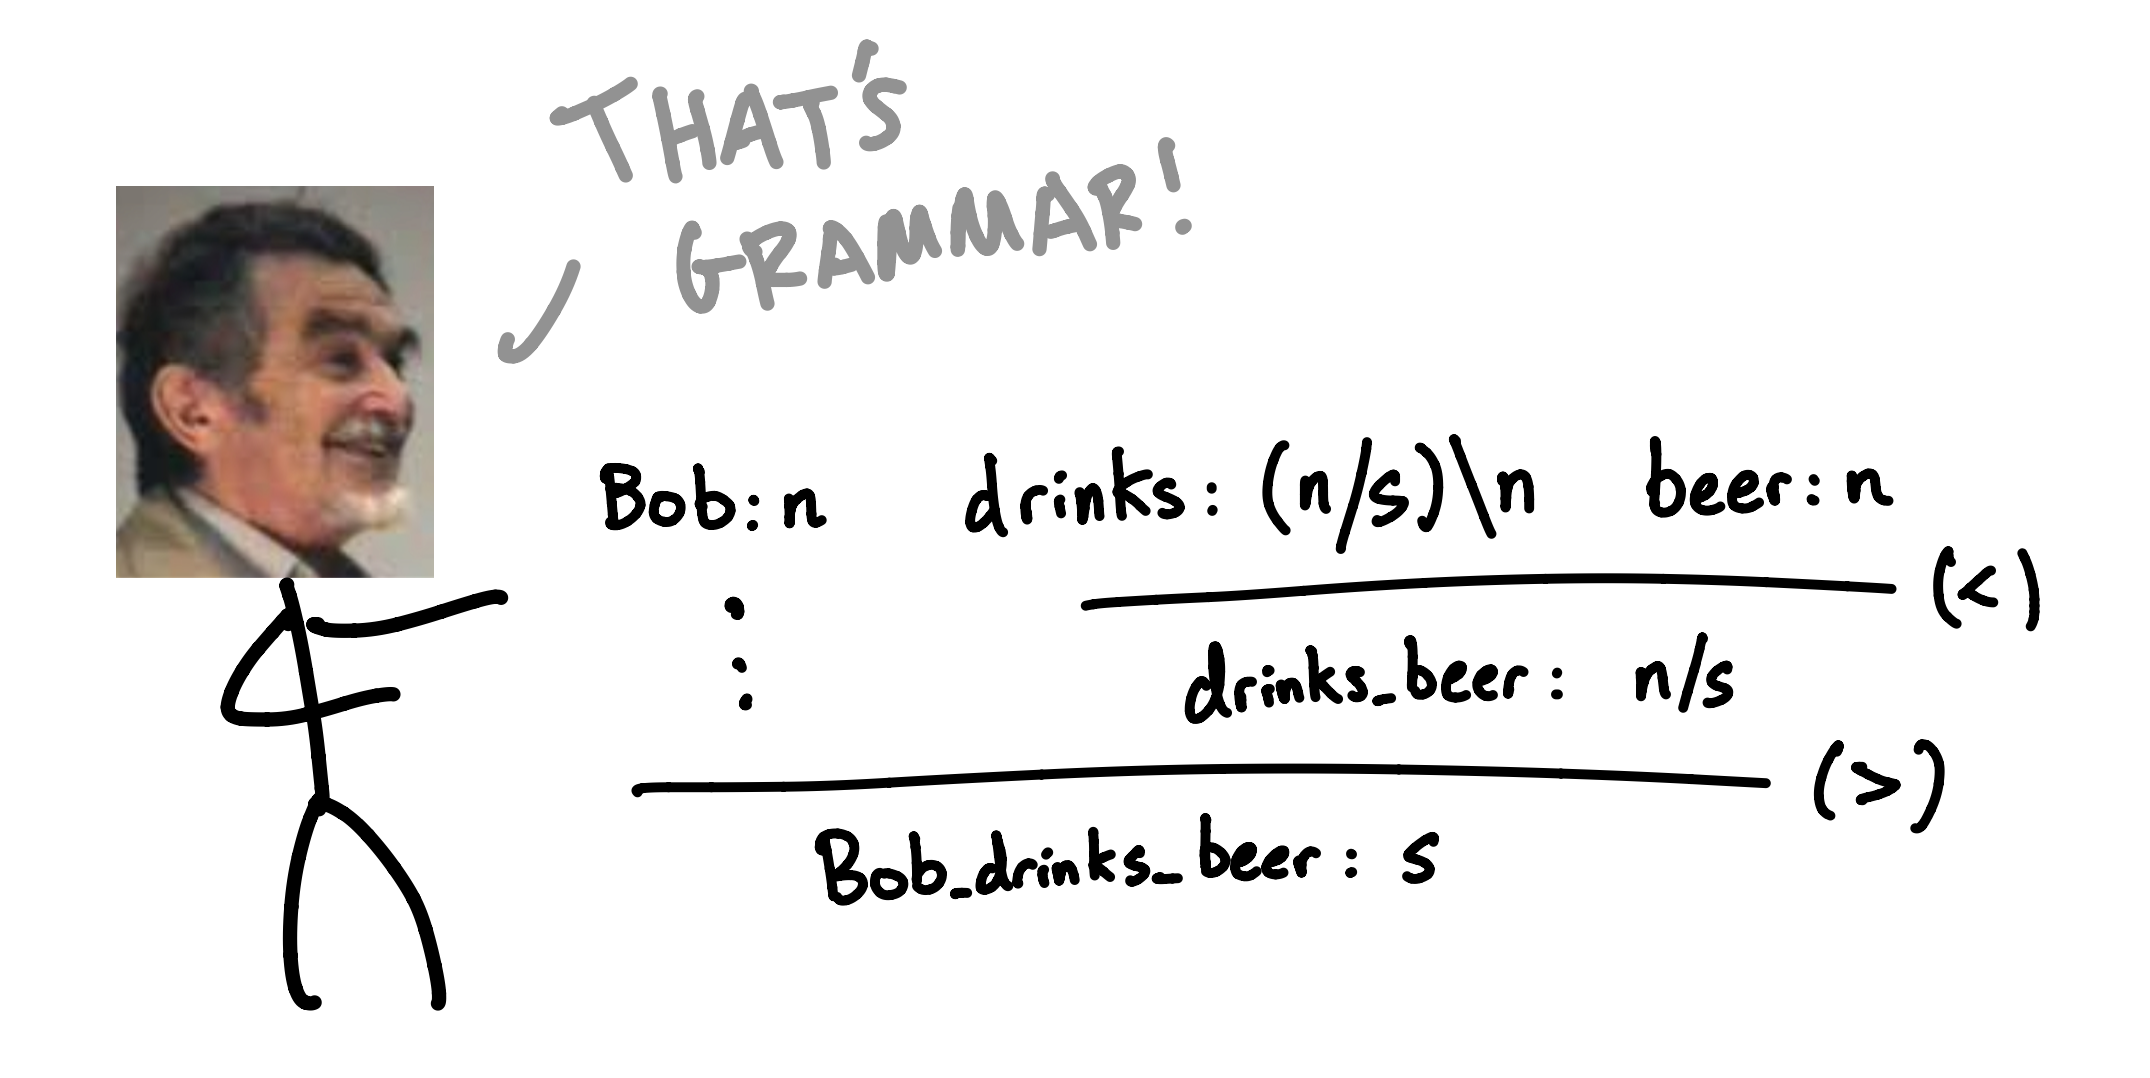
\includegraphics{figures/cartoons/lambek1}}
\caption{In English, we may consider a noun to have type $n$, and a transitive verb $(n/s)\setminus n$, to yield a well-formedness proof of \texttt{Bob drinks beer}. The type formation rules for such a grammar are intuitive. Apart from a stock of basic types $\mathbb{B}$ that contains special final types to indicate sentences, we have two type formation operators $(-/=)$ and $(- \setminus =)$, which along with their elimination rules establish a requirement that grammatical categories require other grammatical categories to their left or right. This is the essence of Lambek's calculi \textbf{NL} and \textbf{L}. CCGs keep the same minimal type-formations, but include extra sequent rules such as type-raising and cross-composition.}
\end{figure}

\begin{figure}[h!]
\centering
\scalebox{1}{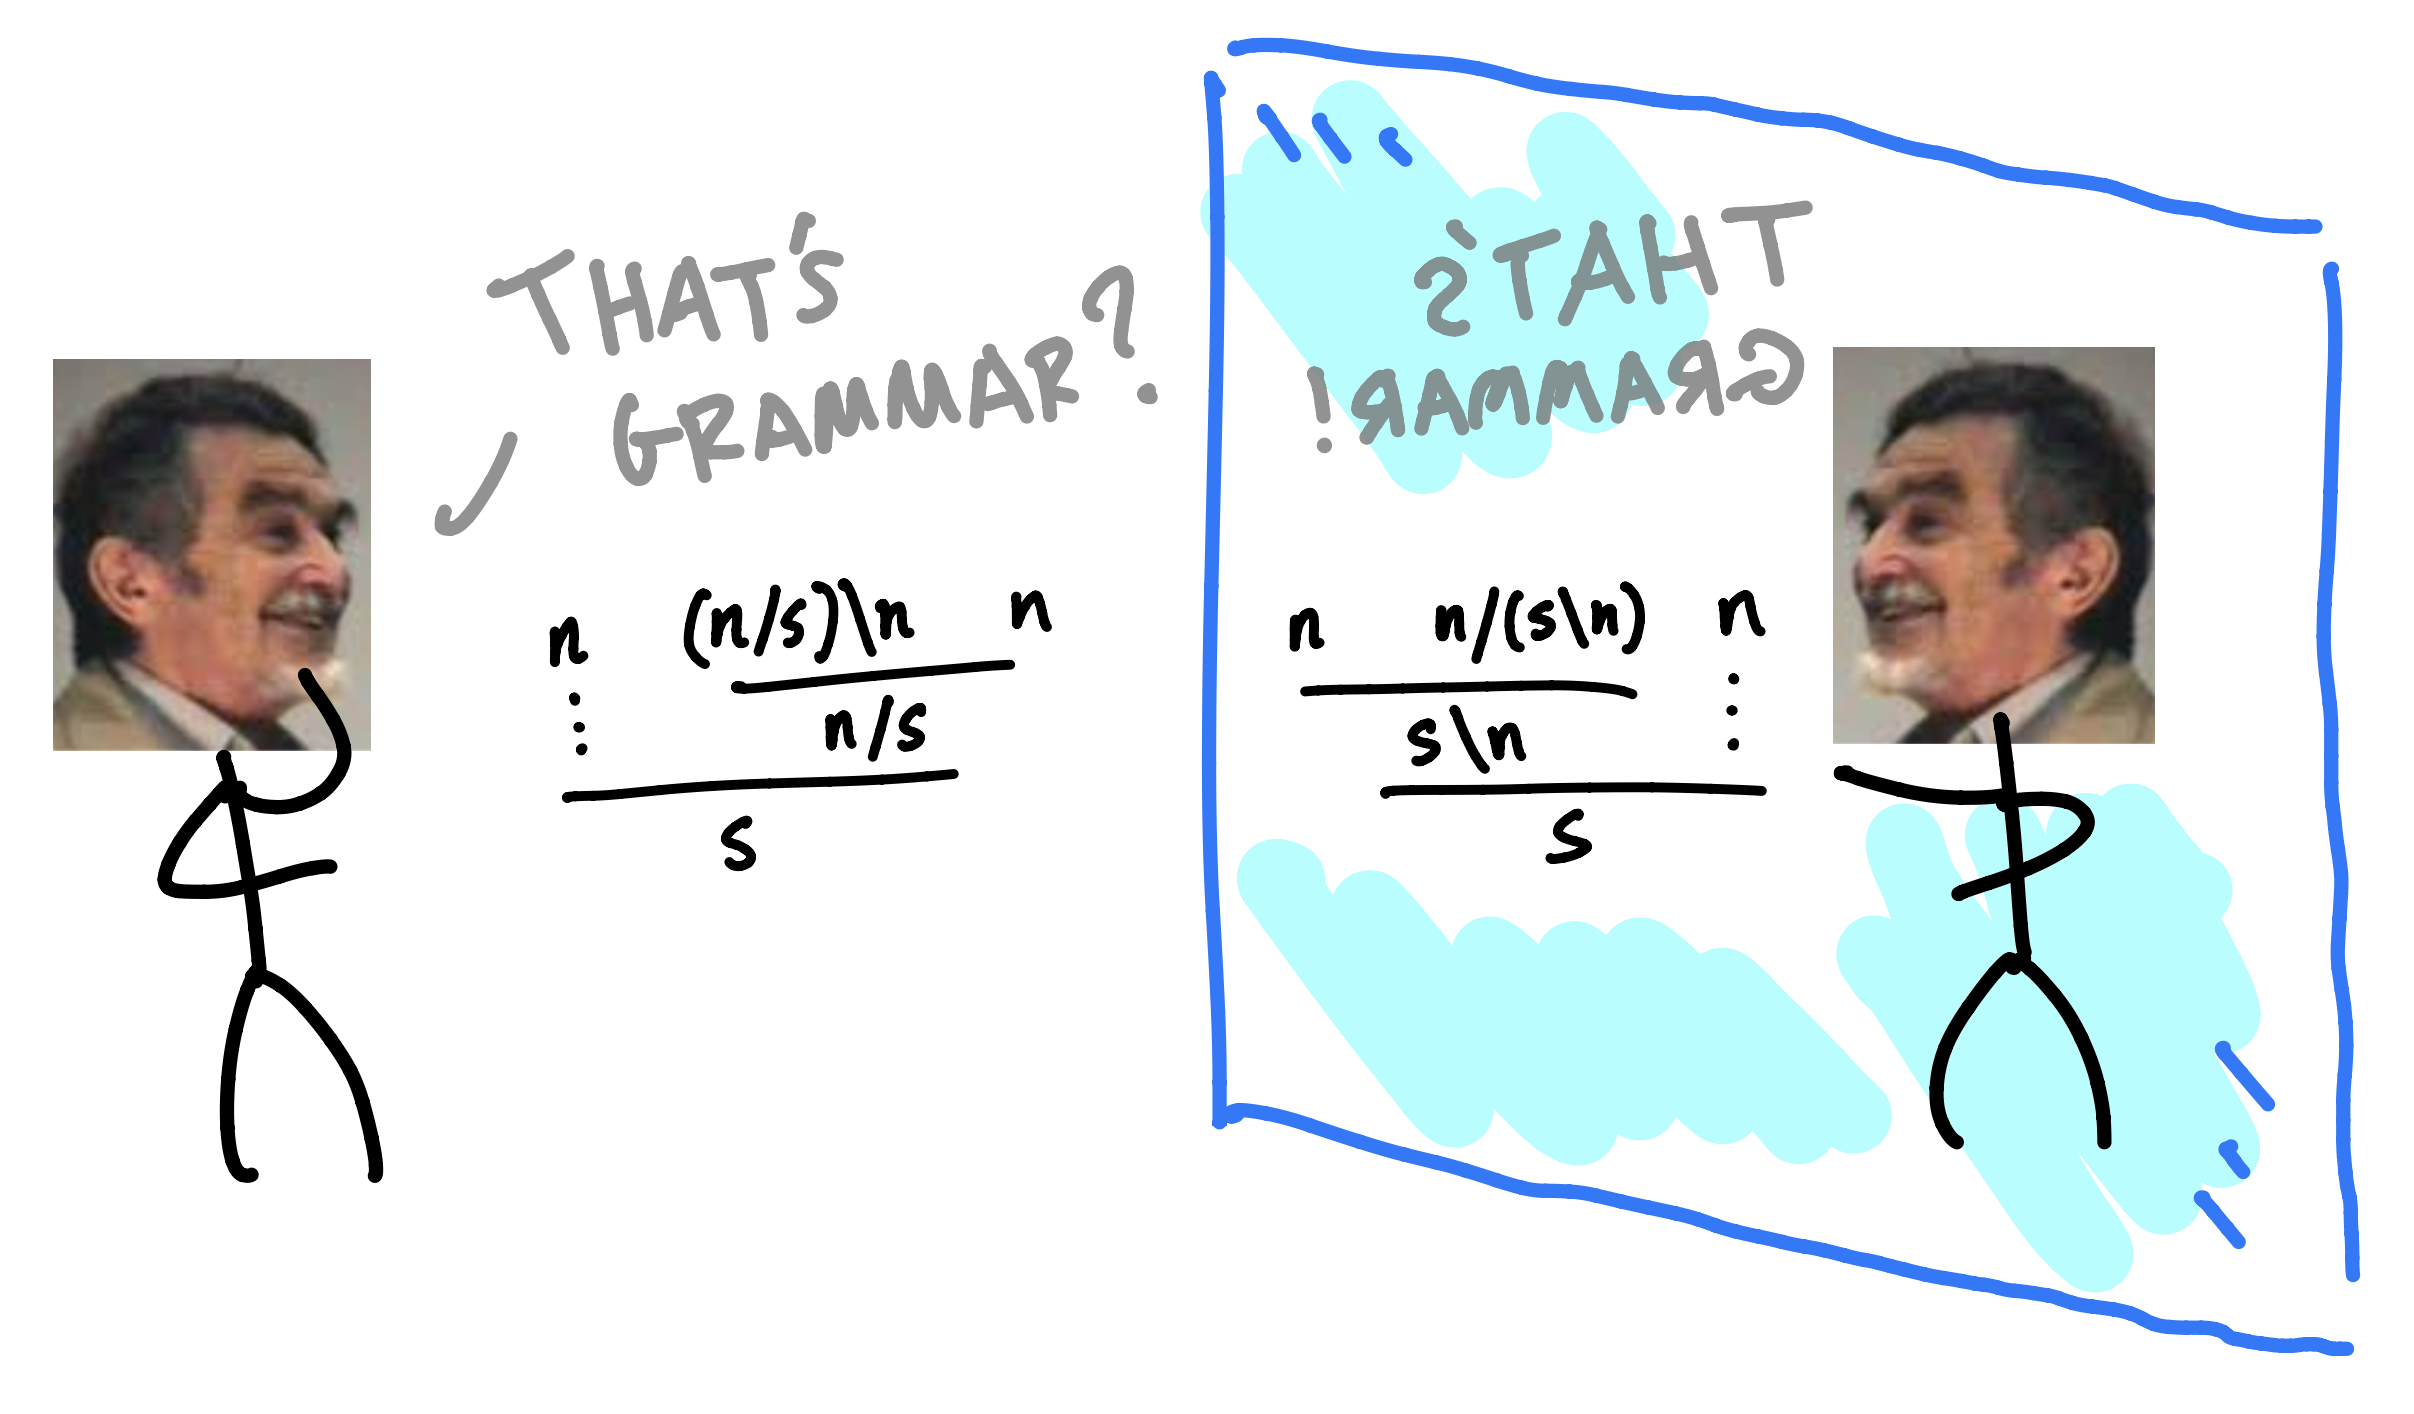
\includegraphics{figures/cartoons/lambek2}}
\caption{We can notice an asymmetry in the above formulation when we examine the transitive verb type $(n/s)\setminus n$ again; it asks first for a noun to the right, and then a noun to the left. We could just as well have asked for the nouns in the other order with the typing $(n/s)\setminus n$ and obtained all of the same proofs.}
\end{figure}

\begin{figure}[h!]
\centering
\scalebox{1}{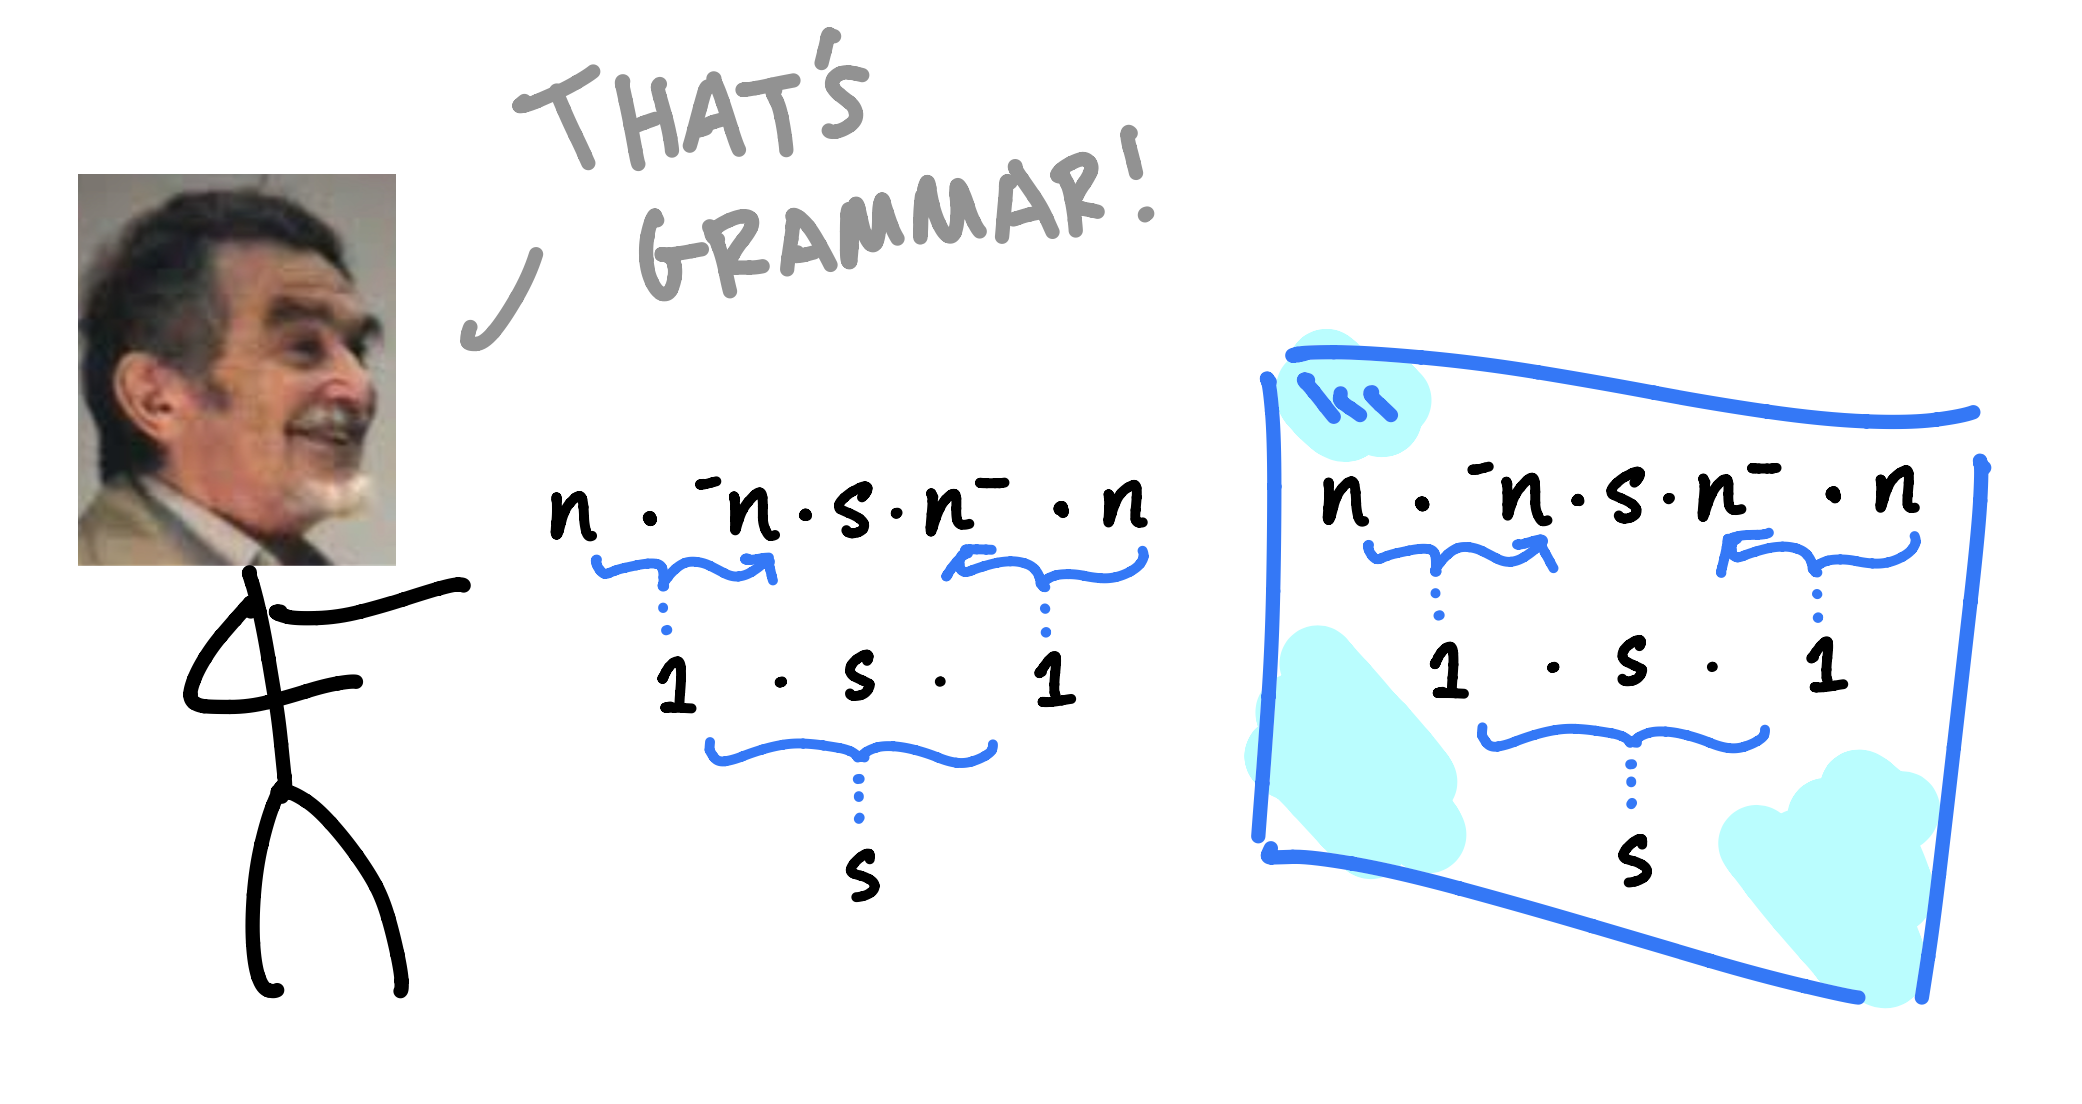
\includegraphics{figures/cartoons/lambek3}}
\caption{To eliminate this asymmetry, Lambek devised pregroup grammars. Whereas a group is a monoid with inverses up to left- and right-multiplication, a pregroup weakens the requirement for inverses so that all elements have distinct left- and right- inverses, denoted $x^{-1}$ and $^{-1}x$ respectively. Eliminating or introducing inverses is a non-identity relation on elements of the pregroup, so we have axioms of the form e.g. $x \cdot ^{-1}x \rightarrow 1 \rightarrow ^{1}x \cdot x$. In this formulation, denoting the multiplication with a dot, both $(n/s)\setminus n$ and $(n/s)\setminus n$ become $^{-1}n \cdot s \cdot n^{-1}$, which just wants a noun to the left and a noun to the right in whatever order to eliminate the flanking inverses to reveal the embedded sentence type. Now we can obtain the same proof of correctness as a series of algebraic reductions.

\begin{align*}
& &n \cdot (^{-1}n \cdot s \cdot n^{-1}) \cdot n\\
&\rightarrow &(n \cdot ^{-1}n) \cdot s \cdot (n^{-1} \cdot n)\\
&\rightarrow & 1 \cdot s \cdot 1\\
&\rightarrow & s
\end{align*}
}
\end{figure}
\clearpage

\subsection{Coecke's Composition}

\begin{figure}[h!]
\centering
\scalebox{0.9}{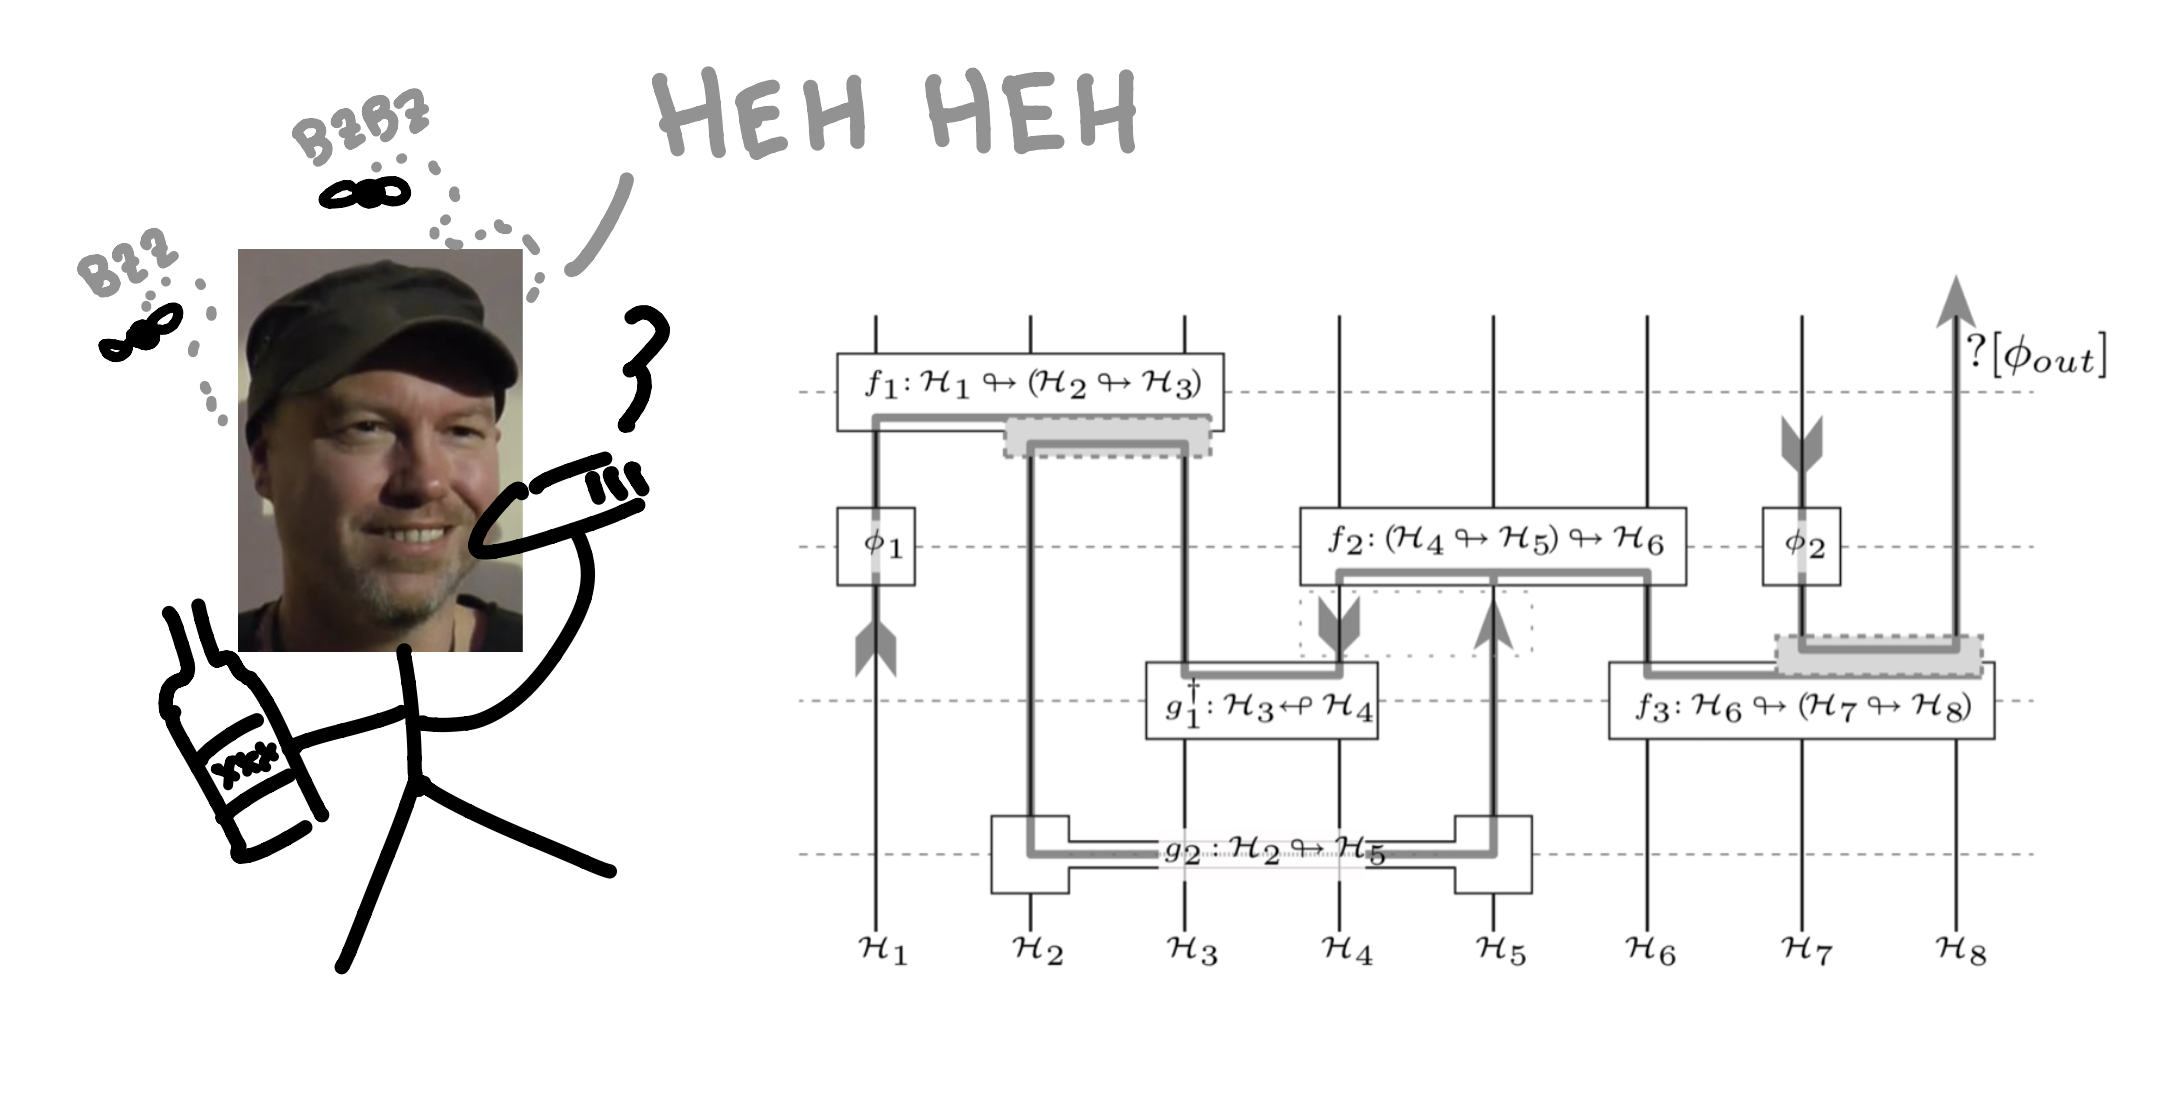
\includegraphics{figures/cartoons/bob1}}
\caption{Meanwhile, an underground grunge vagabond moonlighting as a quantum physicist moonlighting as a computer scientist was causing a shortage of cigars and whiskey in a small English town. He noticed a funny thing about the composition of multiple non-destructive measurements of a quantum system, which was that information could be carried, or flow, between them. So he wrote a paper \bR invitationtoquantum \e, which contained informal diagrams that looked like this.}
\end{figure}

\begin{figure}[h!]
\centering
\scalebox{0.9}{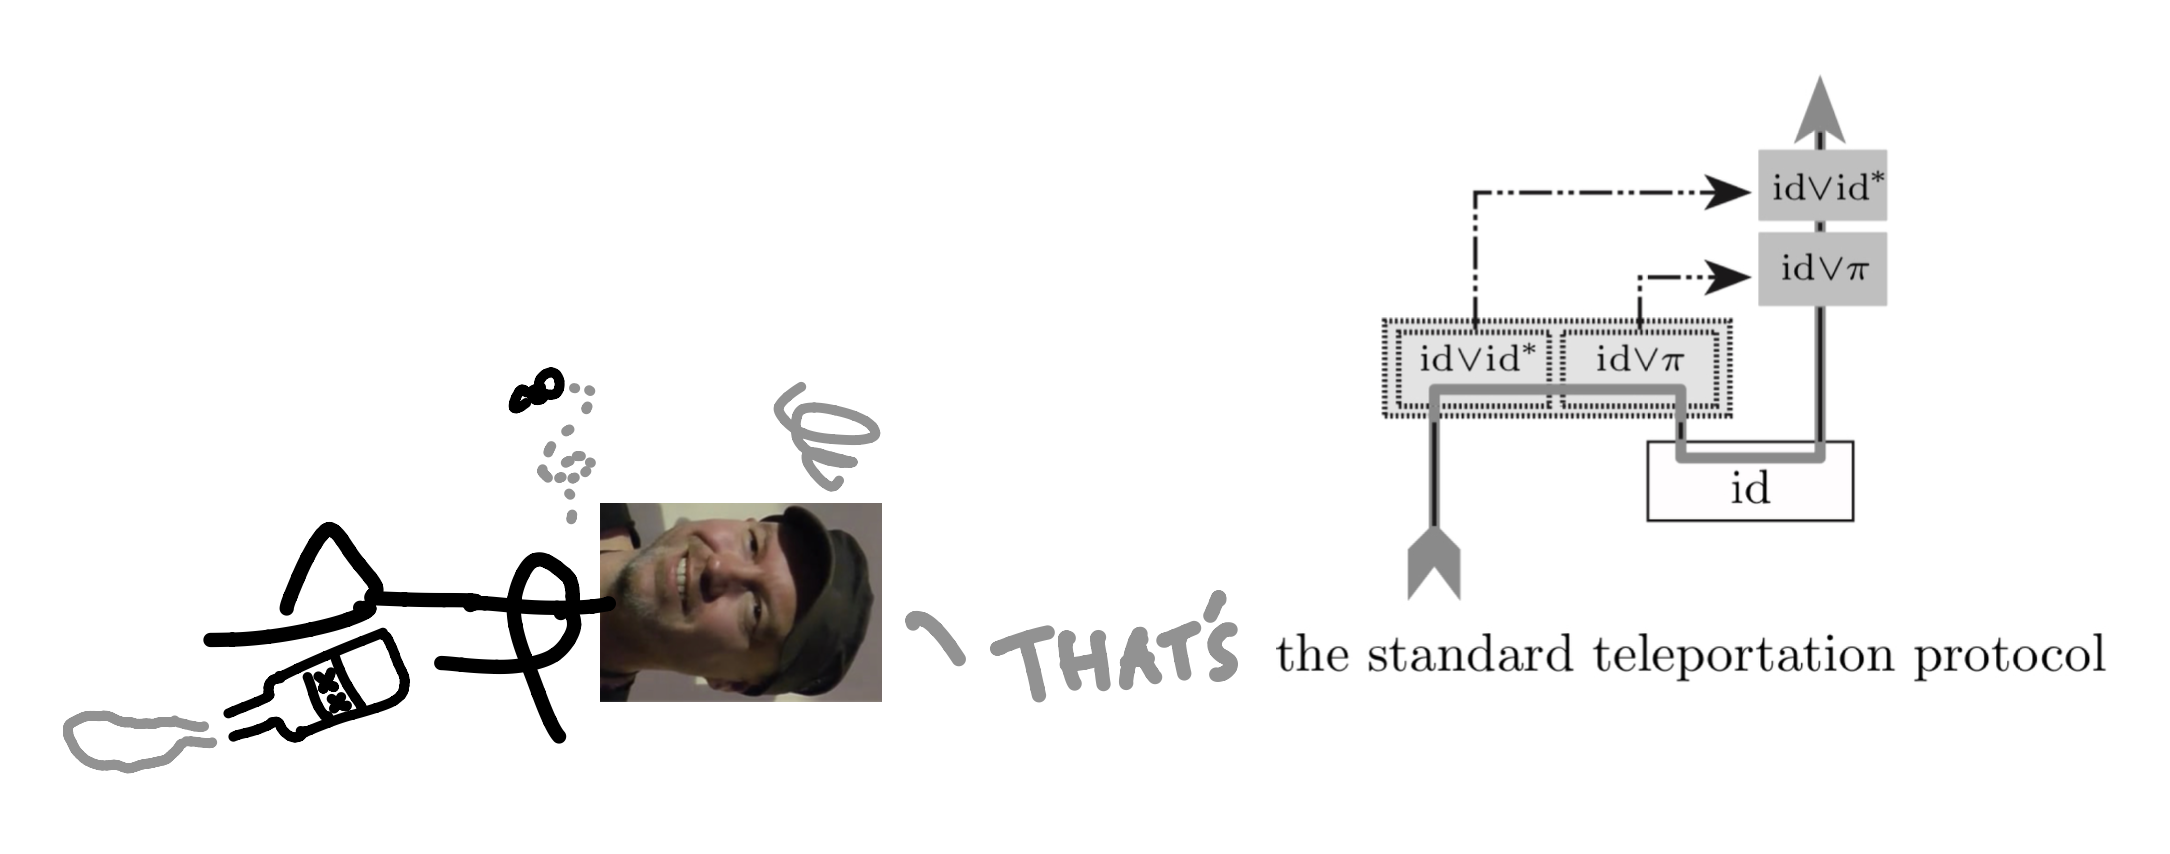
\includegraphics{figures/cartoons/bob2}}
\caption{There were two impressive things about these diagrams. First, the effects such as transparencies for text boxes and curved serifs for angled arrows give a modern feel, but they were done manually in macdraw, the diagrammatic equivalent of sticks and stones. Second, though the diagrams were informal, they provided a way to visualise and reason about entanglement that was impossible by staring at the equivalent matrix formulation of the same composite operator. The most important diagram for our story was this one, which captures the information flow of quantum teleportation.}
\end{figure}
\clearpage

\subsection{Categorical quantum mechanics}

\begin{figure}[h!]
\centering
\scalebox{1}{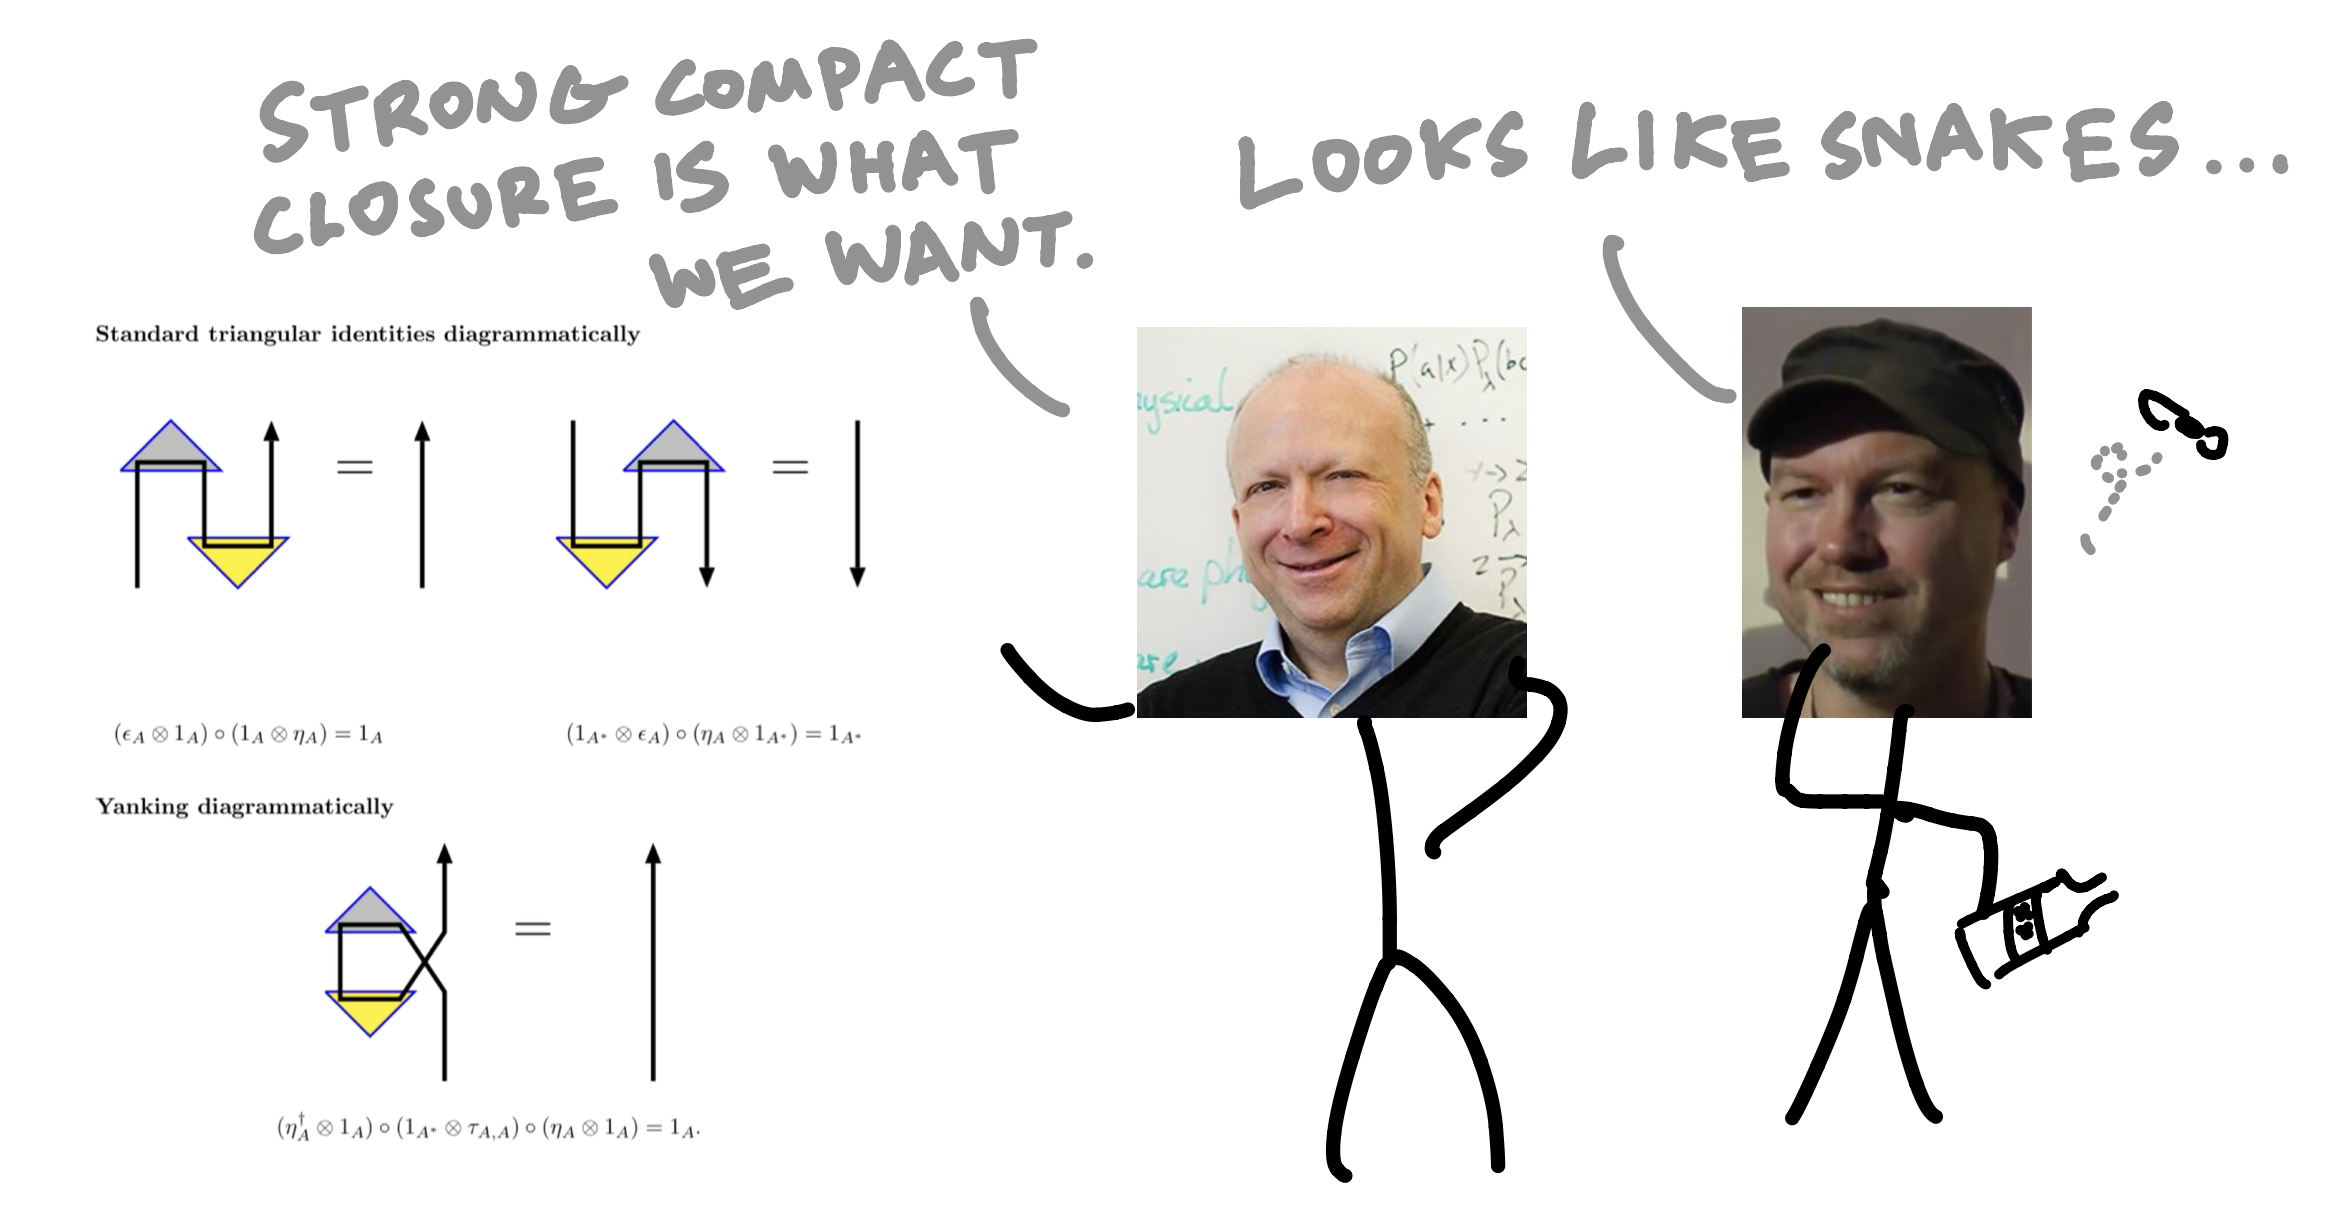
\includegraphics{figures/cartoons/samson}}
\caption{Category theorists and physicists such as Abramsky and Baez were excited about these diagrams, which looked like string diagrams waiting to be made formal. The graphical cups and caps in the important diagram were determined to correspond to a special form of symmetric monoidal closed category called strong compact closed.}
\end{figure}

\begin{figure}[h!]
\centering
\scalebox{1}{
\includegraphics{figures/cartoons/cjiso}}
\caption{Diagrammatically, reasoning in a strongly compact closed category amounts to ignoring the usual requirement of processiveness and forgetting the distinction between inputs and outputs, so that "future" outputs could curl back and be "past" inputs. This formulation also gave insight into the structure of quantum mechanics. For example, the process-state duality of strong compact closure manifested as the Choi–Jamiołkowski isomorphism.}
\end{figure}

\begin{figure}[h!]
\centering
\scalebox{1}{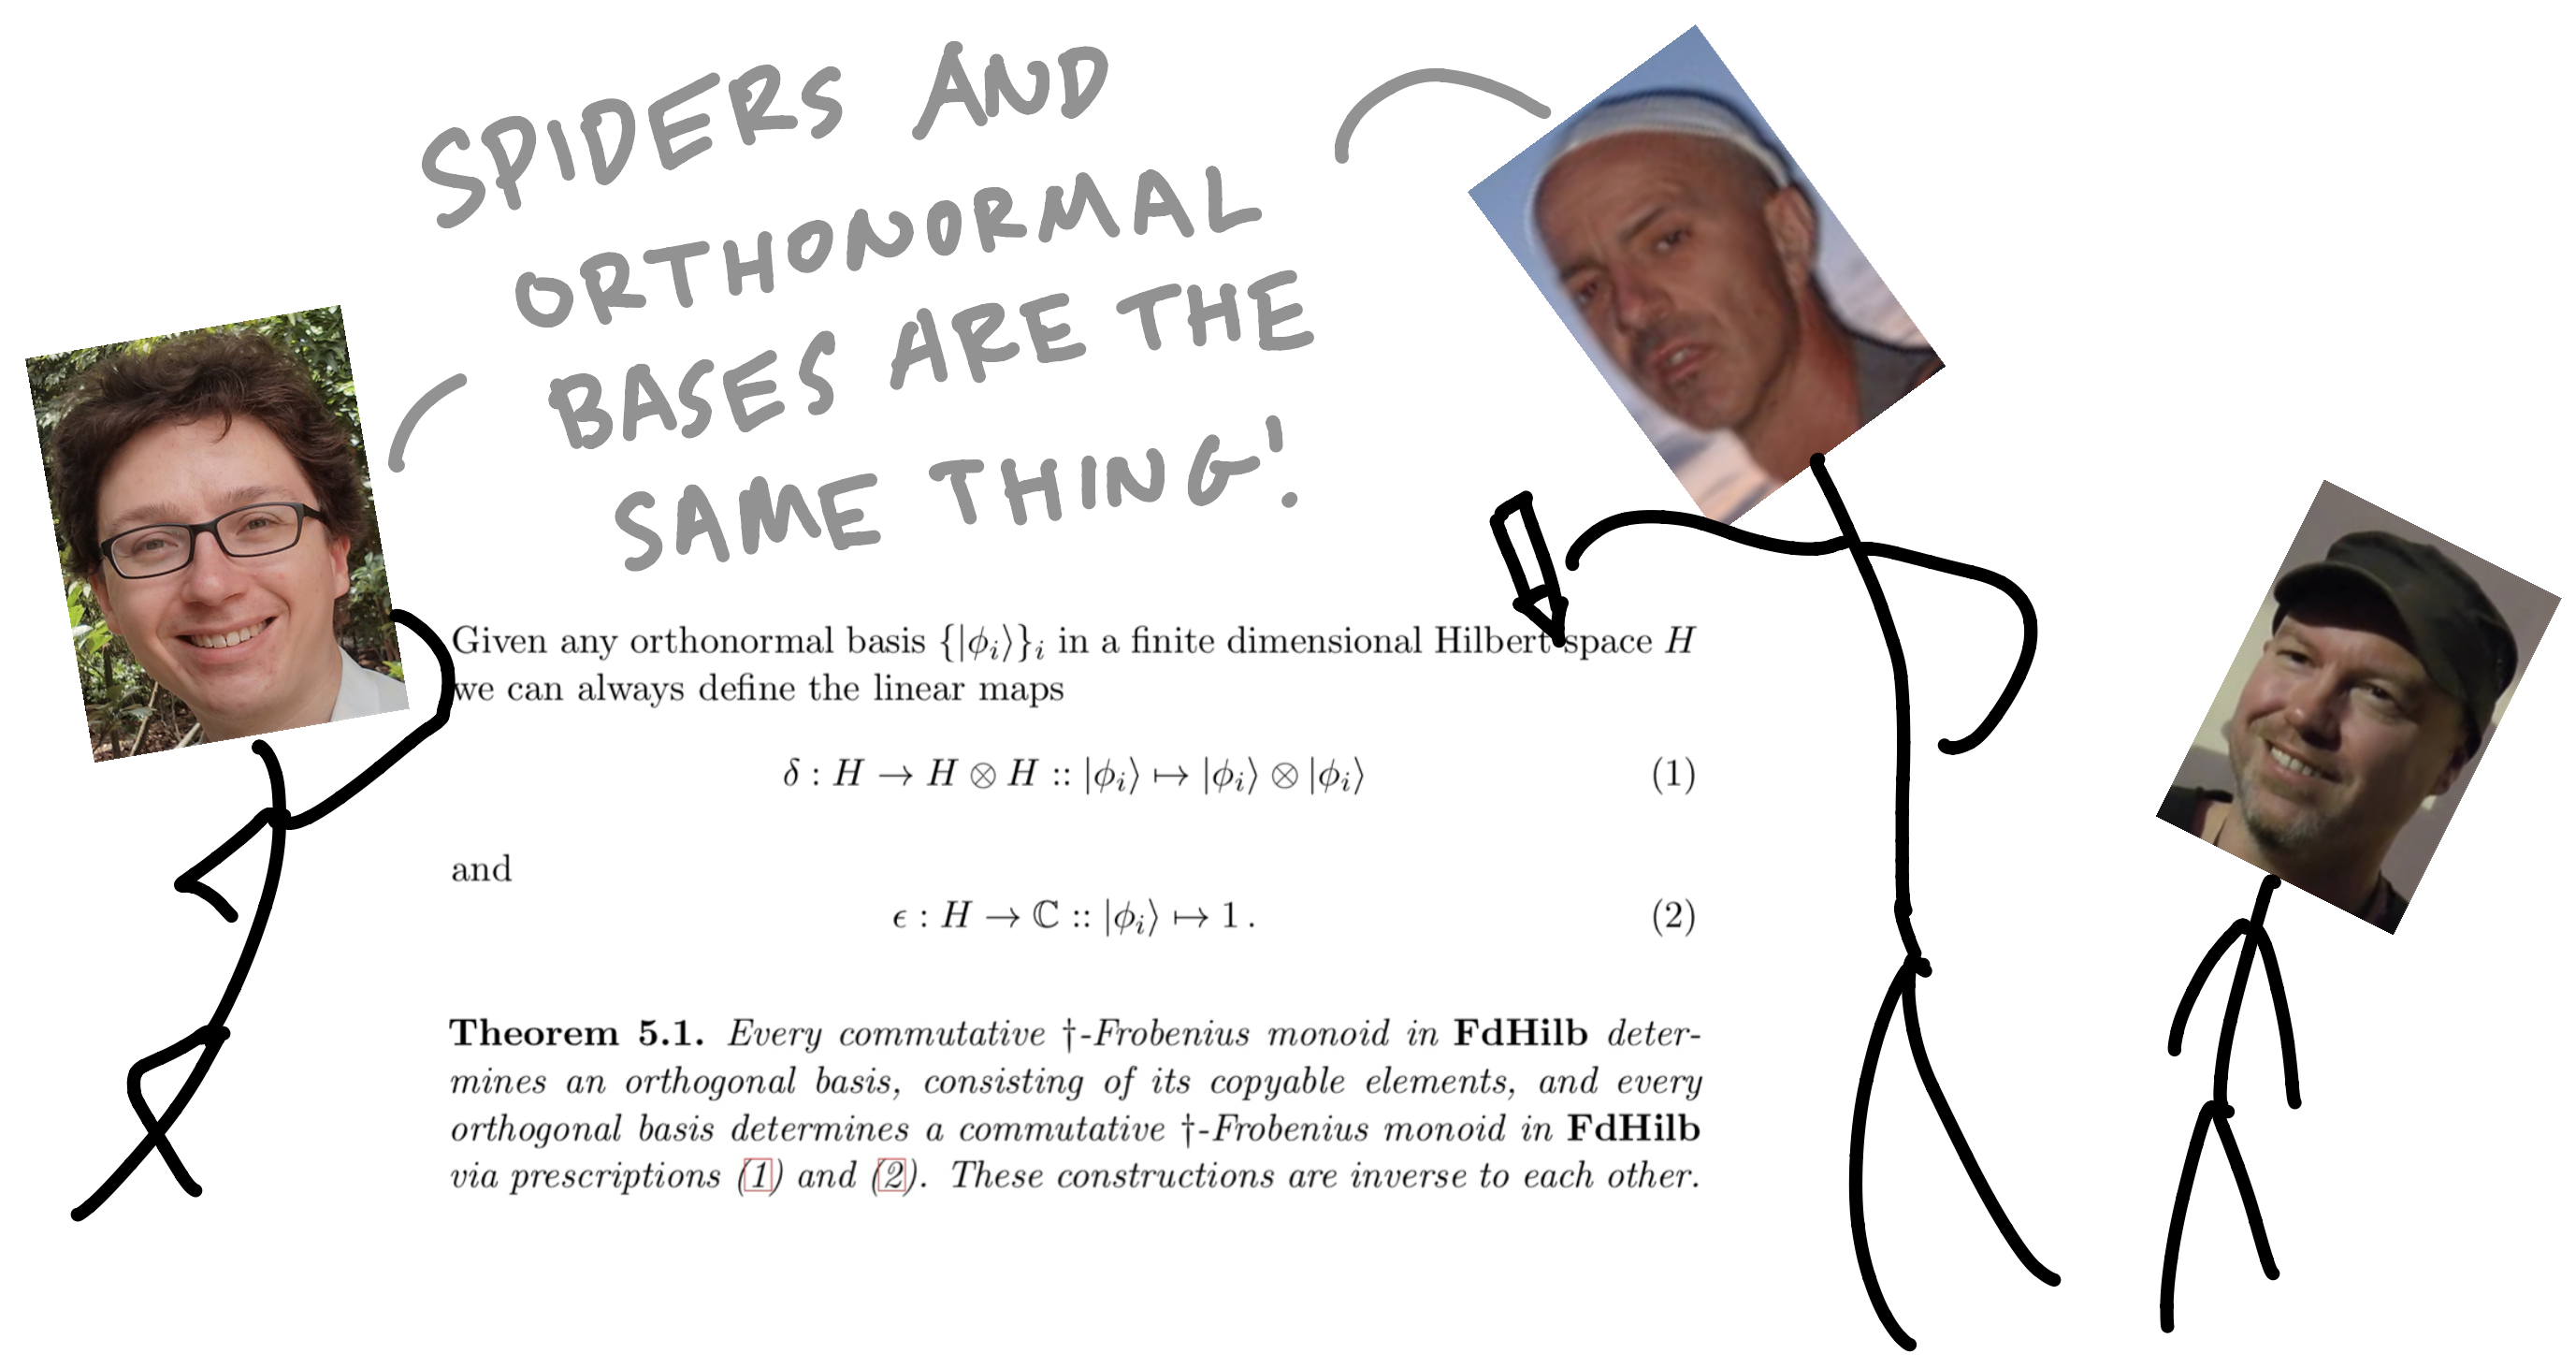
\includegraphics{figures/cartoons/spiders}}
\caption{However, dealing with superpositions necessitated using summation operators within diagrams, which is cumbersome to write especially when dealing with even theoretically simple Bell states. An elegant diagrammatic simplification arose with the observation that special-$\dagger$-frobenius algebras \bR classicquantumstruct \e, or spiders, correspond to choices of orthonormal bases \bR novelchar \e in \textbf{FdHilb}, the ambient setting of finite-dimensional hilbert spaces. Not only did this remove the need for summation operators, it also revealed that strong compact closure was a derived, rather than fundamental structure, since spiders induce compact closed structure.}
\end{figure}

\begin{figure}[h!]
\centering
\scalebox{1}{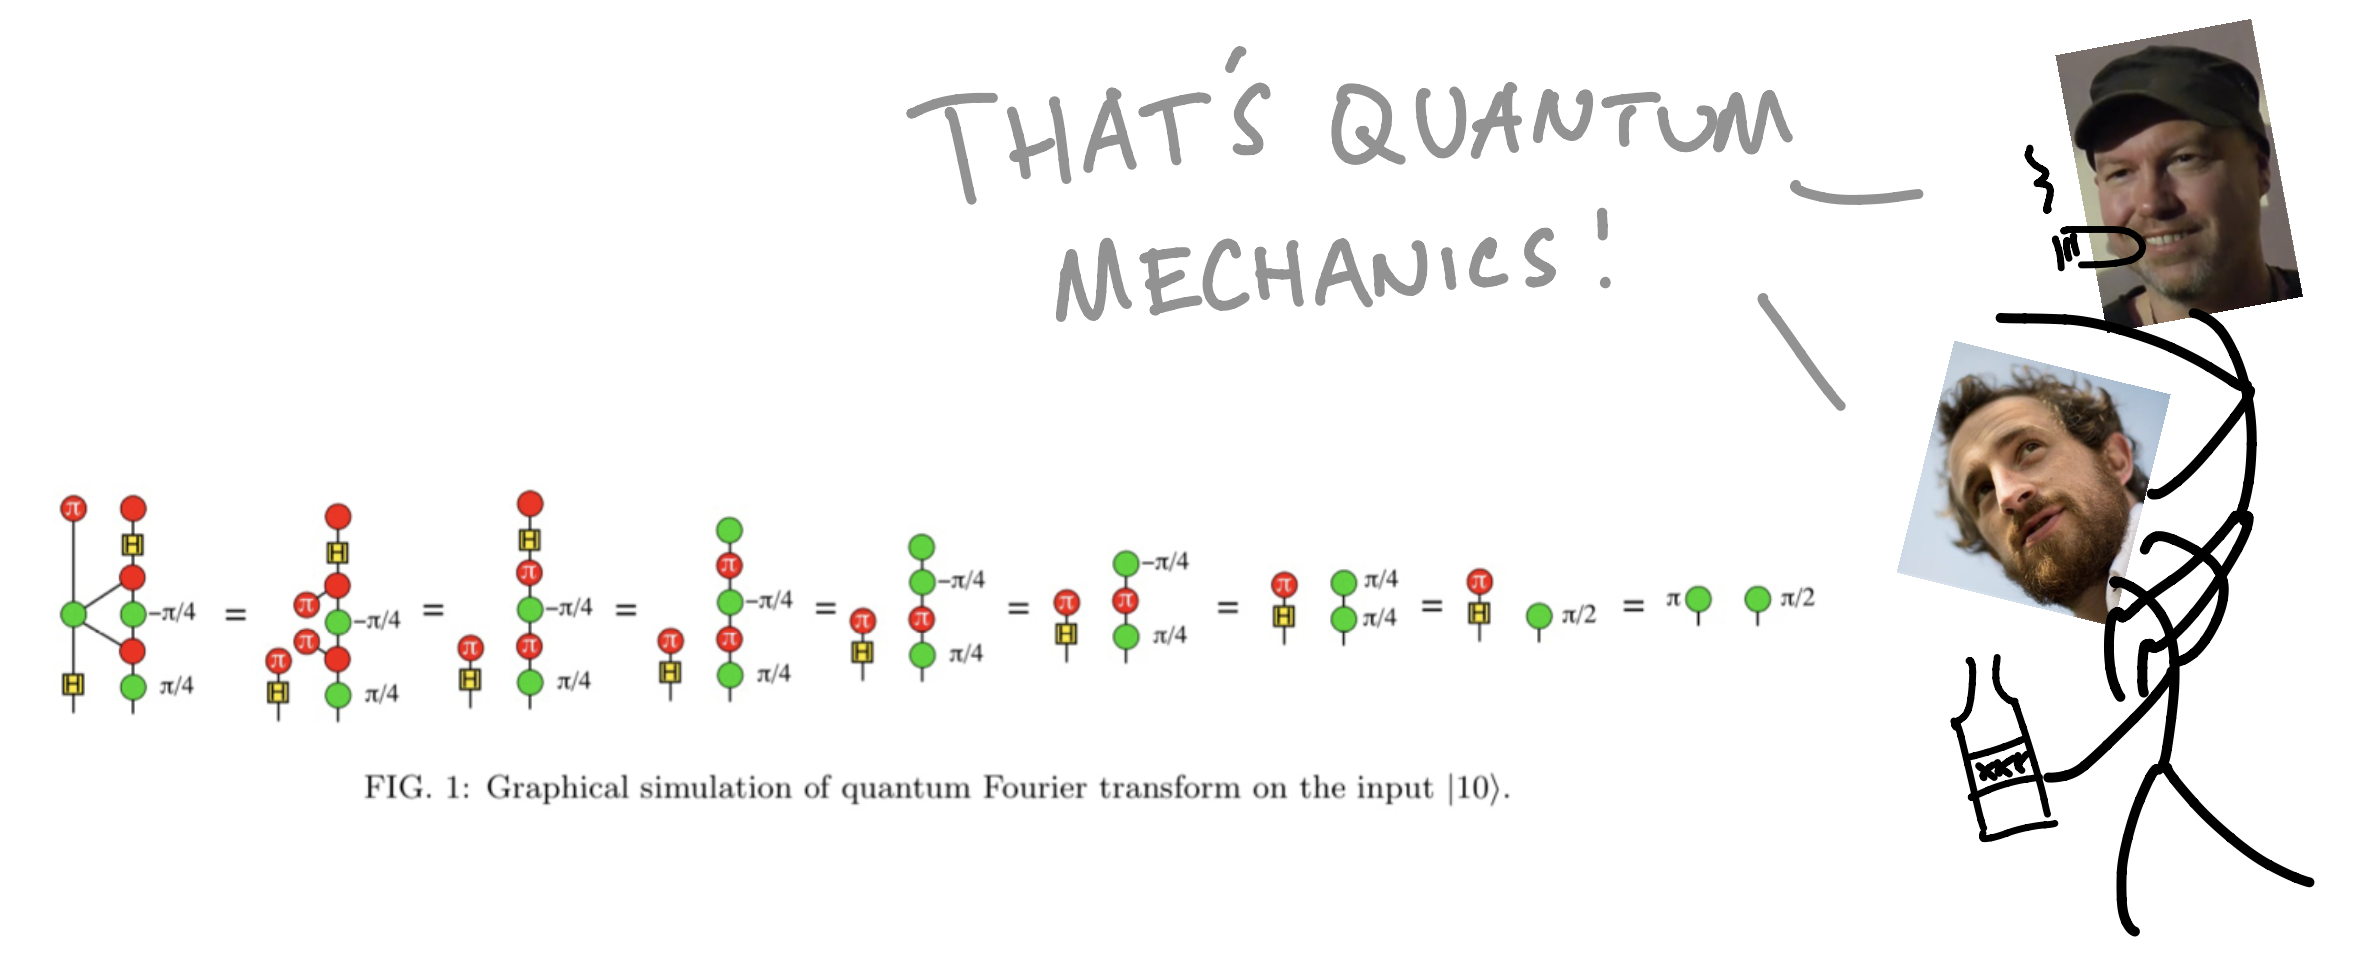
\includegraphics{figures/cartoons/ross}}
\caption{And so the stage was set for a purely diagrammatic treatment of ZX quantum mechanics. The story of ZX diverges away from our interest, so I will summarise what happened afterwards. In no particular order, the development of ZX went on to accommodate a third axis of measurement to yield a ZXW calculus \bR CITE \e, the systems were proven to be complete \bR CITES \e, there are at the time of writing two expository books \bR CITES \e, and ZX-variants are becoming an industry standard for quantum circuit specification and rewriting \bR CITE \e.}
\end{figure}
\clearpage

\subsection{Enter computational linguistics}

\begin{figure}[h!]
\centering
\scalebox{1}{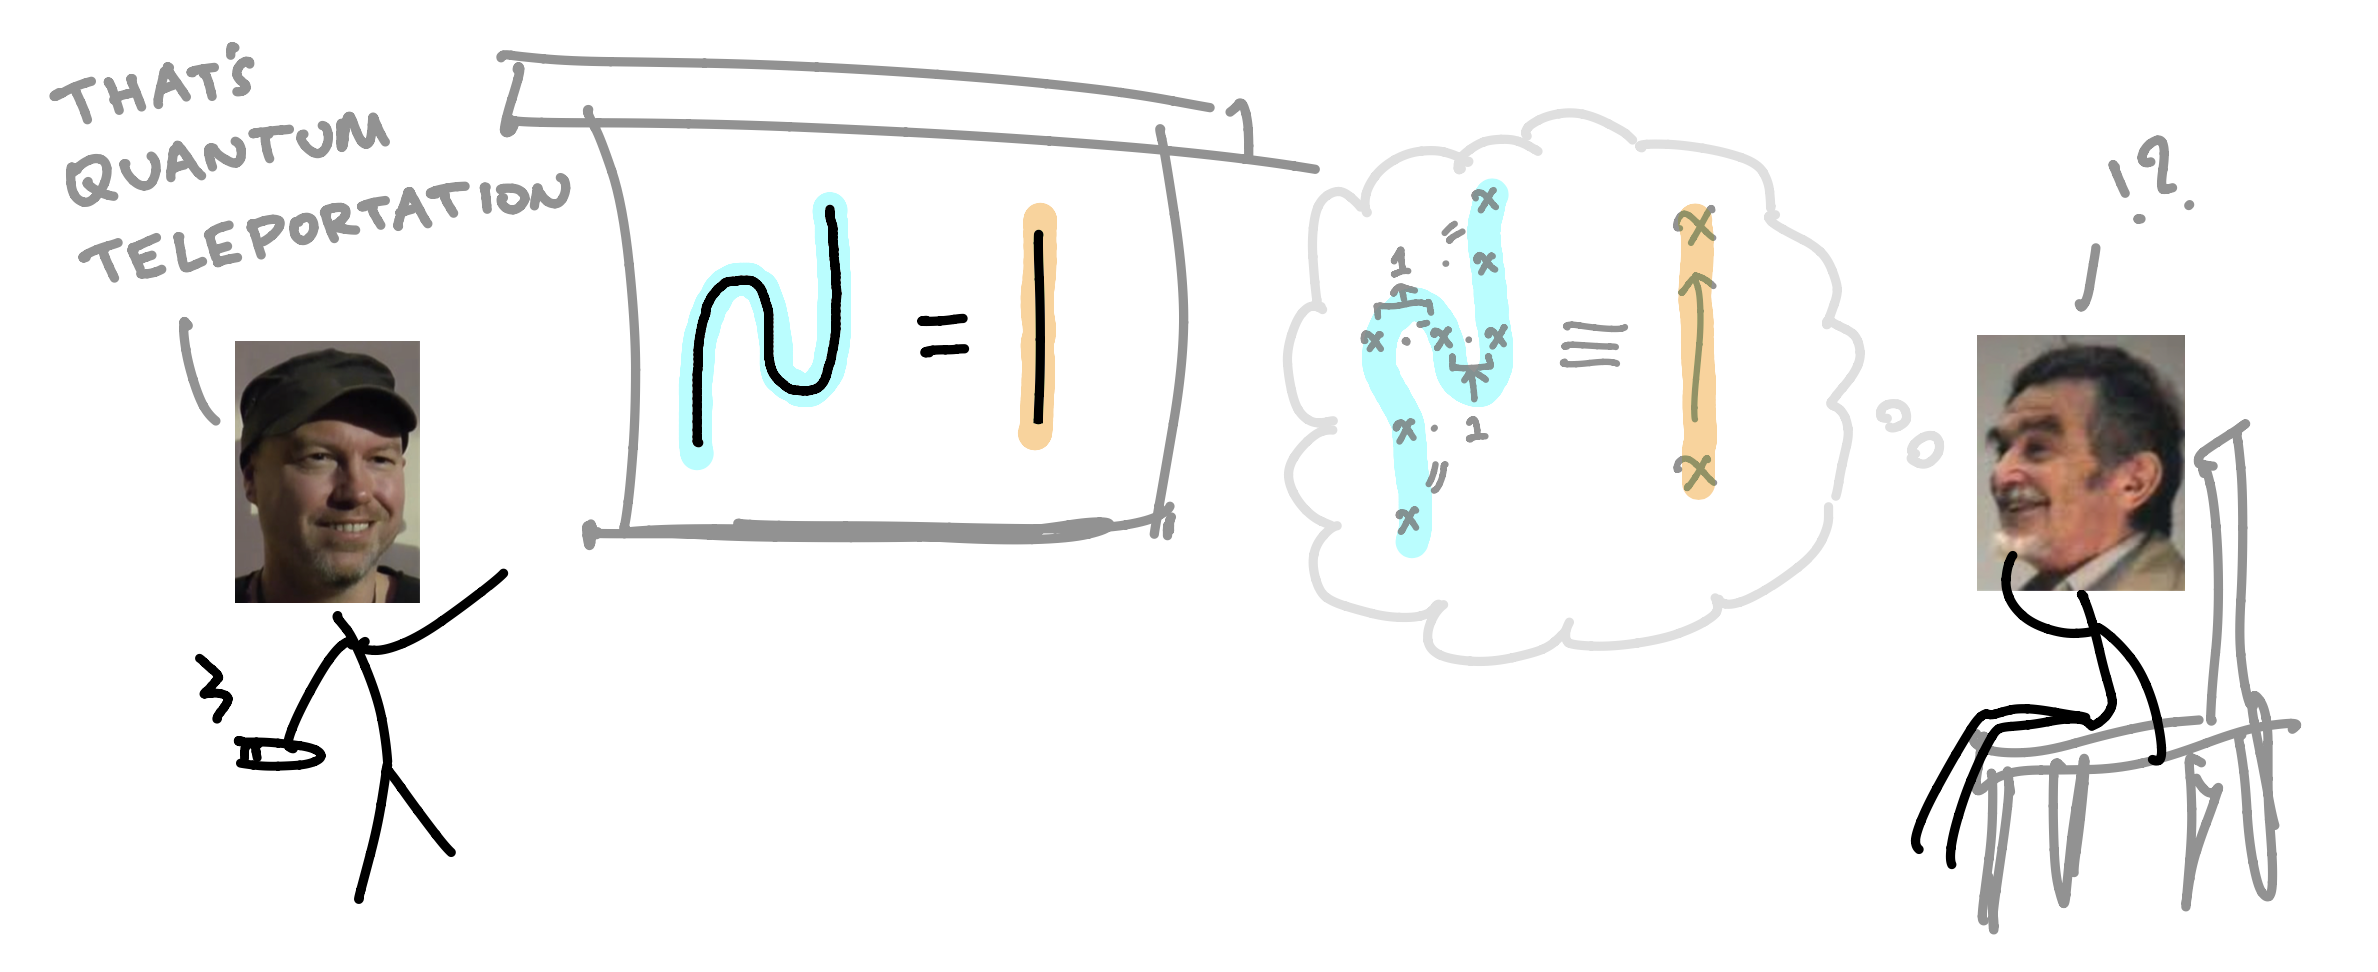
\includegraphics{figures/cartoons/boblambek1}}
\caption{Somewhere in Canada at the turn of the millenium, Bob met Jim, who saw something familiar about the diagram for quantum teleportation. The snake equation for compact closure looked a lot like the categorified version of introducing and eliminating pregroup types.
}
\end{figure}

\begin{figure}[h!]
\centering
\scalebox{1}{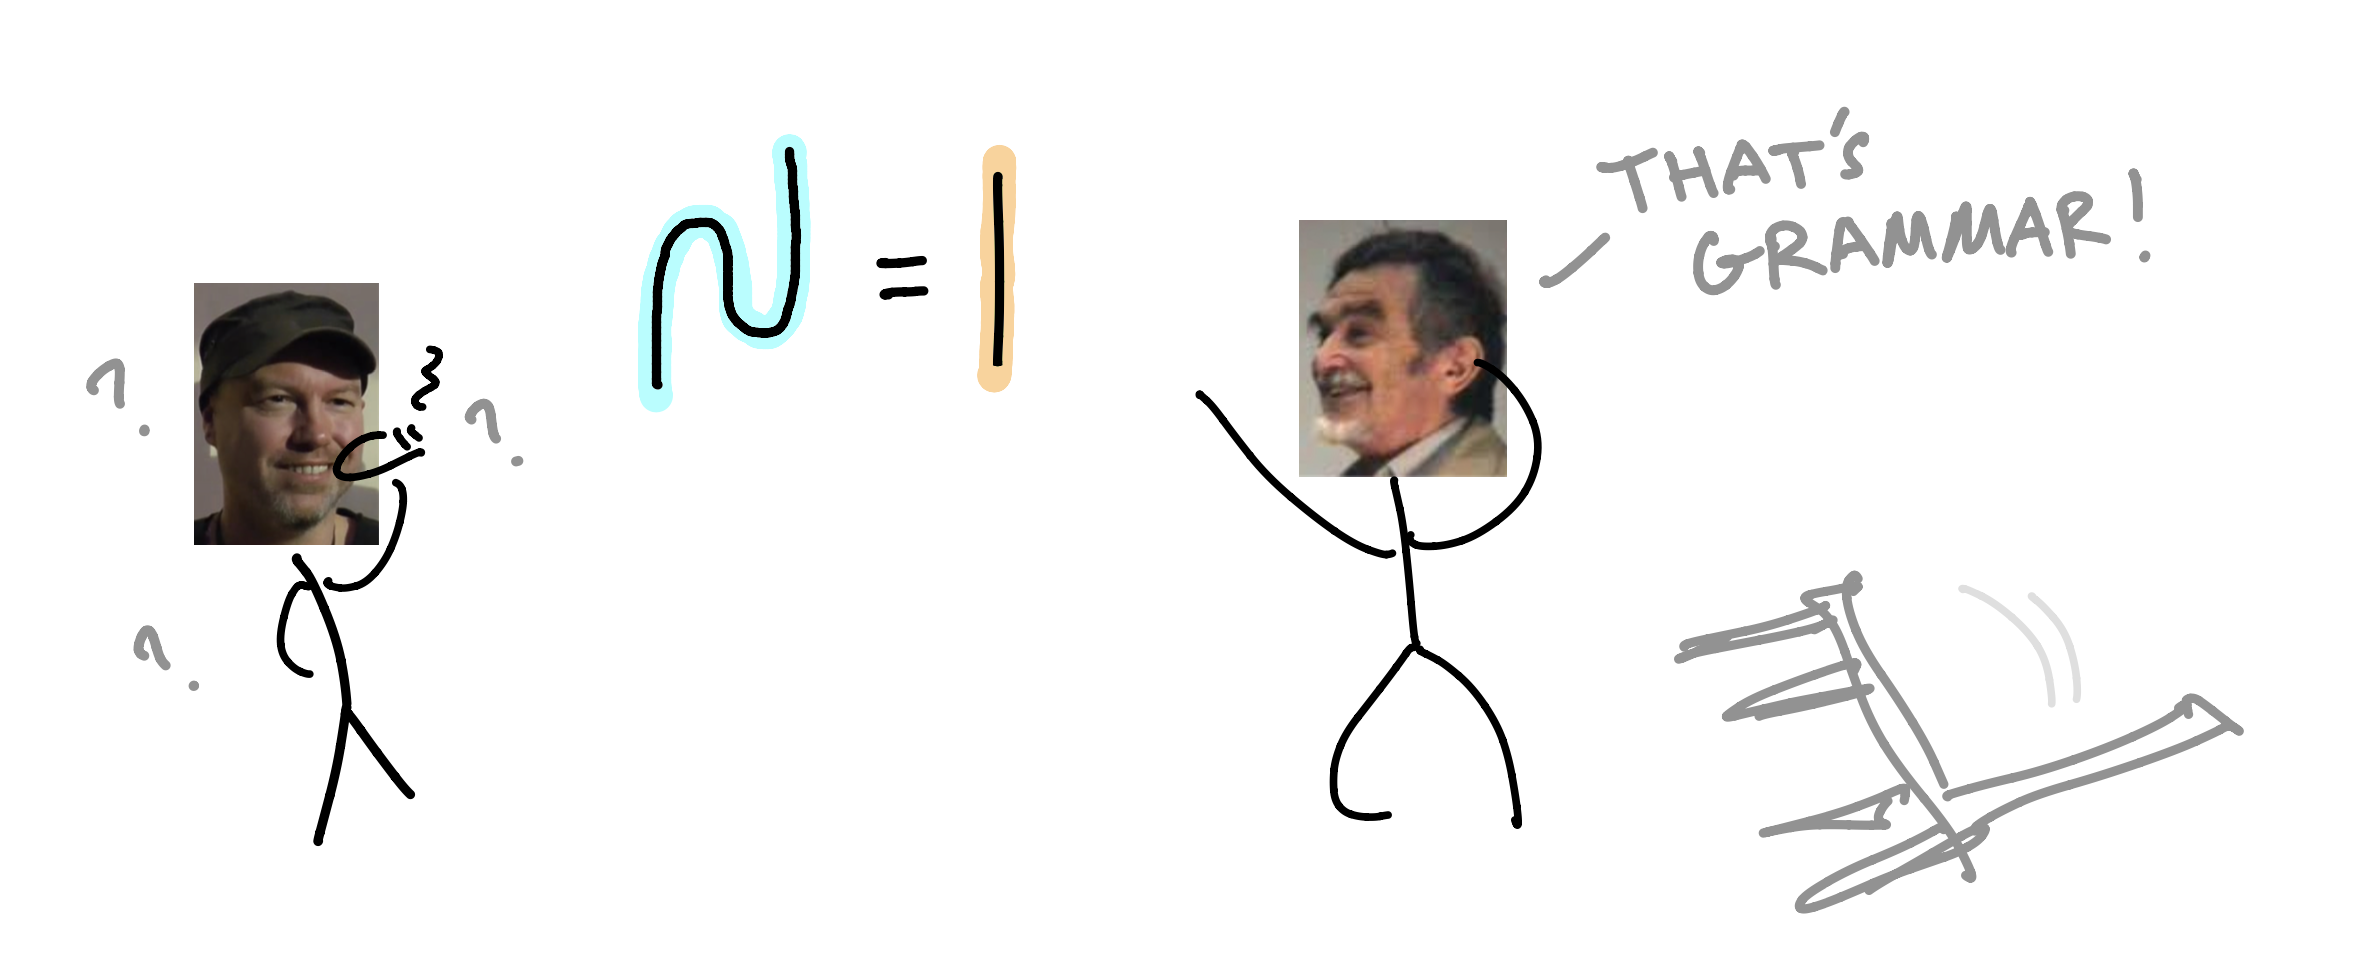
\includegraphics{figures/cartoons/boblambek2}}
\caption{Bob and Jim's meeting put the adjectives \emph{compositional} and \emph{categorical} on the same table, but the cake wasn't ready. Two more actors Steve and Mehrnoosh were required to introduce \emph{distributional}, which refers to Firth's maxim \bR CITE \e "you shall know a word by the company it keeps". In its modern incarnation, this refers generally to vector-based semantics for words, where it is desirable but not necessarily so (as in the case of generic latent space embeddings by an autoencoder) that proximity of vectors models semantic closeness.}
\end{figure}

\begin{figure}[h!]
\centering
\scalebox{1}{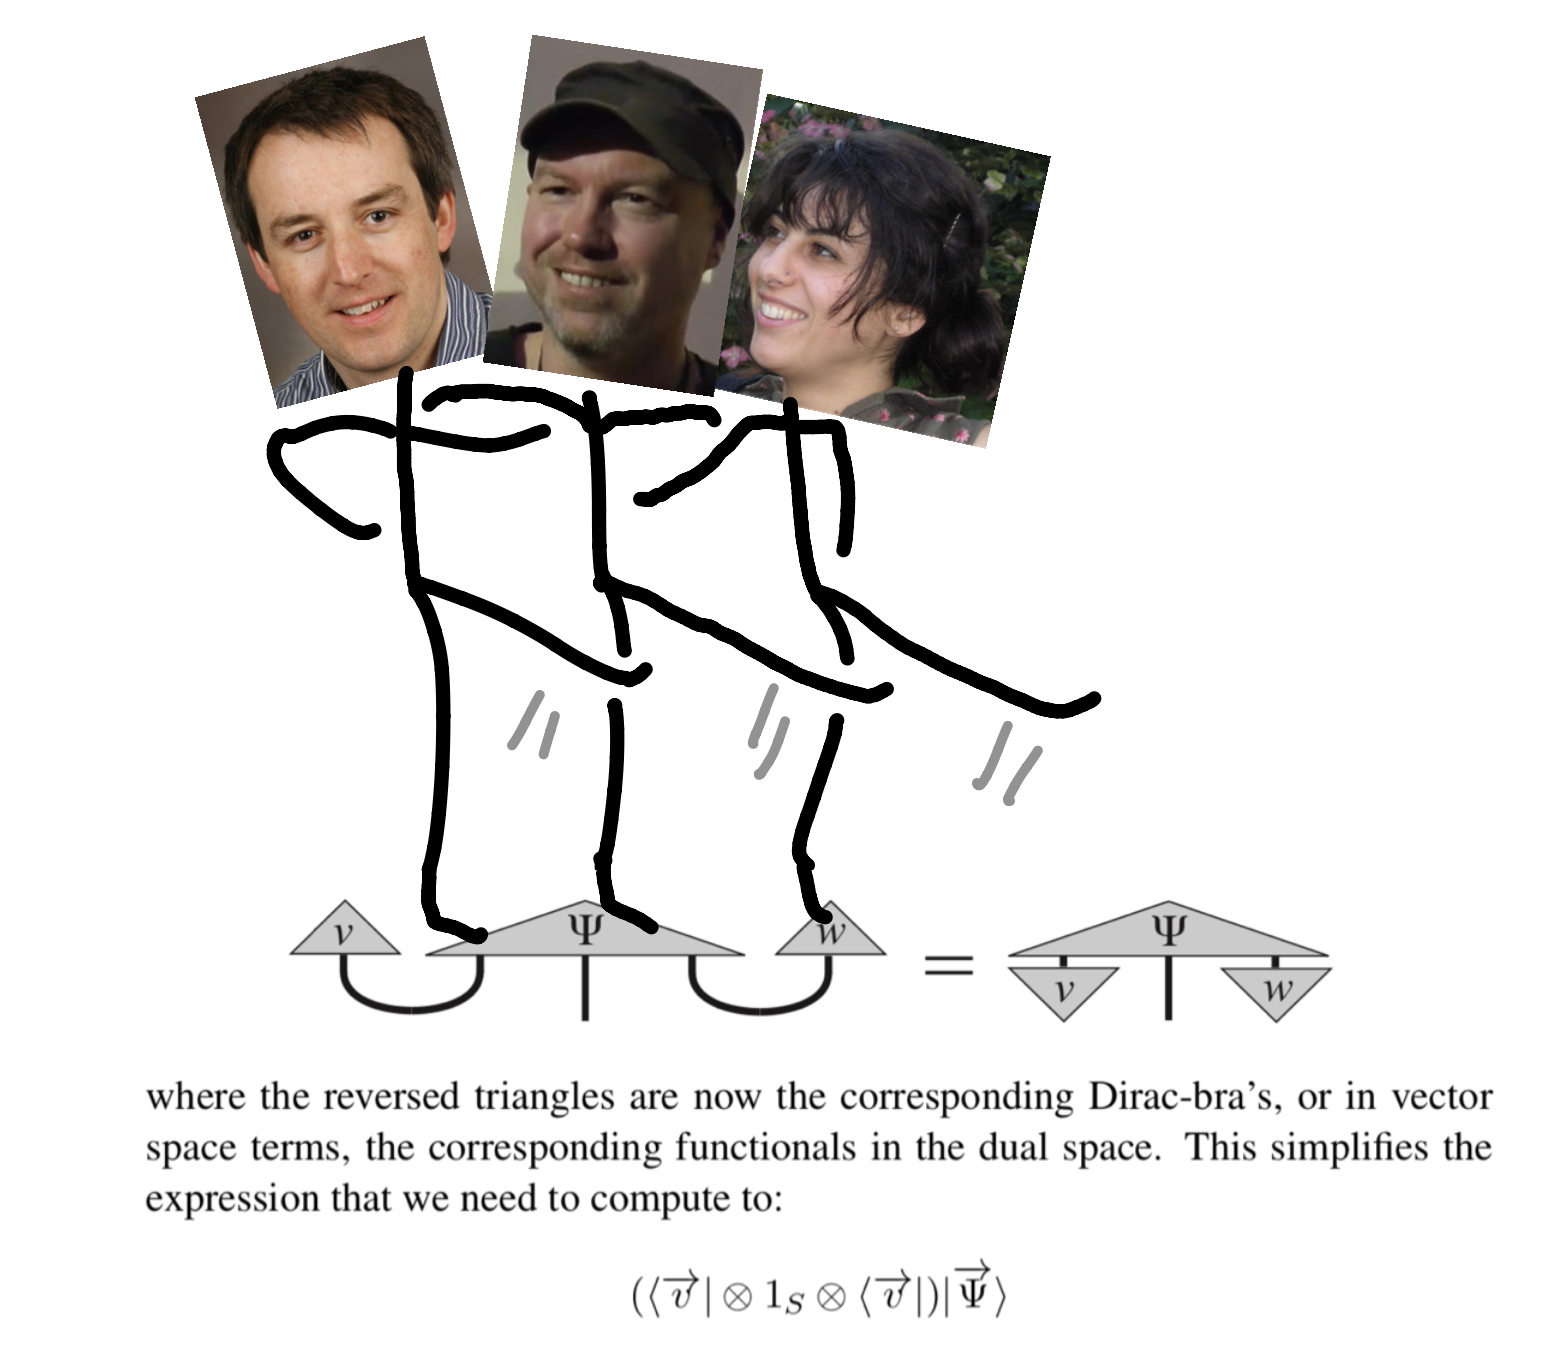
\includegraphics{figures/cartoons/disco1}}
\caption{Steve Clark was a professor in the computer science department at Oxford, and he was wondering how to compose vector-based semantic representations. Steve asked Bob, who realised suddenly what Jim was talking about. Mediated by the linguistic expertise of Mehrnoosh who was a postdoctoral researcher in Oxford at the time, pregroup diagrams were born. The basic types $n$ and $s$ are assigned finite-dimensional vector spaces, concatenation of types the kronecker product $\otimes$, and by the isomorphism of dual spaces in finite dimensions there is no need to keep track of the left- and right- inverse data. Words become vectors, and pregroup reductions become bell-states, or bell-measurements, depending on whether one reads top-down or bottom-up. There was simply no other game in town for an approach to computational linguistics that combined linguistic compositionality with distributional representations.}
\end{figure}

\begin{figure}[h!]
\centering
\scalebox{1}{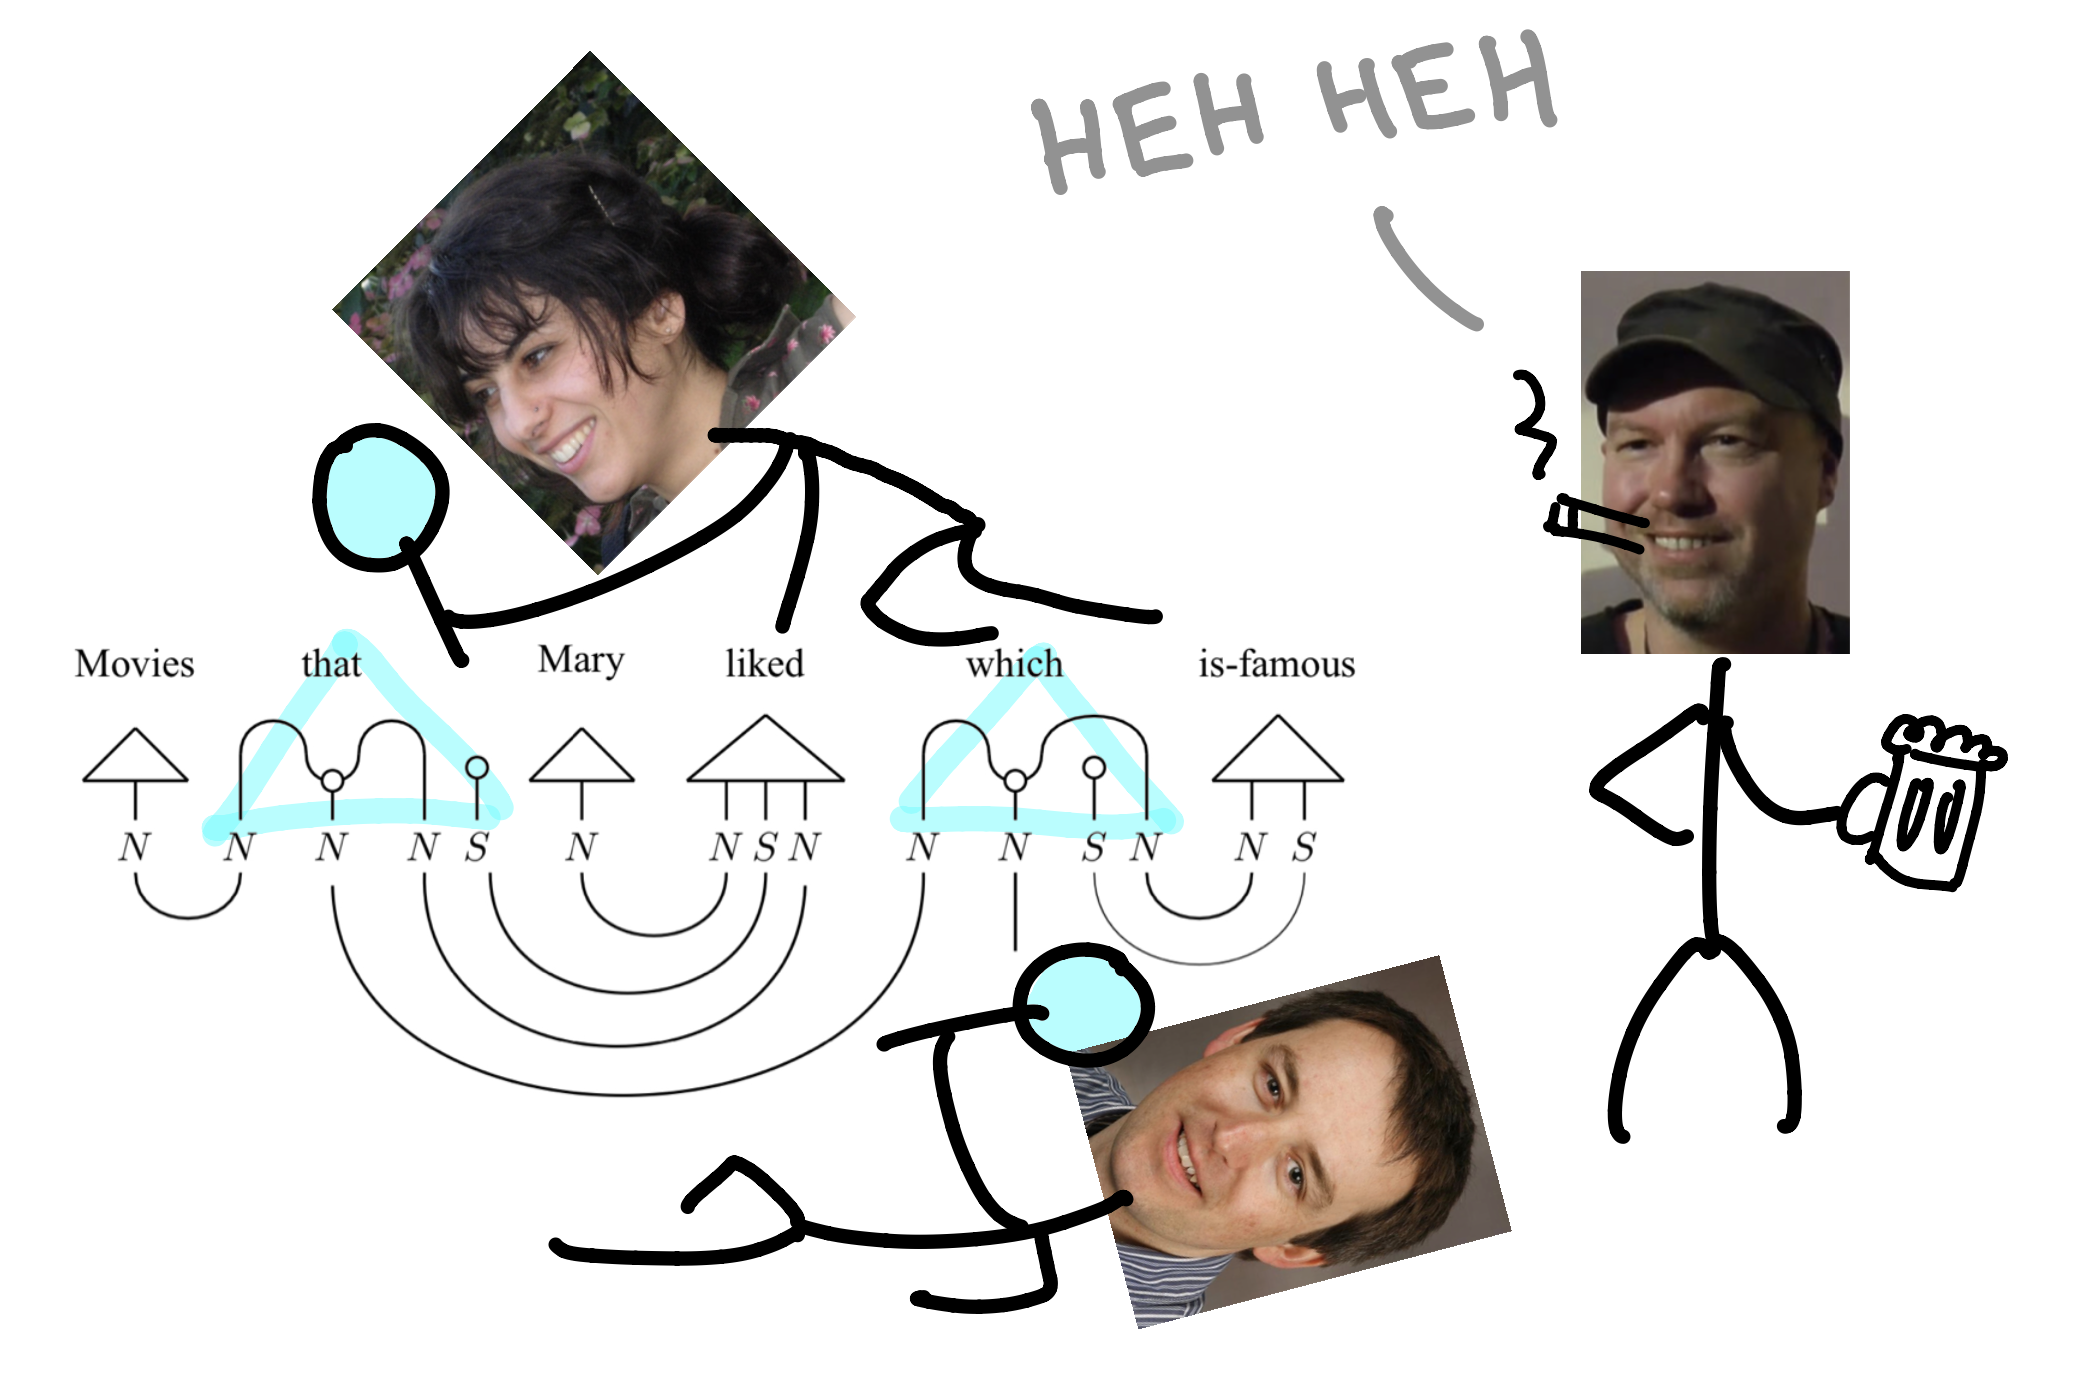
\includegraphics{figures/cartoons/disco2}}
\caption{In \emph{the frobenius anatomy of relative pronouns}\bR CITE \e, the trio realised that spiders could play the role of relative pronouns, which was genuinely novel linguistics. If one follows the noun-wire of "movies", one sees that by declaring the relative pronoun to be a vector made up of a particular bunch of spiders-as-multiwires, "movies" is copied to be related to the "liked" word, copied again by "which" to be related to the "is-famous" word, and a third time to act as the noun in the whole noun-phrase. This discovery clarified a value proposition: insights from quantum theory could be applied in the linguistic setting, and linguistics offered a novel use-case for quantum computers. For example, density matrices were used to model semantic ambiguity \bR CITE \e, and natural language experiments were performed on real quantum computeres \bR CITE \e.}
\end{figure}

\begin{figure}[h!]
\centering
\scalebox{1}{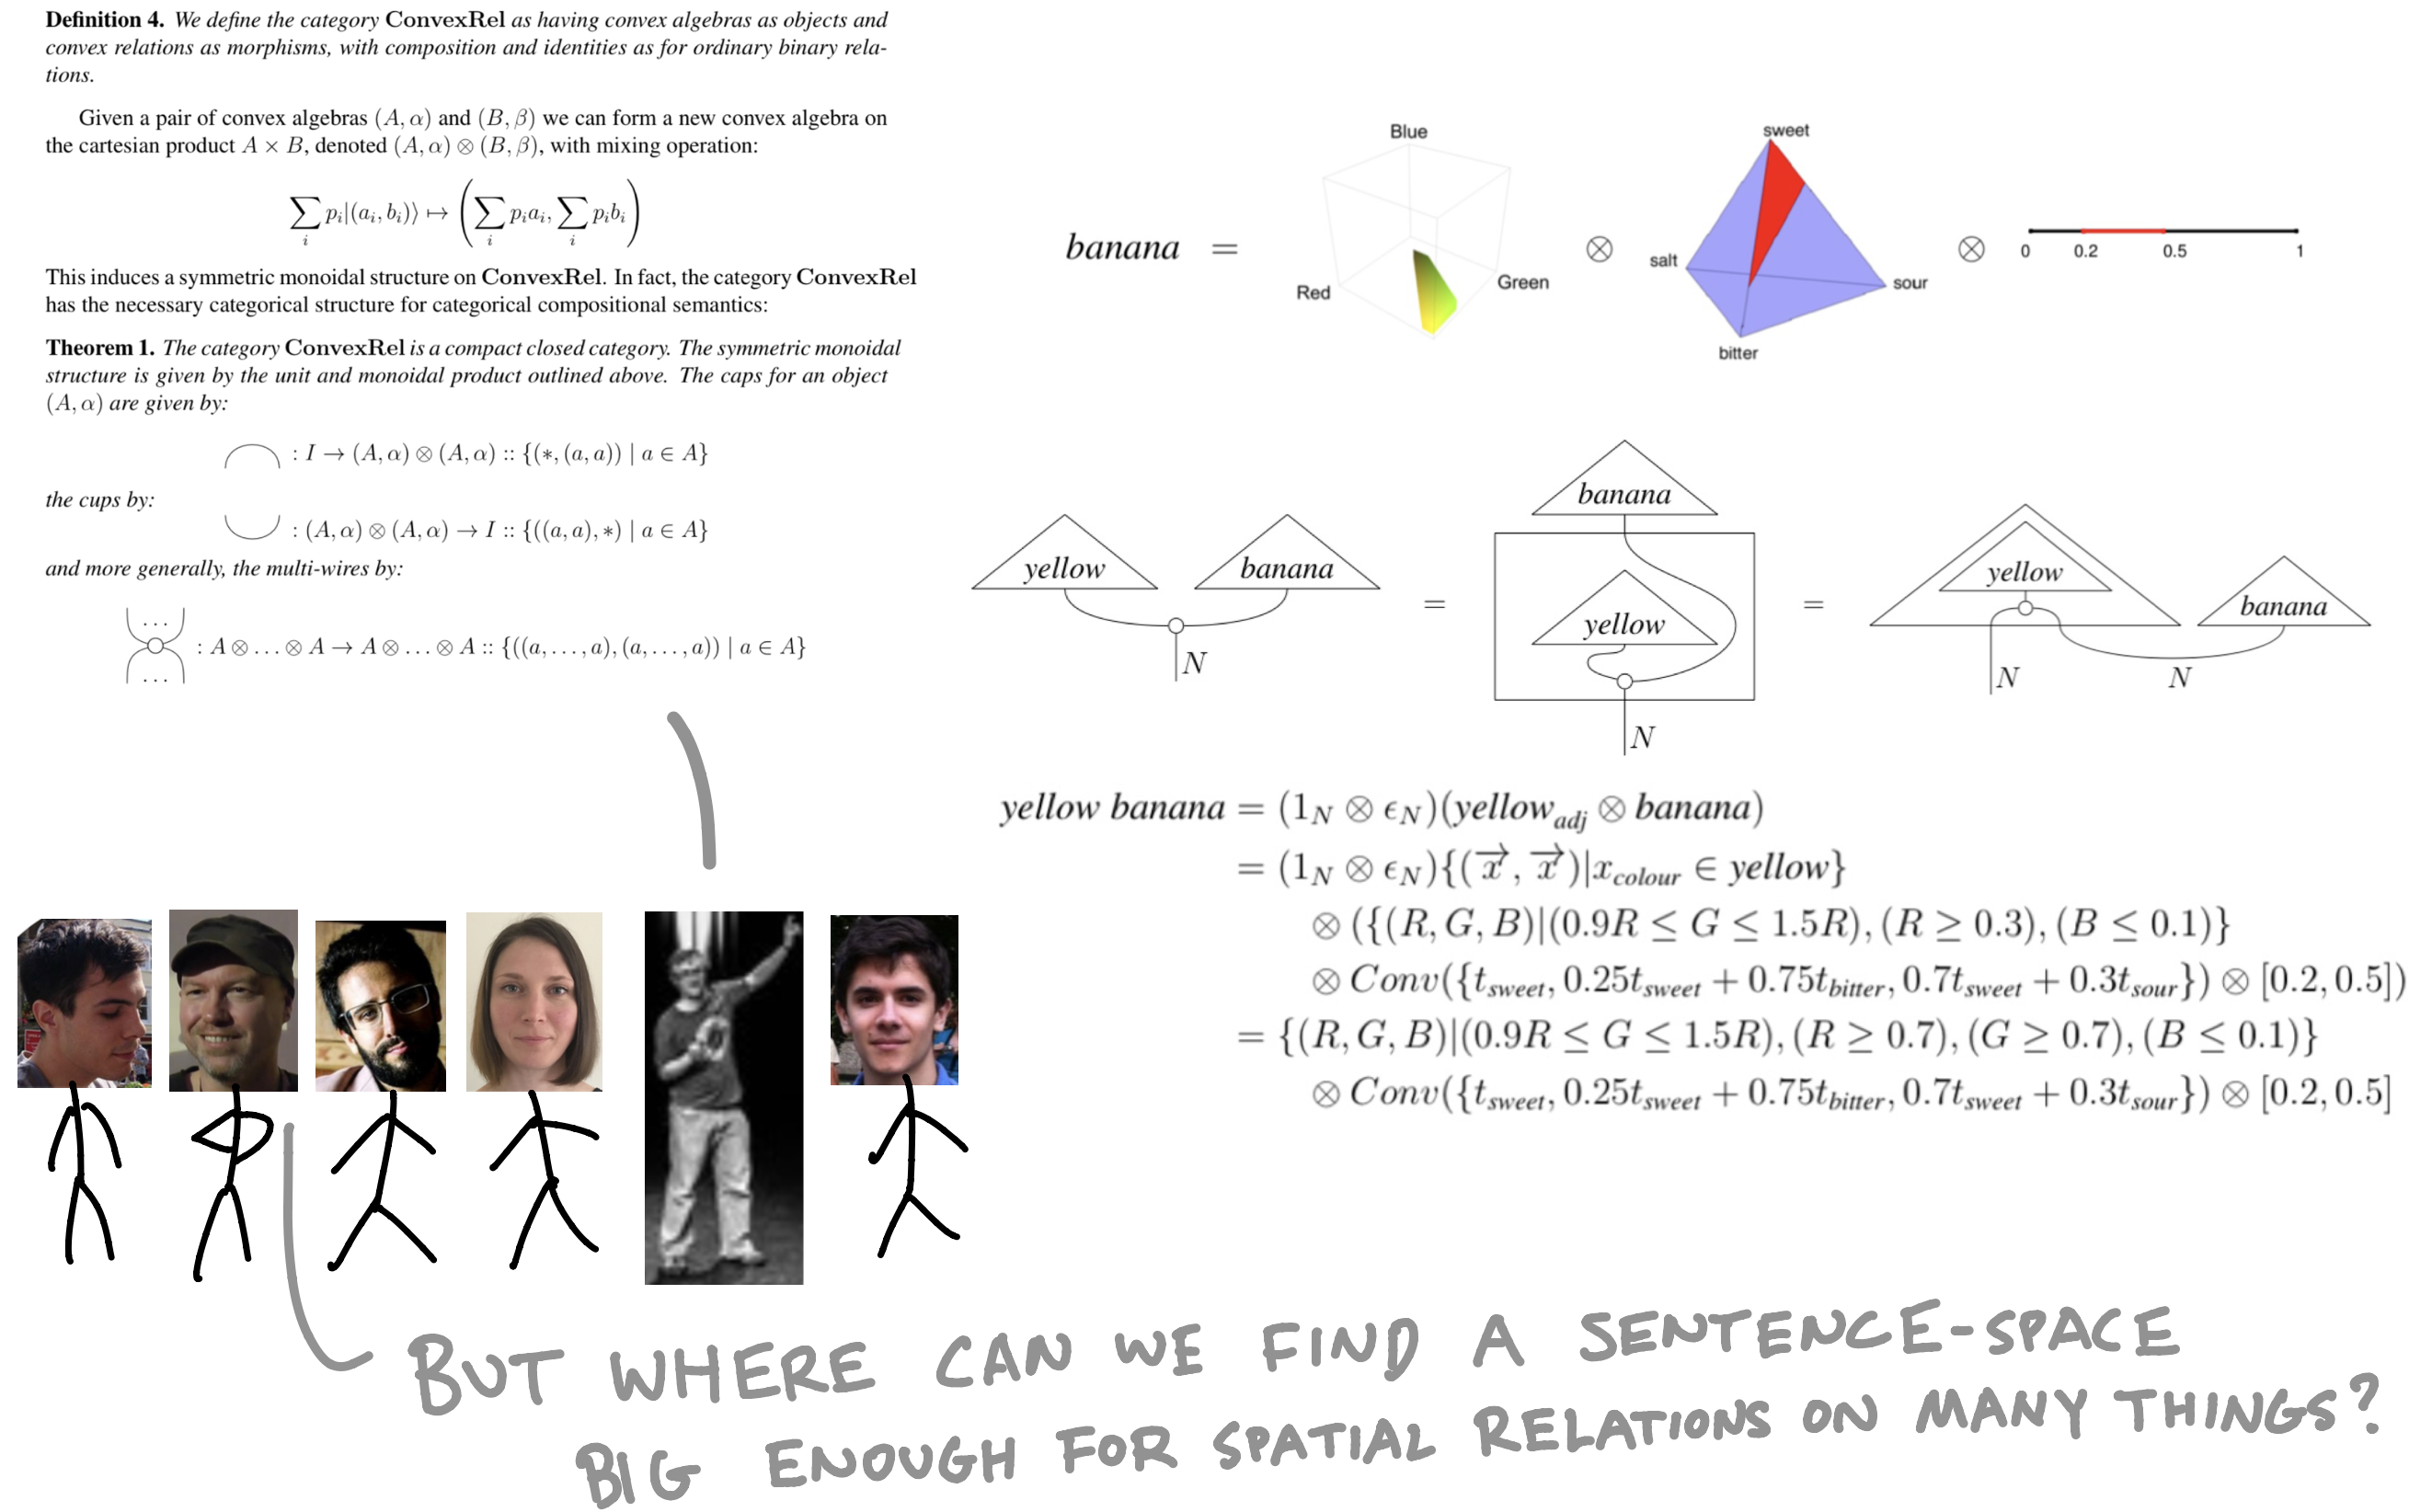
\includegraphics{figures/cartoons/disco3}}
\caption{Keeping the structure of the diagrams but seeking set-relational rather than vector-based semantics, a bridge was made between linguistics and cognitive science in \emph{interacting conceptual spaces I}\bR CITE \e. Briefly, G\"{a}rdenfors posits that spatial representations of concepts mediate raw sense data and symbolic representations -- e.g. red is a region in colourspace -- and moreover that concepts ought to be spatially convex -- e.g. mixing any two shades of red still gives red. This paper created a new point in the value proposition: that new mathematics would arise from investigating the linguistic-quantum bridge, e.g. generalised relations \bR CITE \e. Although labelled as if it is the first in a series, the paper never saw a sequel by the same title, blocked by an apparently simple but actually tricky theoretical problem. The problem is that while this convex-relational story worked for conceptual adjectives modifying a single noun such for "sweet yellow bananas", there was difficulty in extending the story to work for multiple objects interacting in the same space, as in "cup on table in room". It couldn't be worked out what structure a sentence-wire in \textbf{ConvexRel} ought to have in order to accommodate (in principle) arbitrarily many objects and spatial relations between them.\\

DisCoCat then diverges from the story I want to tell. In no particular order, QNLP was done on an actual quantum computer \bR CITE \e, some software packages were written \bR CITE \e, and some art was made \bR CITE \e.}
\end{figure}
\clearpage



\subsection{I killed DisCoCat, and I would do it again.}

\begin{figure}[h!]
\centering
\scalebox{1}{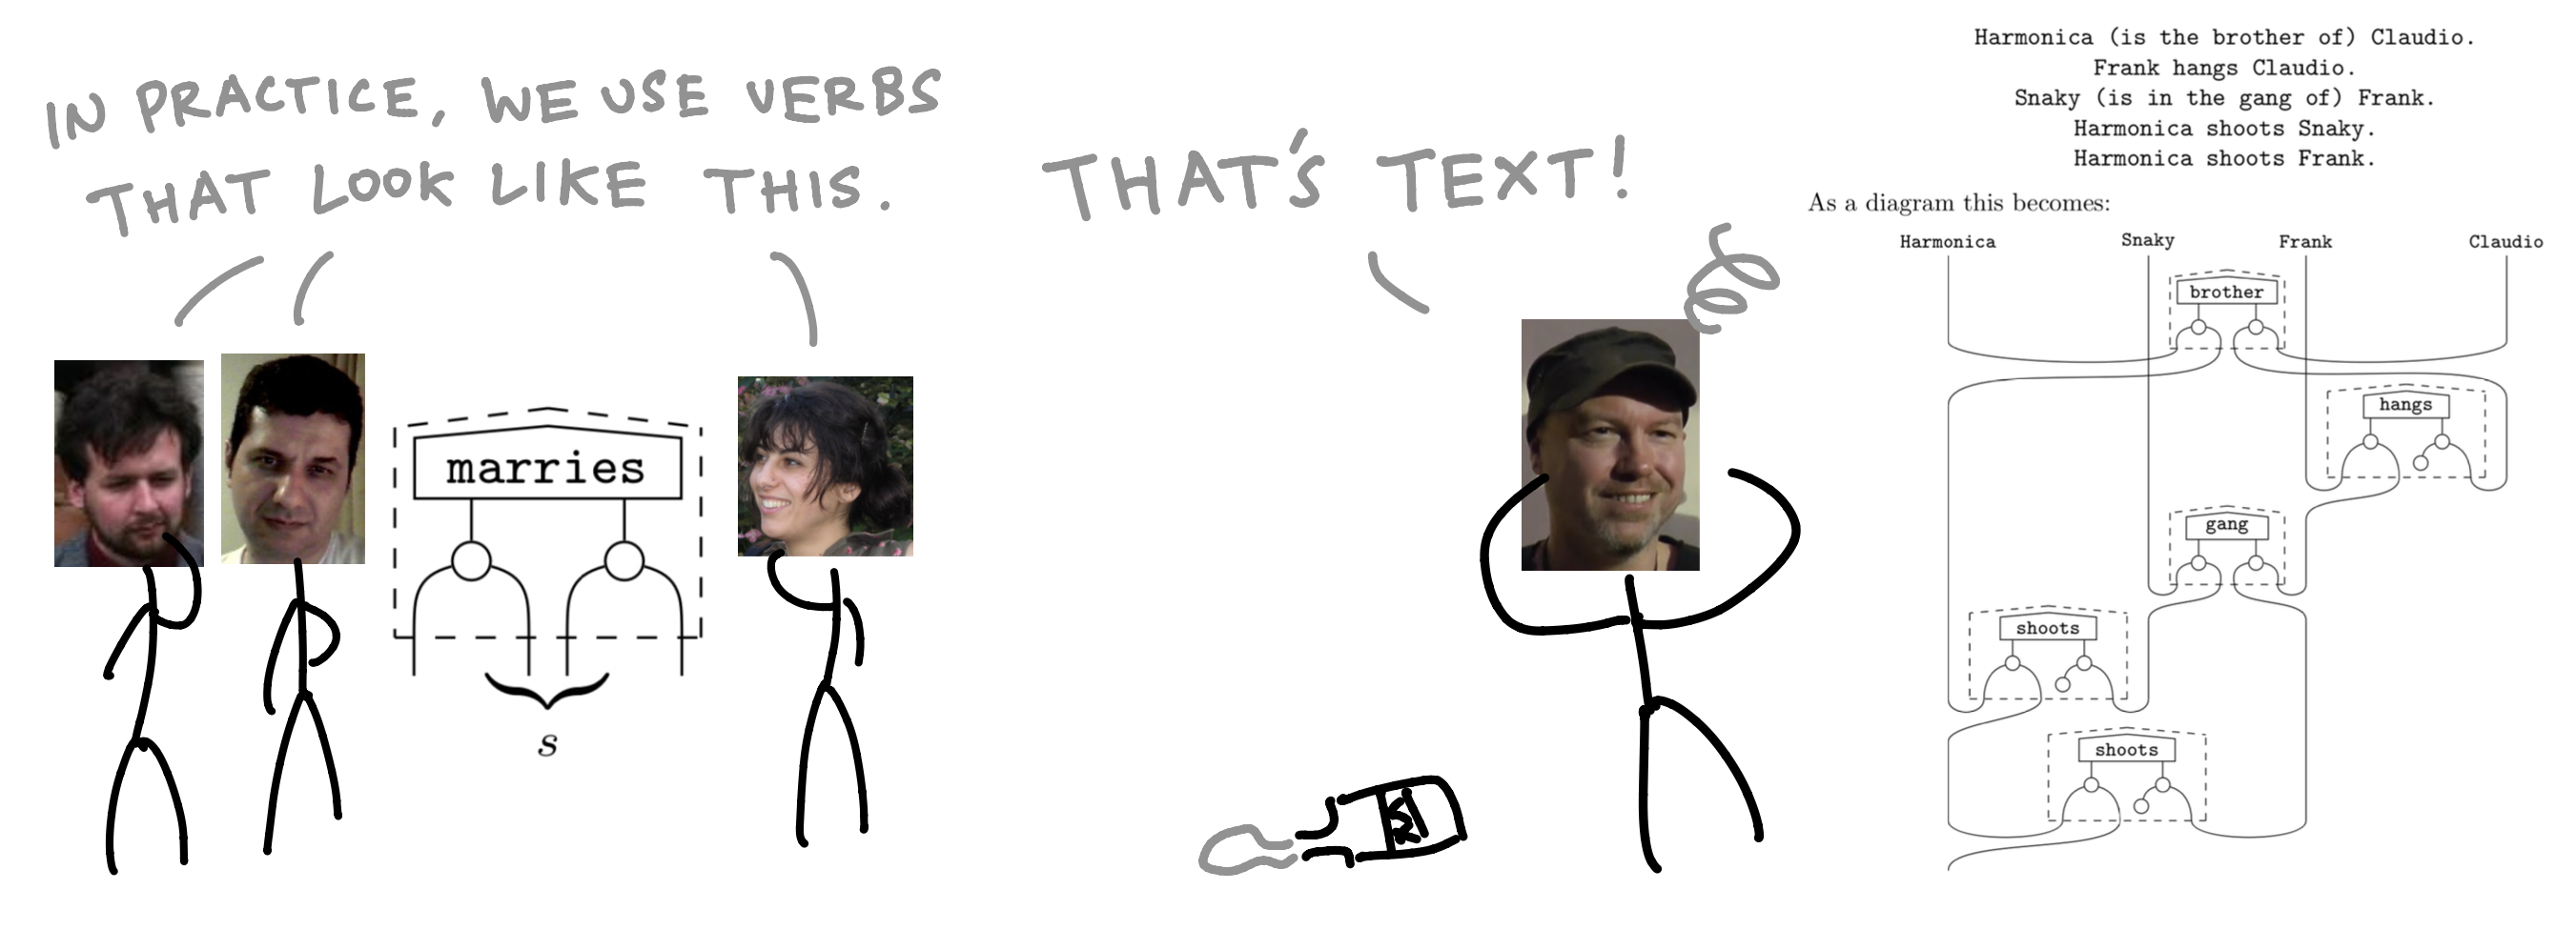
\includegraphics{figures/cartoons/discocirc1}}
\caption{It is a common evolutionary step in linguistics that theories `break the sentential barrier', moving from sentence-restricted to text- or discourse-level analysis \bR CITE \e. The same thing happened with DisCoCirc, due to a combination of practical constraints and theoretical ambition. On the practical side, wide tensors were (and remain) prohibitively expensive to simulate classically and actual quantum computers did not (and still do not) have many qubits, hence in practice pregroup diagrams were reduced to thinner and deeper circuits, often with the help of an additional simplifying assumption that sentence wires were pairs of noun wires in the illustrated form on the left. Theoretically, seeking dynamic epistemic logic, Bob had an epiphanous hangover (really) where he envisioned that these "Cartesian verbs" could be used in service of compositional text meanings, and he called this idea DisCoCirc \bR CITE \e.}
\end{figure}

\begin{figure}[h!]
\centering
\scalebox{1}{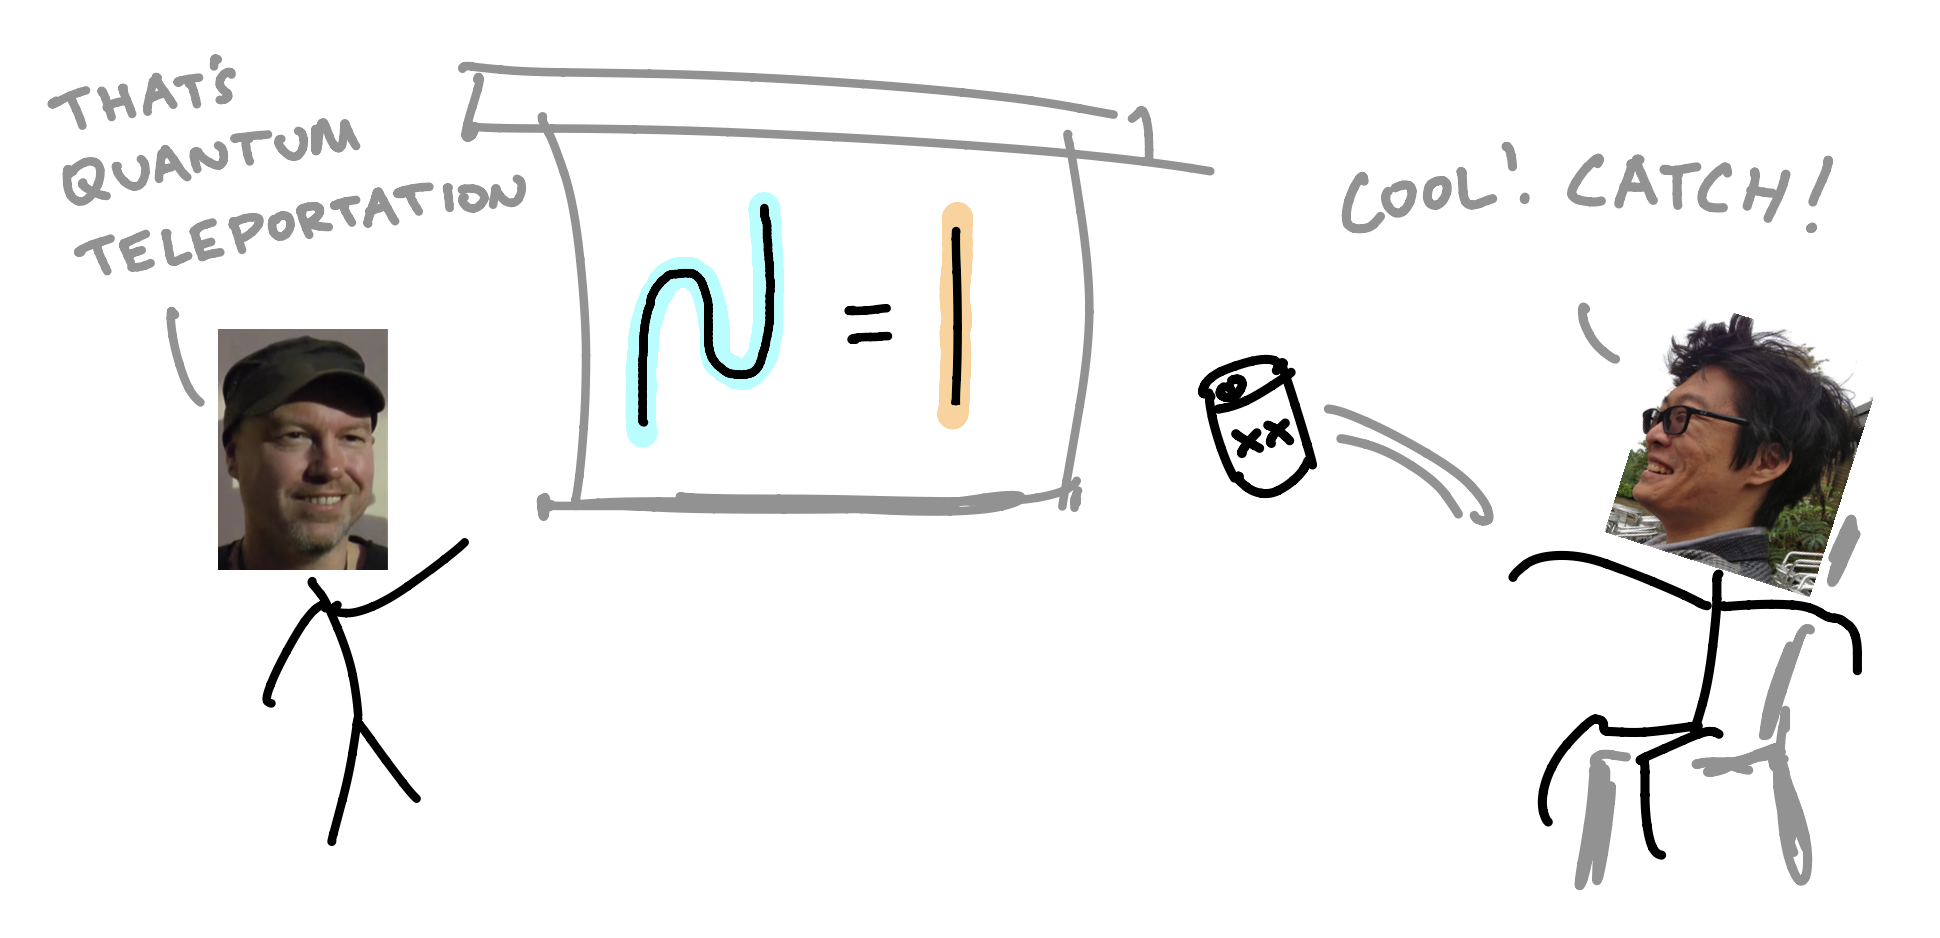
\includegraphics{figures/cartoons/v1}}
\caption{I met Bob in my master's in 2019, where he taught the picturing quantum processes course. When quantum teleportation was explained in half a minute by a diagram, I decided to pursue a DPhil in diagrammatic mathematics. In the last lecture, I threw Bob a cider, after which he seemed to like me. I did not know he was an alcoholic.}
\end{figure}
\clearpage

I was shanghaied into thinking about diagrams for language. I was deeply dissatisfied with the content from the standpoint my own intellectual integrity. Firstly, there seemed to me an unspoken claim that the presence of cups in pregroup diagrams (which implied a noncartesian and hence large tensor product) made it necessary to use quantum computers to effectively compute pregroup diagrams. I just could not believe that my brain required quantum computation to understand language. This implicit claim of kinship between quantum and linguistics was further entrenched by the analysis of the relative pronoun in terms of frobenius algebras, since spiders in $\mathbf{Vect}^\otimes$ were the \emph{sine qua non} of categorical quantum mechanics. The best steelman for spiders I have is that frobenius algebras (which are central to bicategories of relations \bR CITE \e) just happen to be a ubiquitous mathematical structure that are well-suited to express the mathematics of connections, both in language and in quantum.\\

Second, representing the content of a sentence as a vector in a sentence-vector-space did not sit well with me, since this move meant that the only meaningful thing one could do with two sentences was take their inner-product as a measure of similarity. Moreover, I had the theoretical concern that language is in principle indefinitely productive, so one could construct a sentence that marshalled indefinitely many nouns, and at some point for any finite vector space $s$ one would run out of room to encode relationships, or else they would be cramped together in a way that did not suit intuitions about the freedom of constructing meanings using language. I always believed in the existence of a simple, practical, and intuitive categorical, compositional, and distributional semantics; I just didn't believe that the role of quantum -- however helpful or interesting -- was \emph{necessary}.

My first unsatisfactory attempt was in my Master's thesis \bR CITE \e. It had been known for a while that a free autonomous category construction by Delpeuch \bR CITE \e could potentially eliminate some of the cups in pregroup diagrams, yielding what amounted to a method to transform a pregroup diagram into a monoidal string diagram in the shape of a context-free grammar tree. This trick had the limitation that freely adding directed cups and caps to a string diagrammatic signature did not turn a symmetric monoidal category into a (weakly) compact closed one, rather just into a monoidal category where the original wires had braidings, but all the new left and right dual wires did not; this presented difficulties in accounting for iterated duals for higher-order modifiers such as adverbs in grammatical types, and had nothing to say about spiders. I tried to generalise this trick to `freely' adding arbitrary diagrammatic gadgets to string diagrams, but my assessor Samson pointed out that it was nontrivial to determine whether such constructions were faithful. In retrospect the free autonomous completion of a parameterised \bR CITE \e markov category \bR CITE \e is in the ballpark of dequantumfying pregroup diagrams, but I didn't learn about them until later, and that still wouldn't have addressed the issues that come with only having a sentence-wire.

\begin{figure}[h!]
\centering
\scalebox{1}{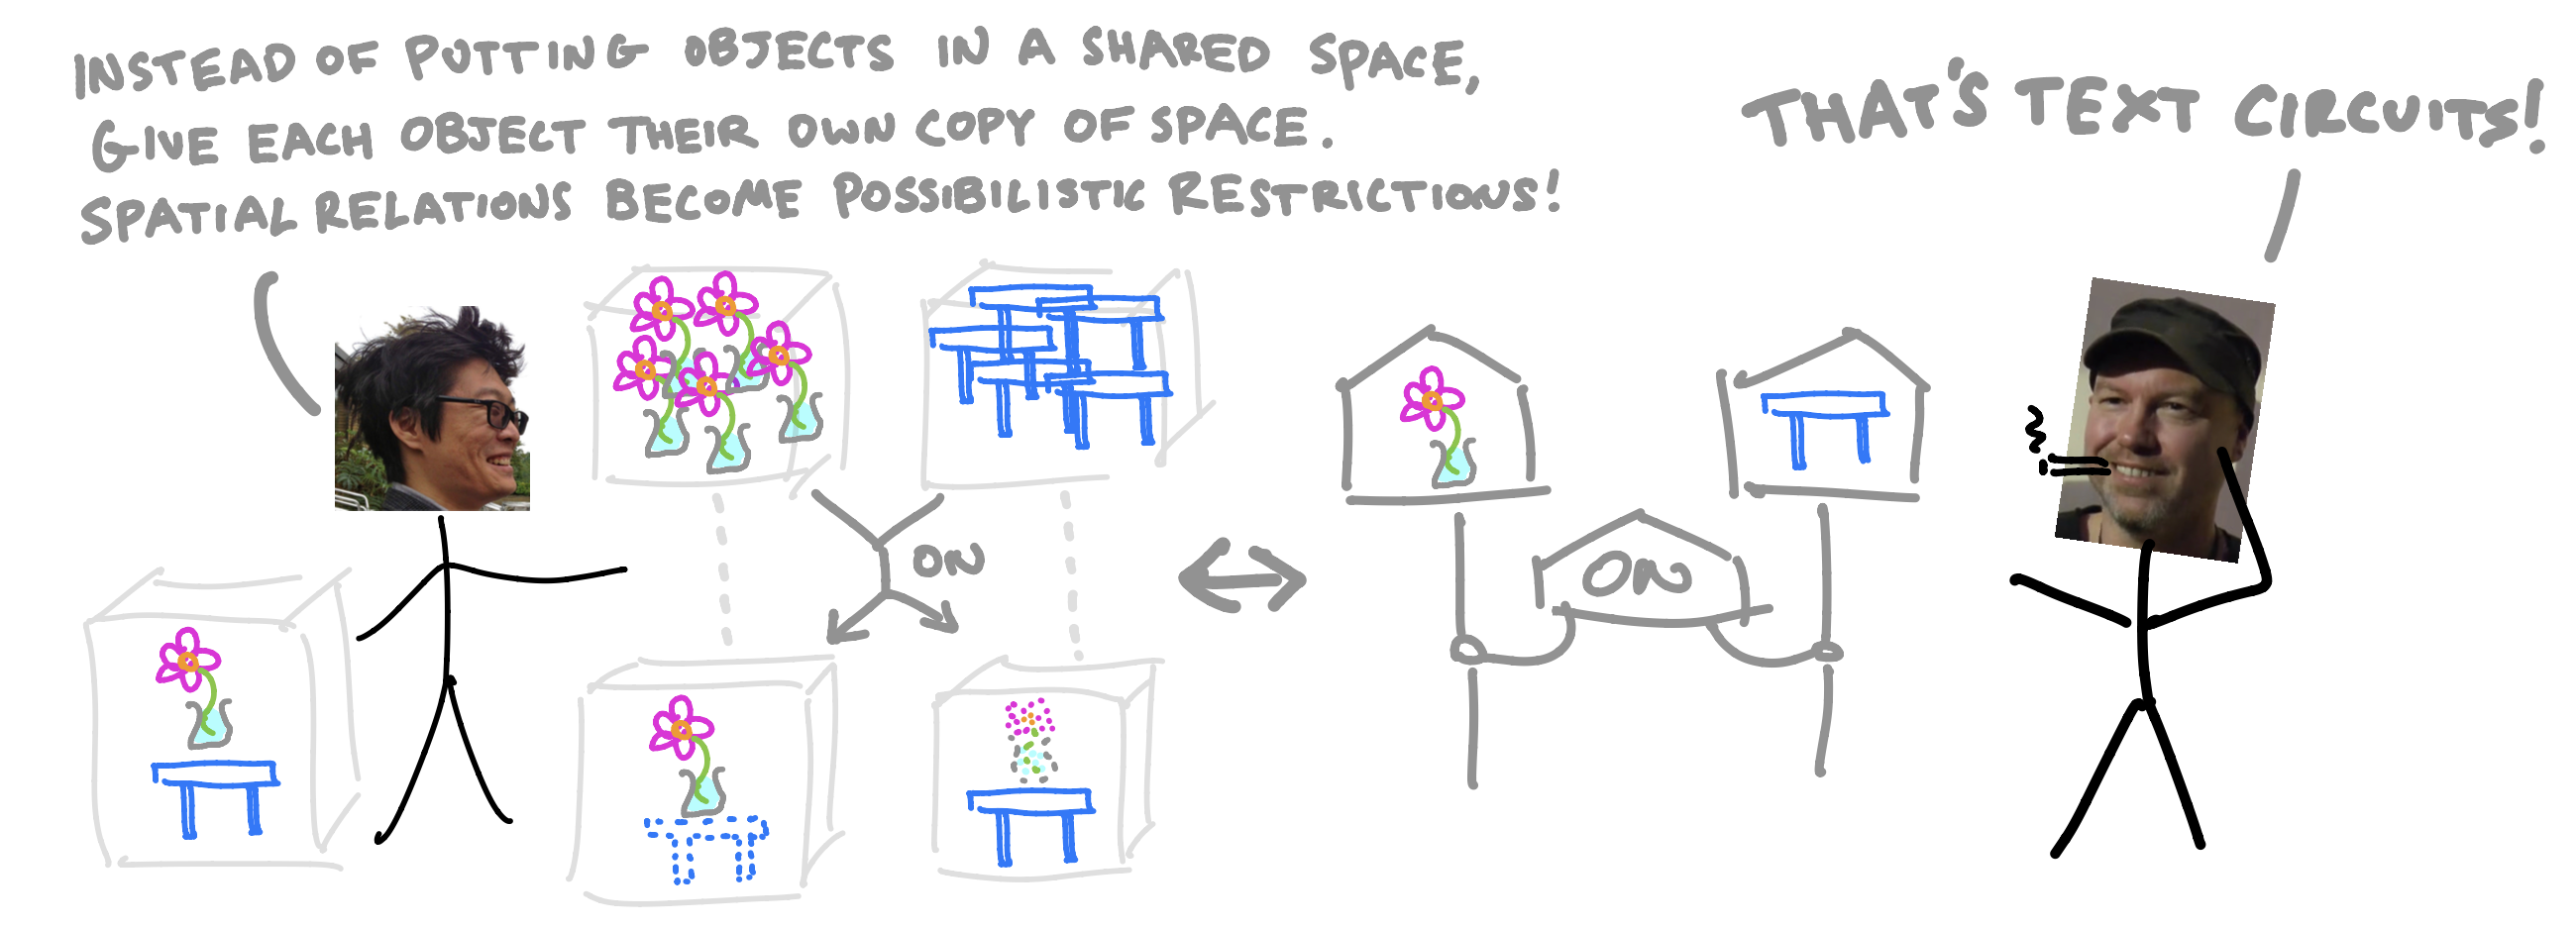
\includegraphics{figures/cartoons/circify1}}
\caption{Then COVID happened. During the first lockdown, I visited Bob's garden under technically legal circumstances, and I suggested a solution to the longstanding problem of representing linguistic spatial relationships. My theoretical concern was the culprit: the initial attempts at the problem failed because the approach was to find a single sentence object $s$ in which one could paste the data of arbitrarily many distinct spatial entities. The simple solution was a change in perspective.}
\end{figure}

\begin{figure}[h!]
\centering
\scalebox{1}{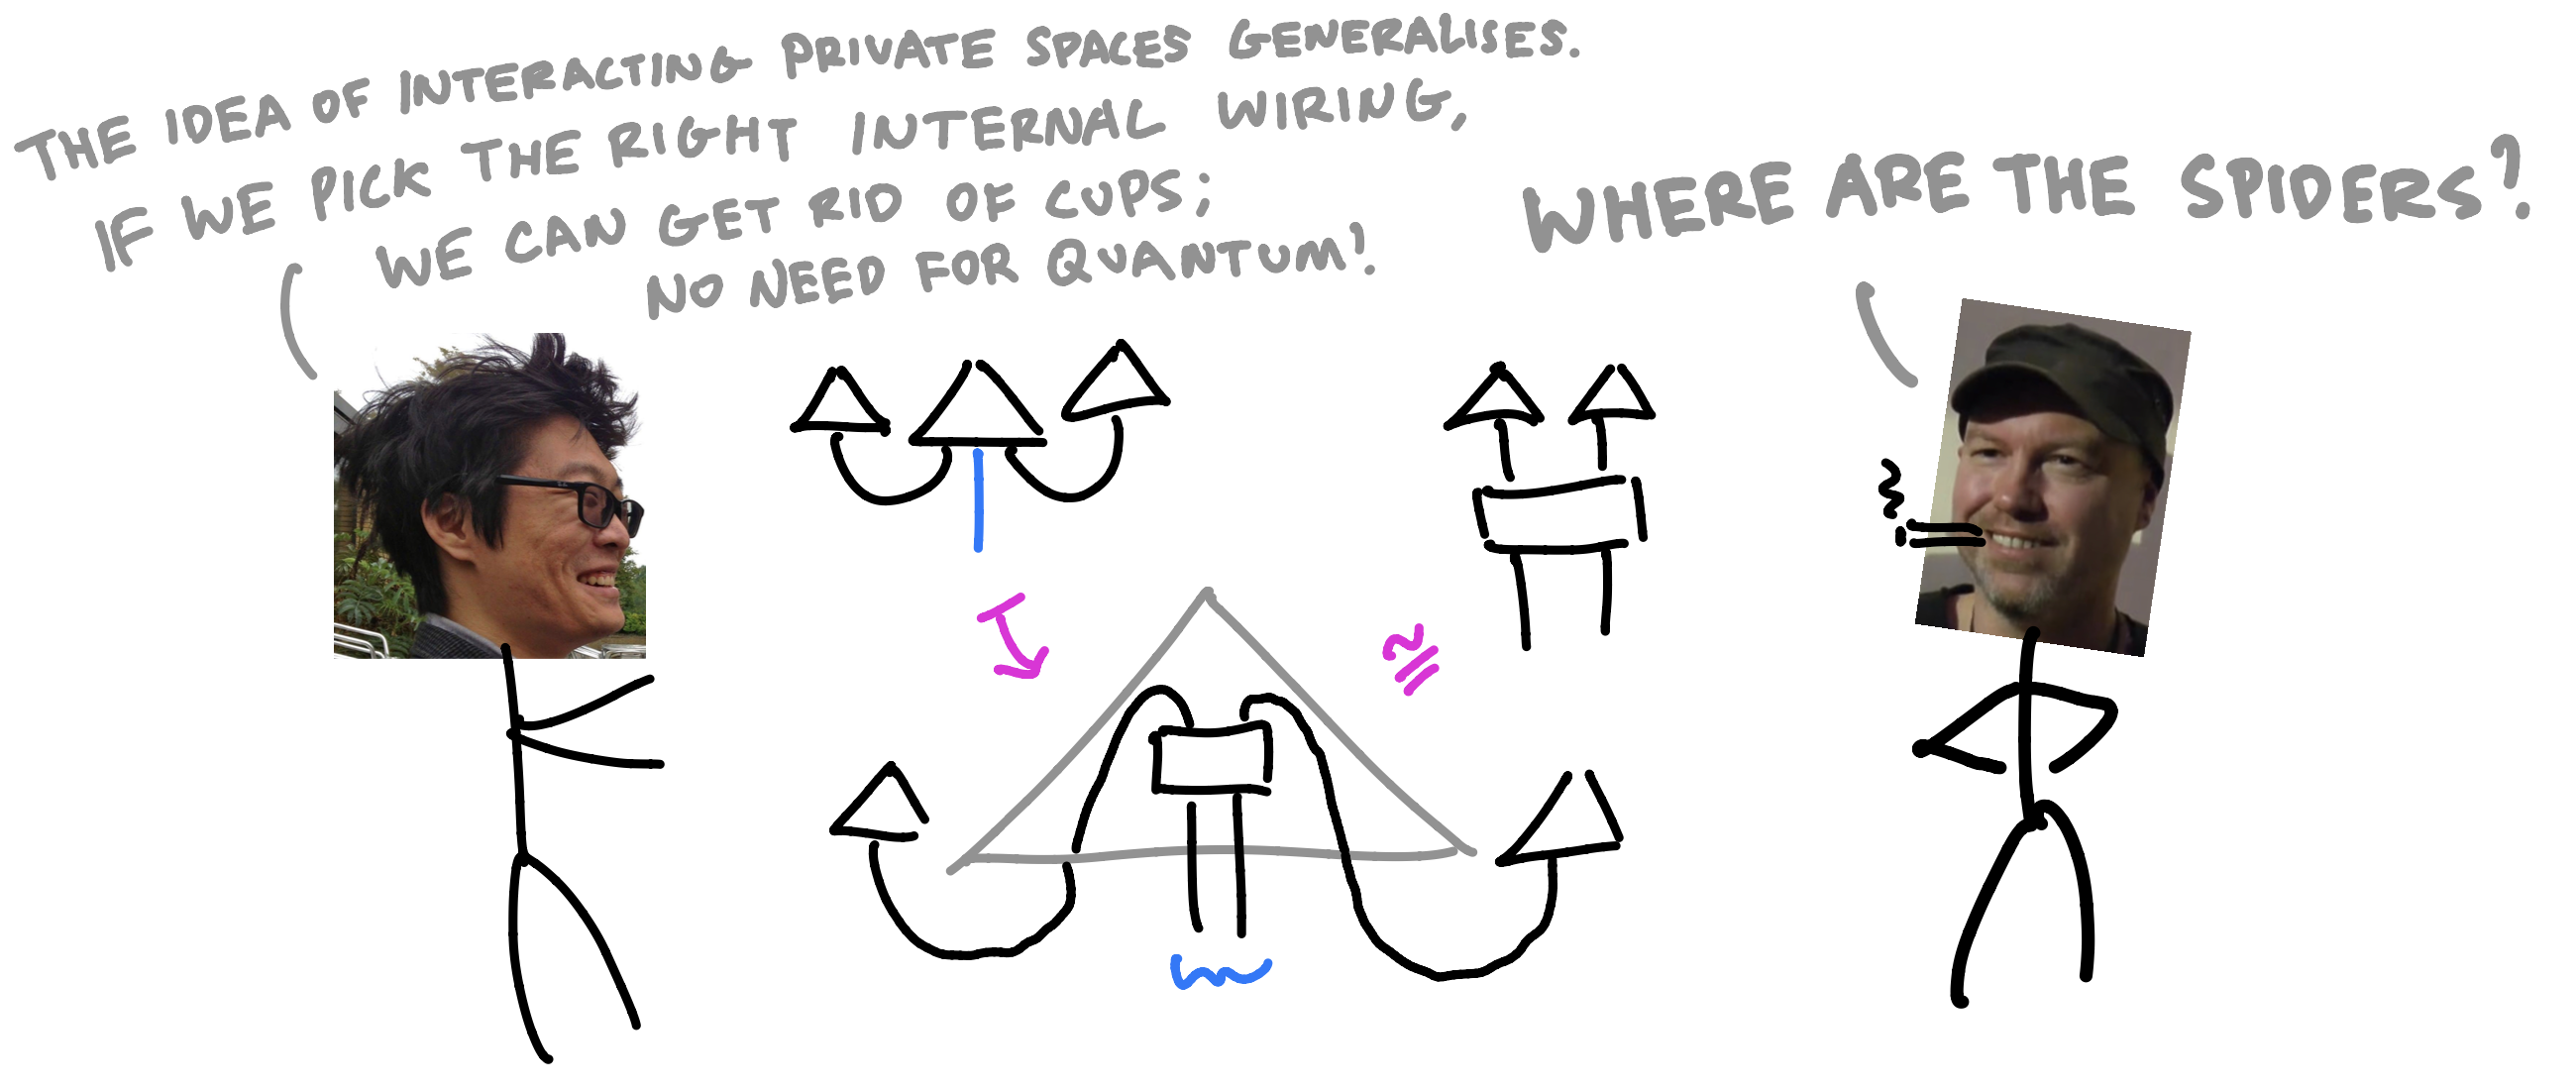
\includegraphics{figures/cartoons/circify2}}
\caption{That this move of splitting up the sentence-wire into a sentence-dependent collection of wires was sufficient to solve what had appeared to be a difficult problem prompted some re-examination of foundations. The free autonomisation trick in conjunction with sentence-wire-as-tensored-nouns seemed promising, but it became clear that right way to drown a DisCoCat thoroughly was to explain and eliminate the spiders.}
\end{figure}

\begin{figure}[h!]
\centering
\scalebox{1}{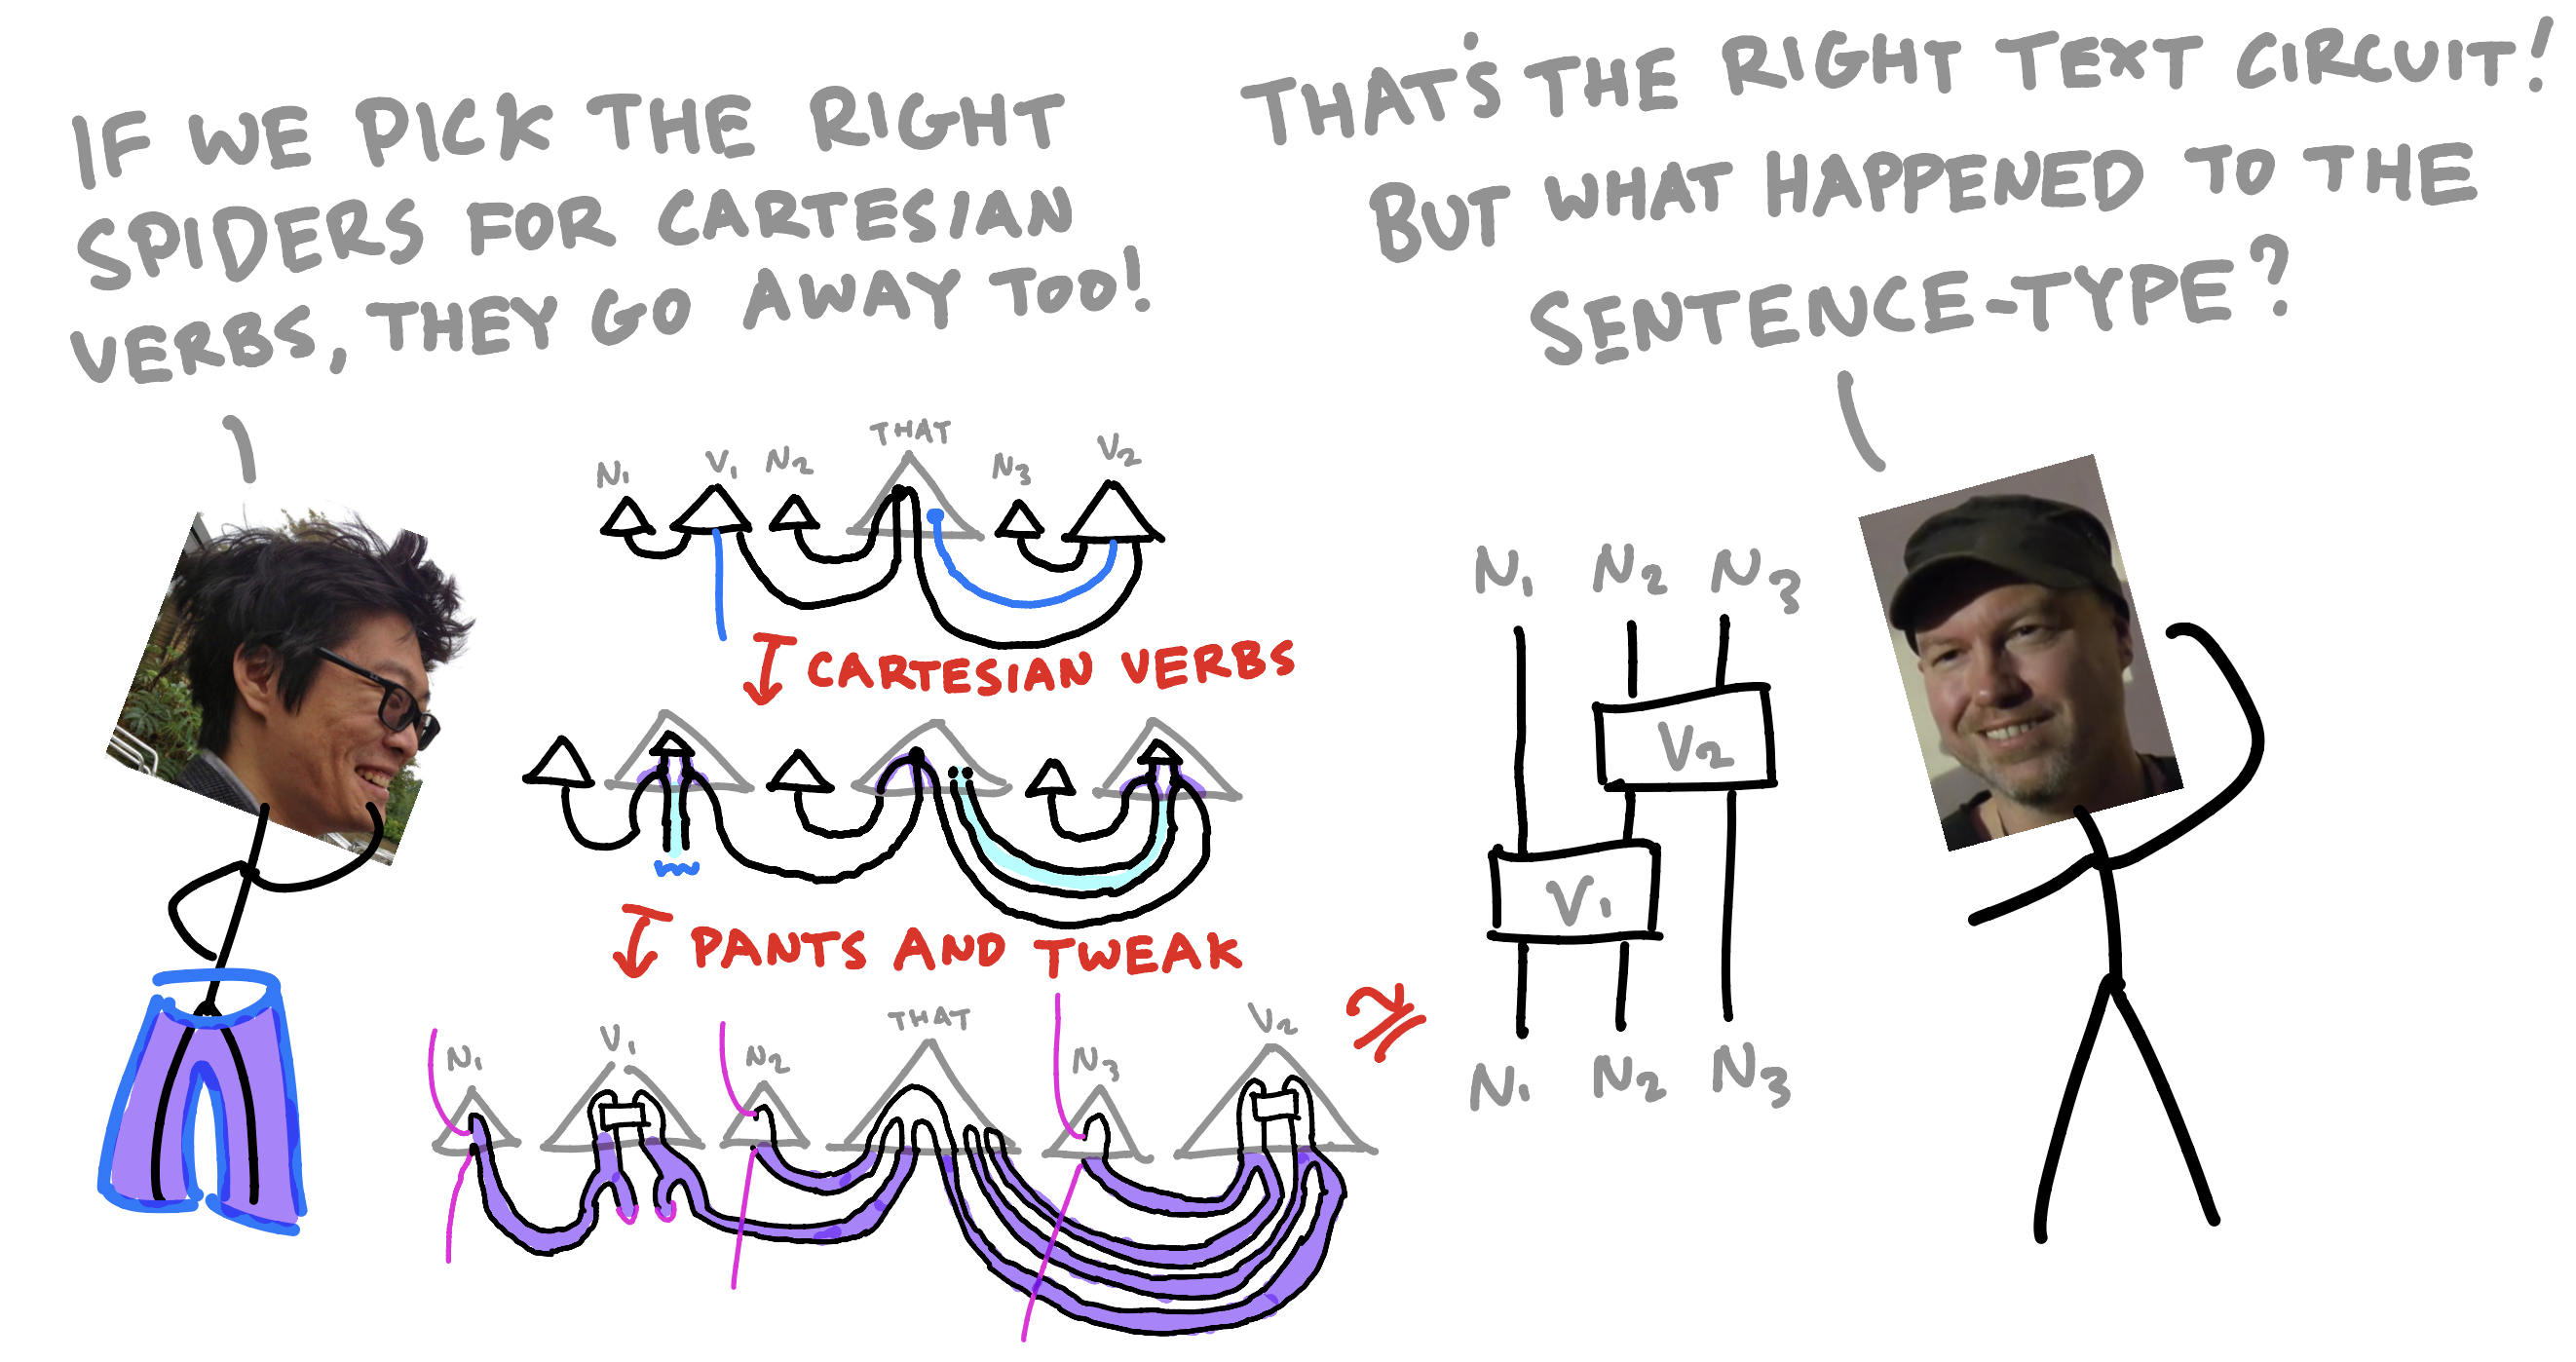
\includegraphics{figures/cartoons/circify3}}
\caption{I then discovered that by interpreting spiders as the well-known "pair of pants" algebra in a compact closed monoidal setting allowed for a procedure in which the final form was purely symmetric monoidal -- the absence of cups and caps meant that there was no practical necessity to interpret diagrams on quantum computers: \emph{any} computer would suffice. The role of spiders for relative pronouns was illuminated in the presence of splitting the sentence wire: the pair-of-pants are the algebra of morphism composition, and splitting the sentence wire into a collection of nouns allowed relative-pronoun-spiders to pick out the participating nouns to compose relationships onto.}
\end{figure}

\begin{figure}[h!]
\centering
\scalebox{1}{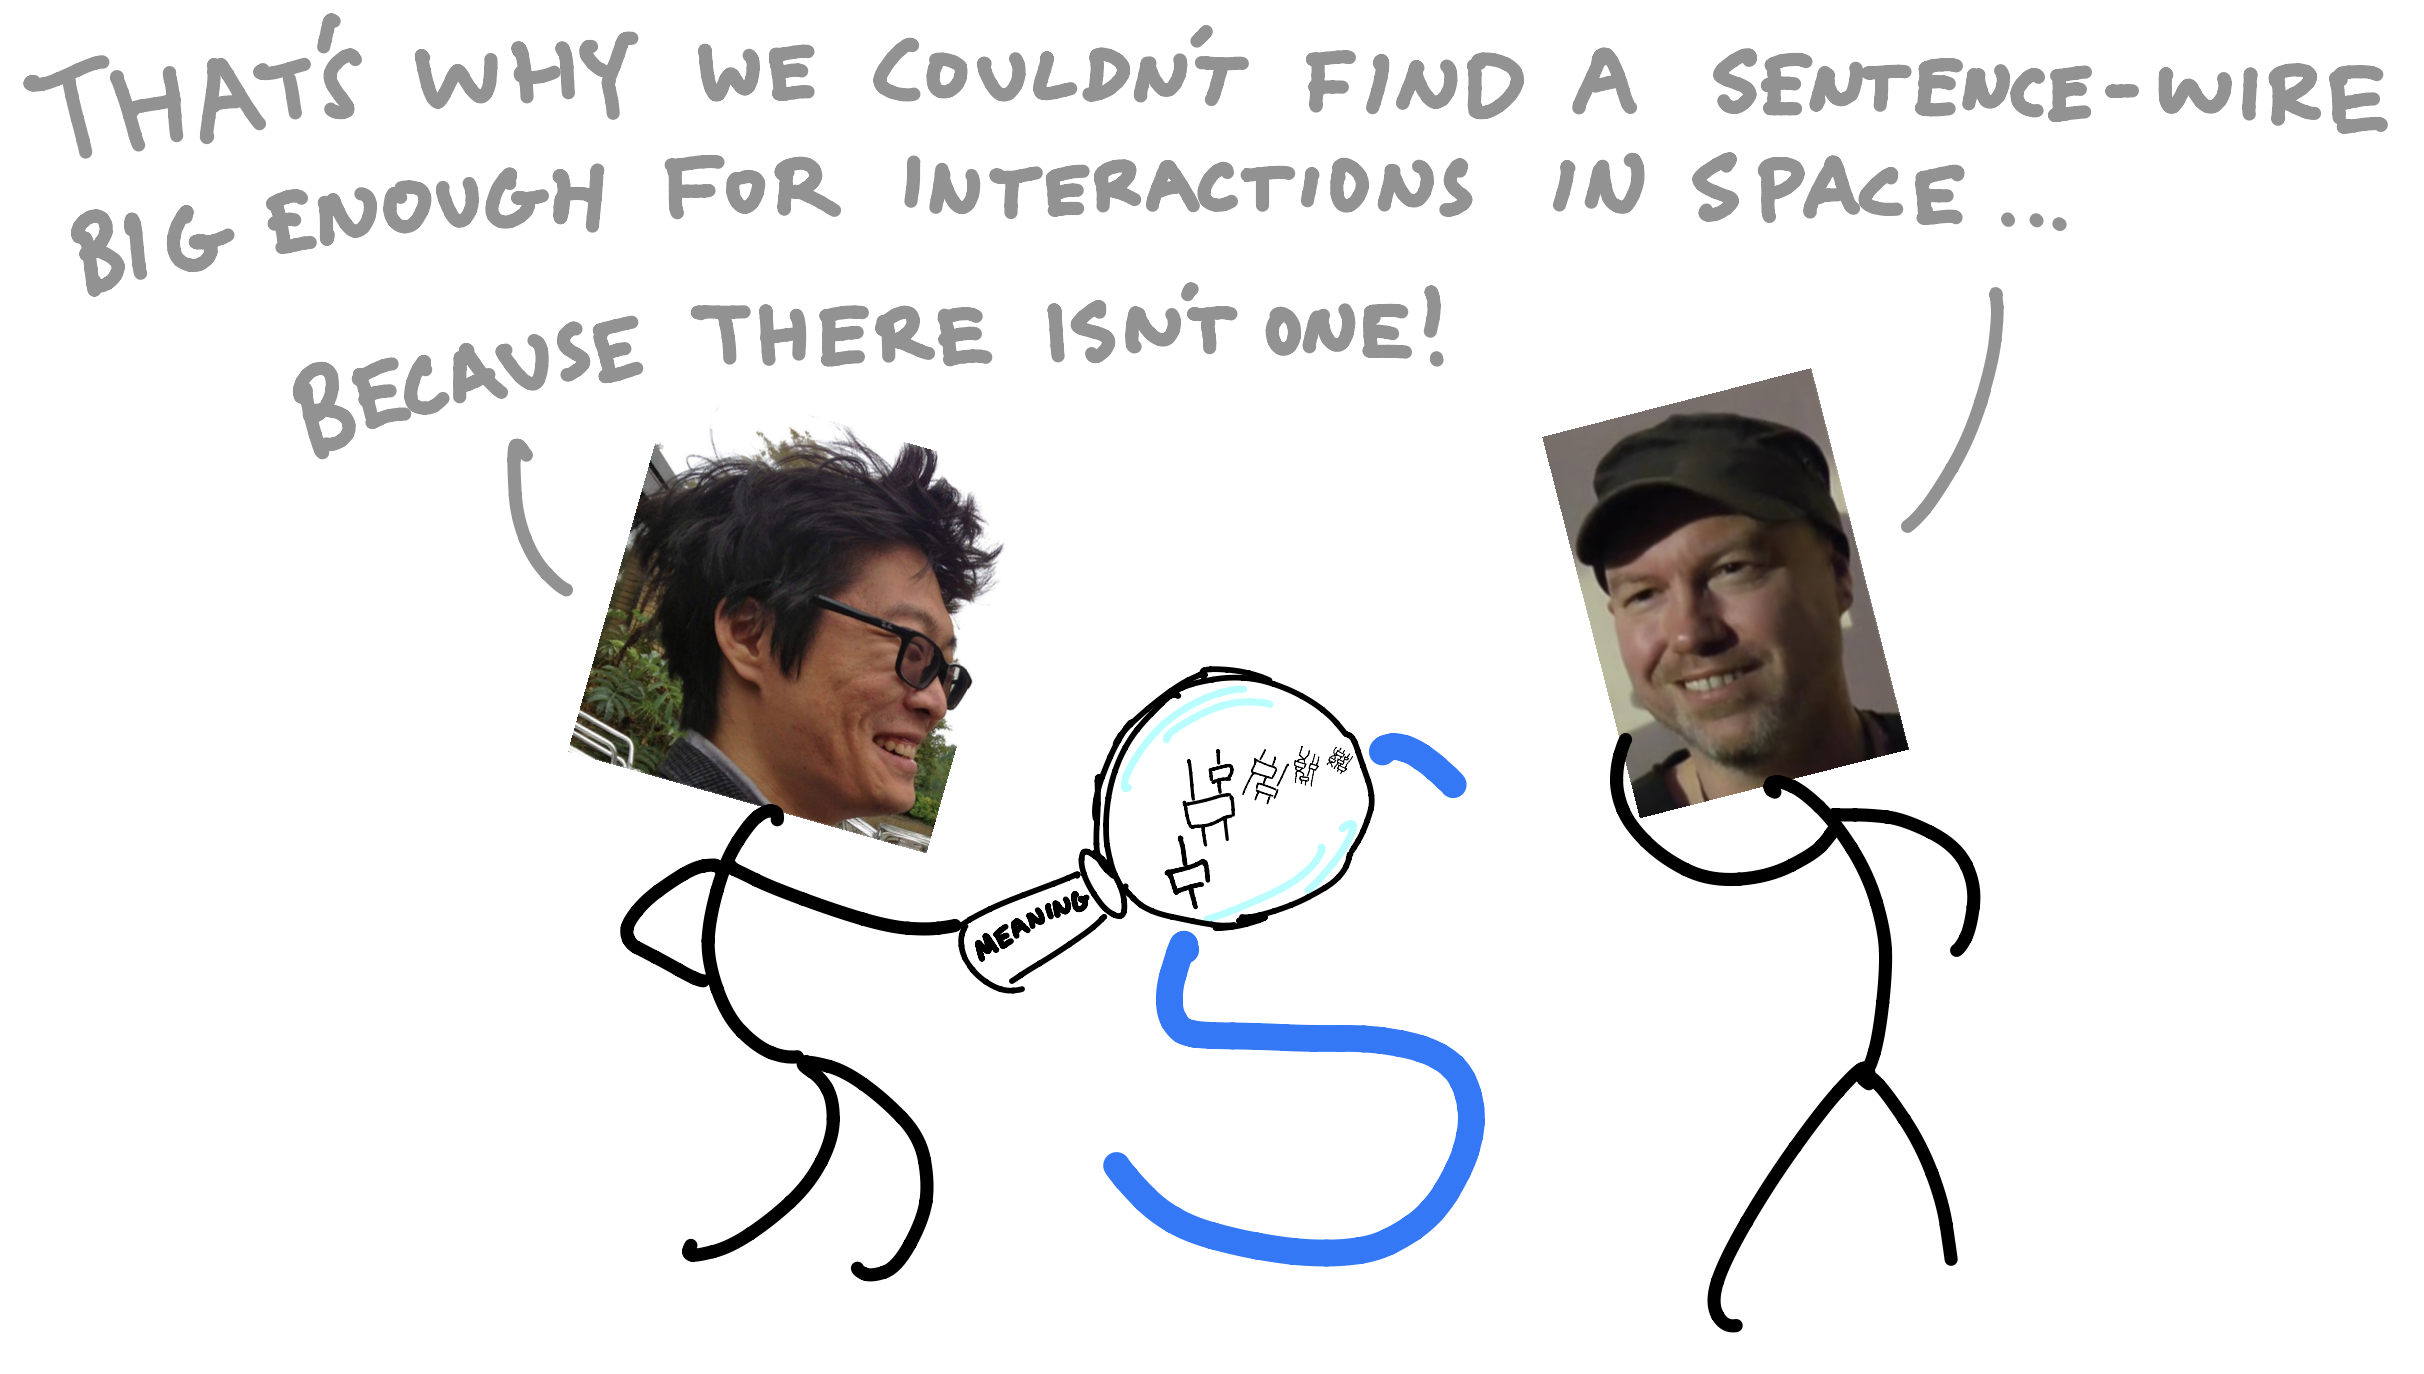
\includegraphics{figures/cartoons/nosent}}
\caption{A coherent conservative generalisation of DisCoCat with less baggage had emerged, or rather, DisCoCirc was placed to formally subsume DisCoCat. It was now understood that the sentence type was a formal syntactic ansatz for the sake of grammar, which was to be interpreted in the semantic domain not as a single wire, but as a sentence-dependent collection of wires. It was further realised that the complexity of pregroup diagrams was due to grammar -- the topological deformation of semantic connections to fit the one-dimensional line of language -- whereas the essential connective content of language could be expressed in a simple form that distilled away the bureaucracy of syntax.}
\end{figure}

\begin{figure}[h!]
\centering
\scalebox{1}{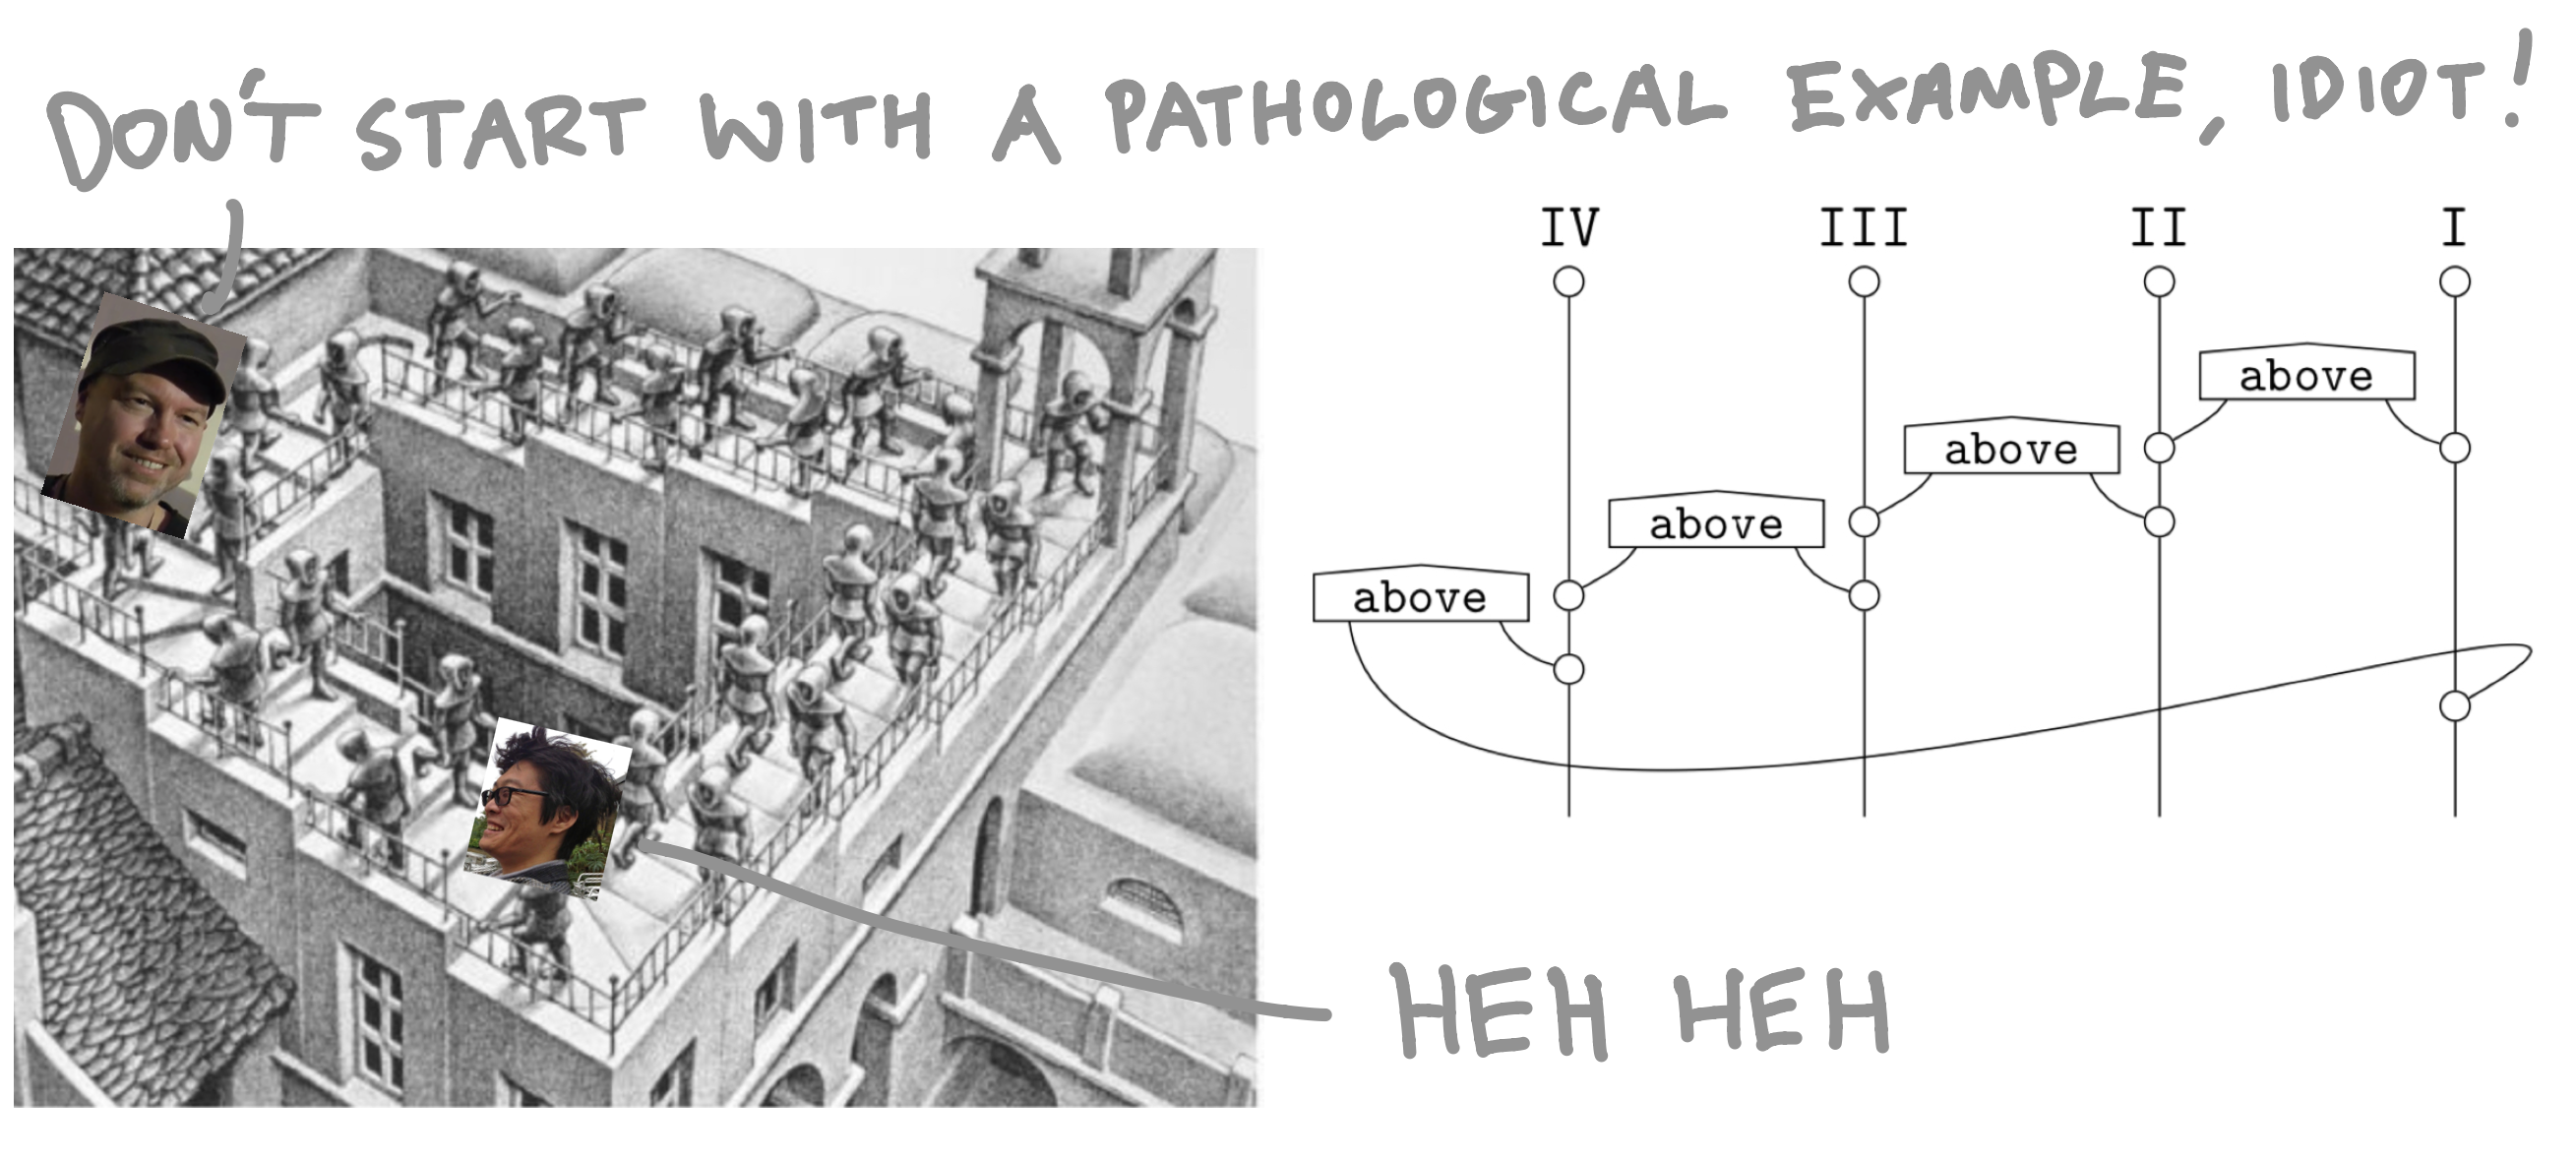
\includegraphics{figures/cartoons/space1}}
\caption{We wrote up the story about spaces in \bR CITE \e, the spiritual successor to \emph{interacting conceptual spaces I}. We could formally calculate the meanings of sentences that used linguistic spatial relations, all using a simple and tactile diagrammatic calculus.}
\end{figure}

\begin{figure}[h!]
\centering
\scalebox{1}{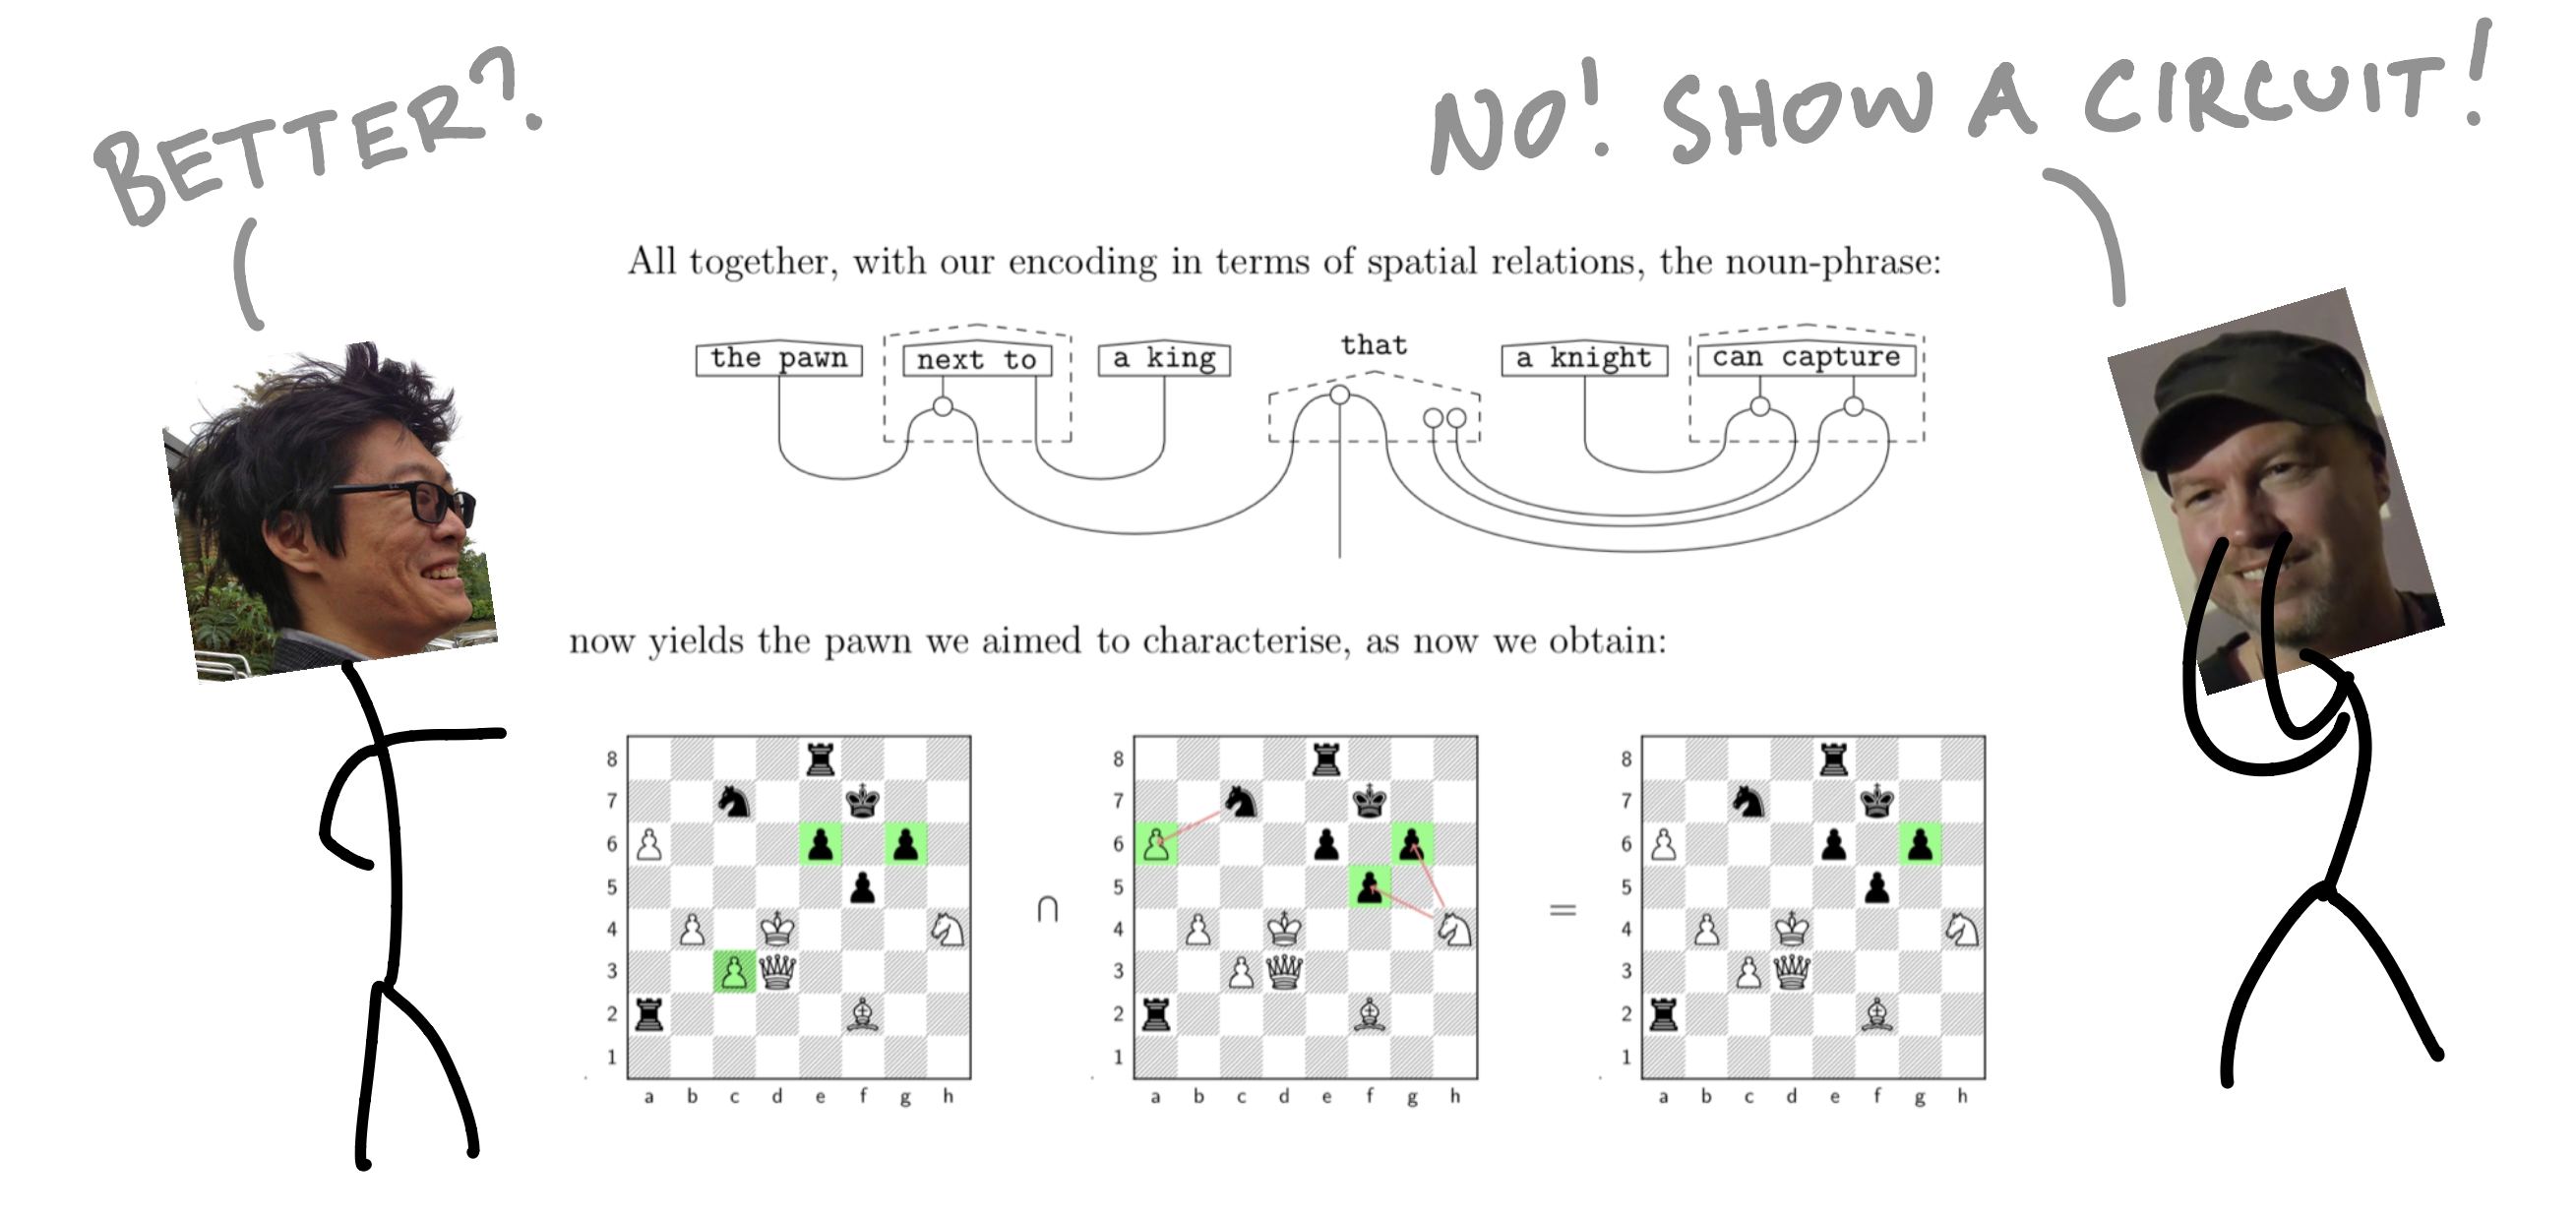
\includegraphics{figures/cartoons/space2}}
\end{figure}

\begin{figure}[h!]
\centering
\scalebox{1}{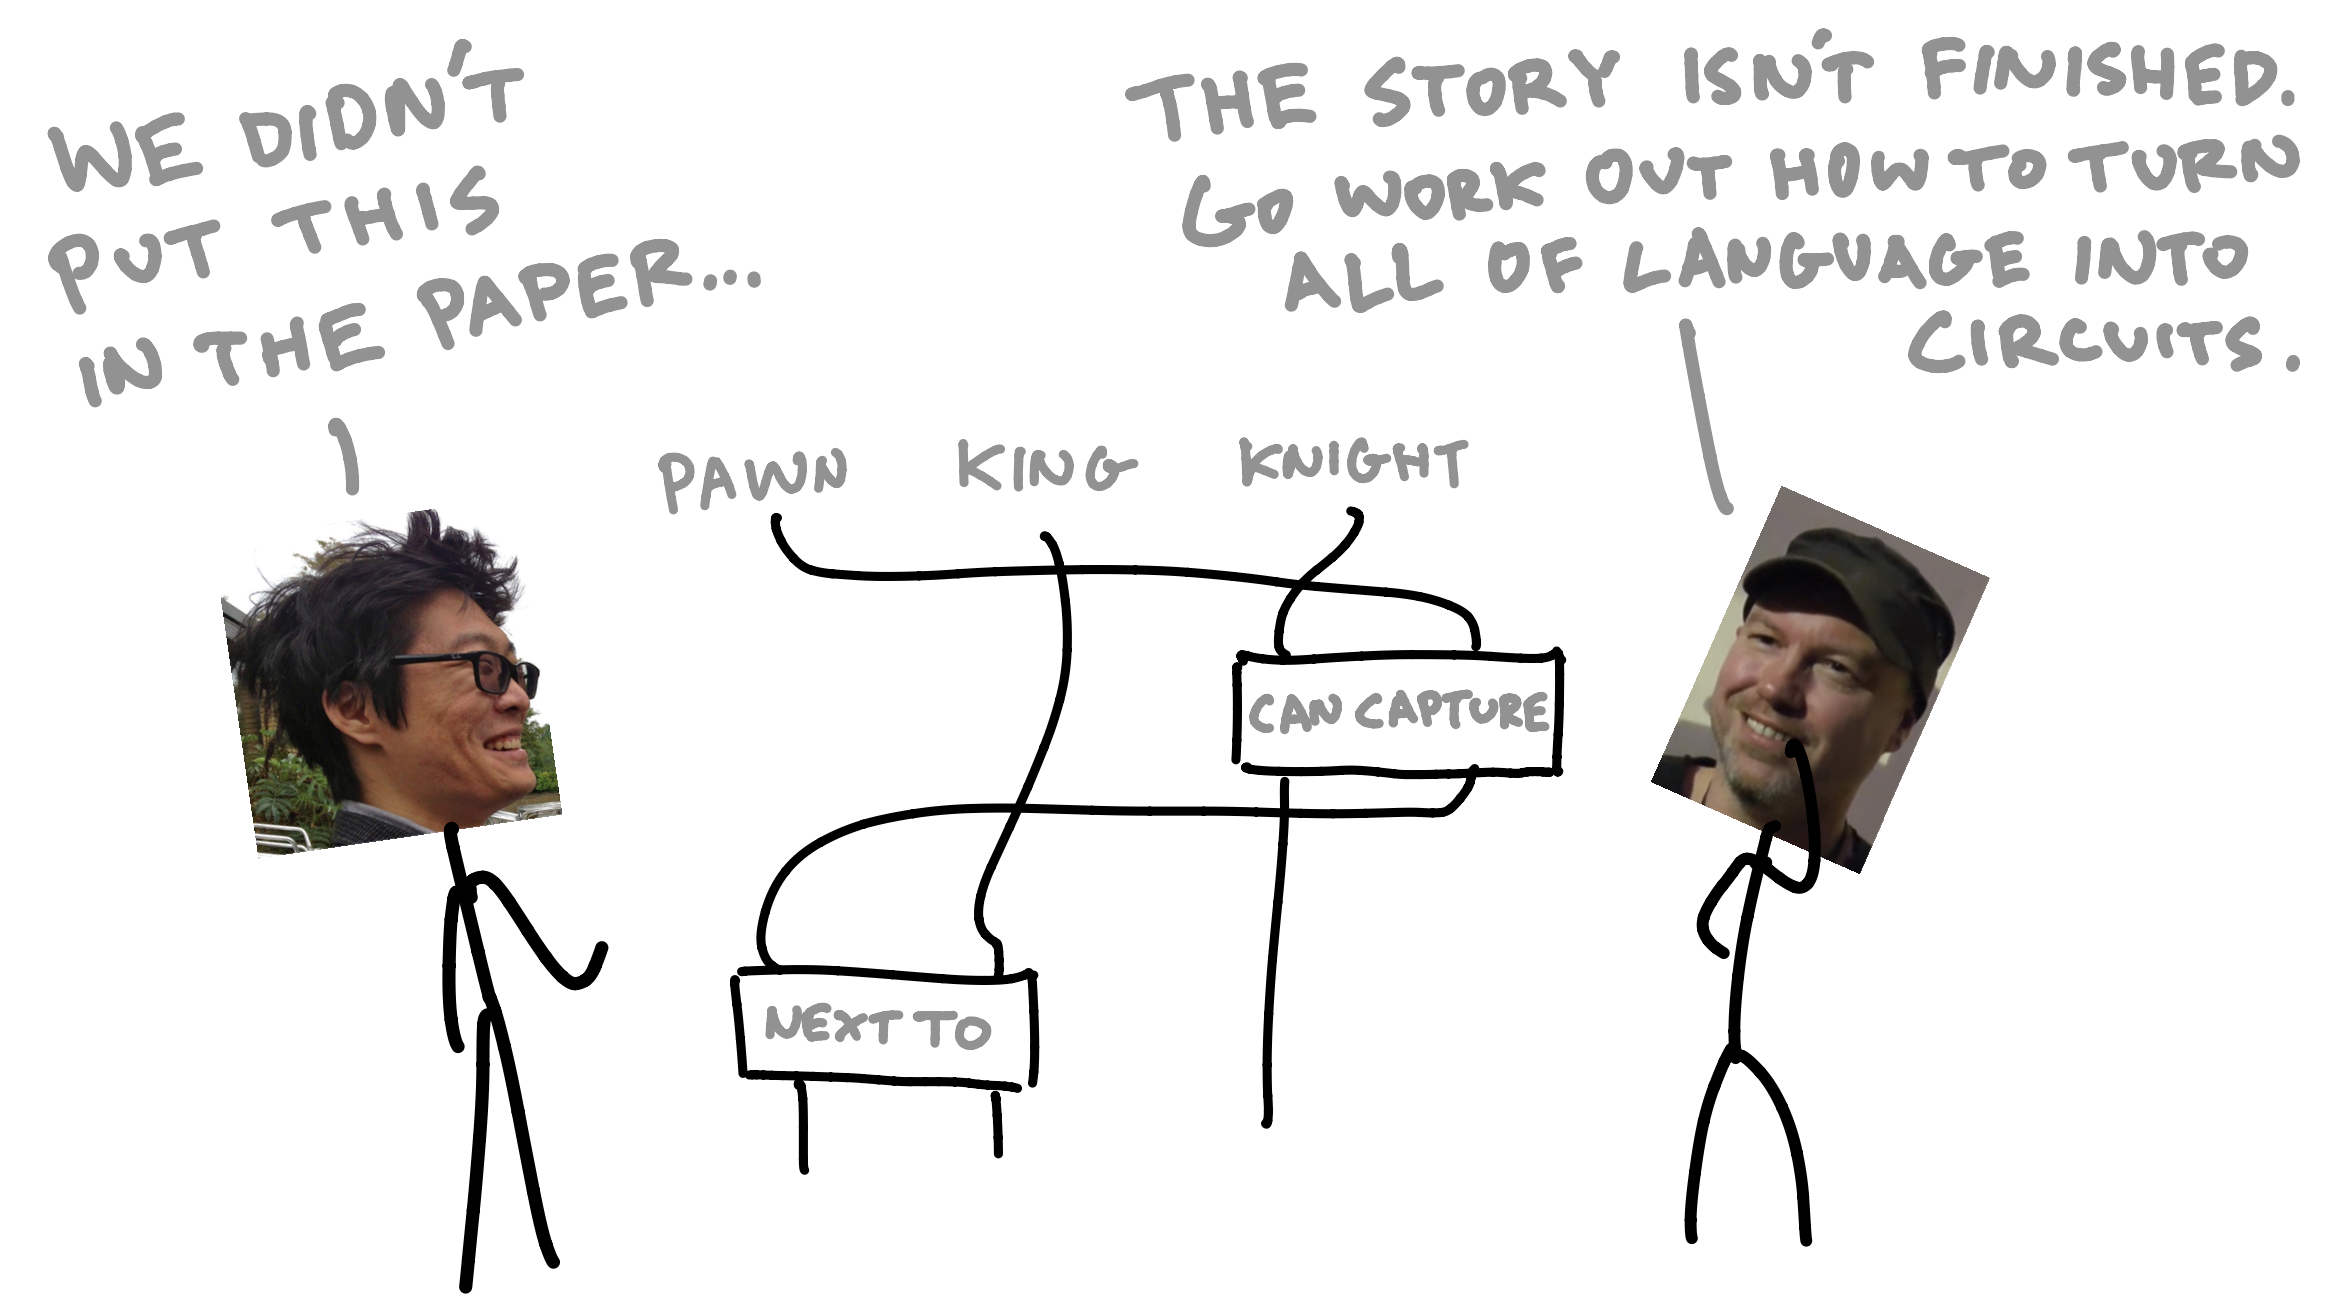
\includegraphics{figures/cartoons/space3}}
\caption{The paper on spatial relations actually came very late, because I was busy with Bob's ludicrous request to go turn "all of language" into circuits. I bitched and moaned about how I wasn't a linguist and how it was an impossible task, but I was in too deep to back out.}
\end{figure}

\begin{figure}[h!]
\centering
\scalebox{1}{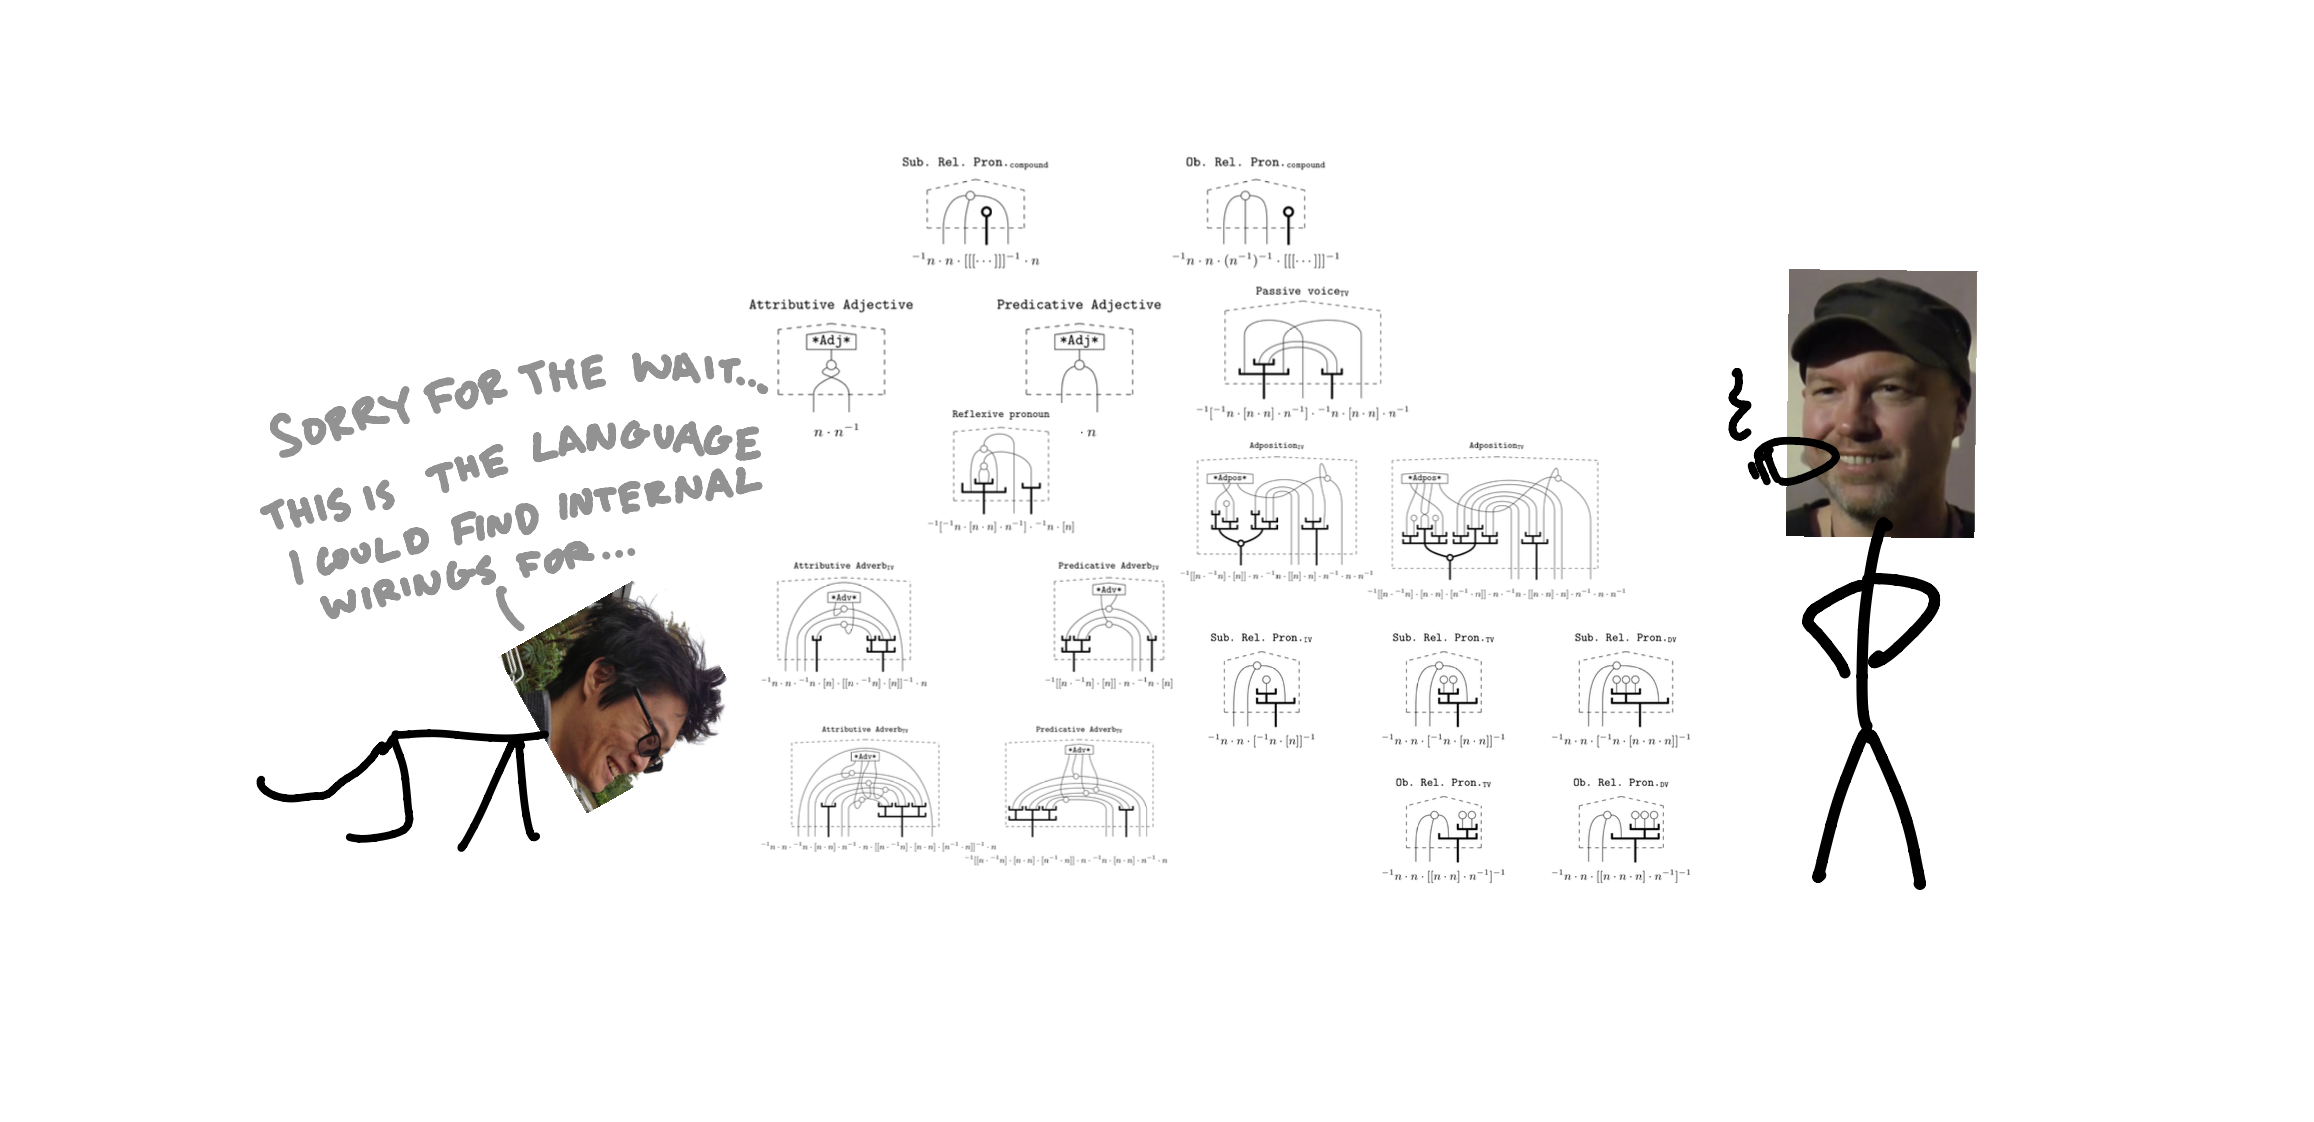
\includegraphics{figures/cartoons/pregroup1}}
\caption{I suppose the nice thing about aiming for the moon is that even failure might mean you leave orbit. So I settled for what I thought was a sensible fragment of English, for which I devised internal wirings and an algorithm that transformed pregroup diagrams with the internal wirings into circuit form. Many tiring diagrams later, I presented my results in the first draft of "distilling text into circuits".}
\end{figure}

\begin{figure}[h!]
\centering
\scalebox{1}{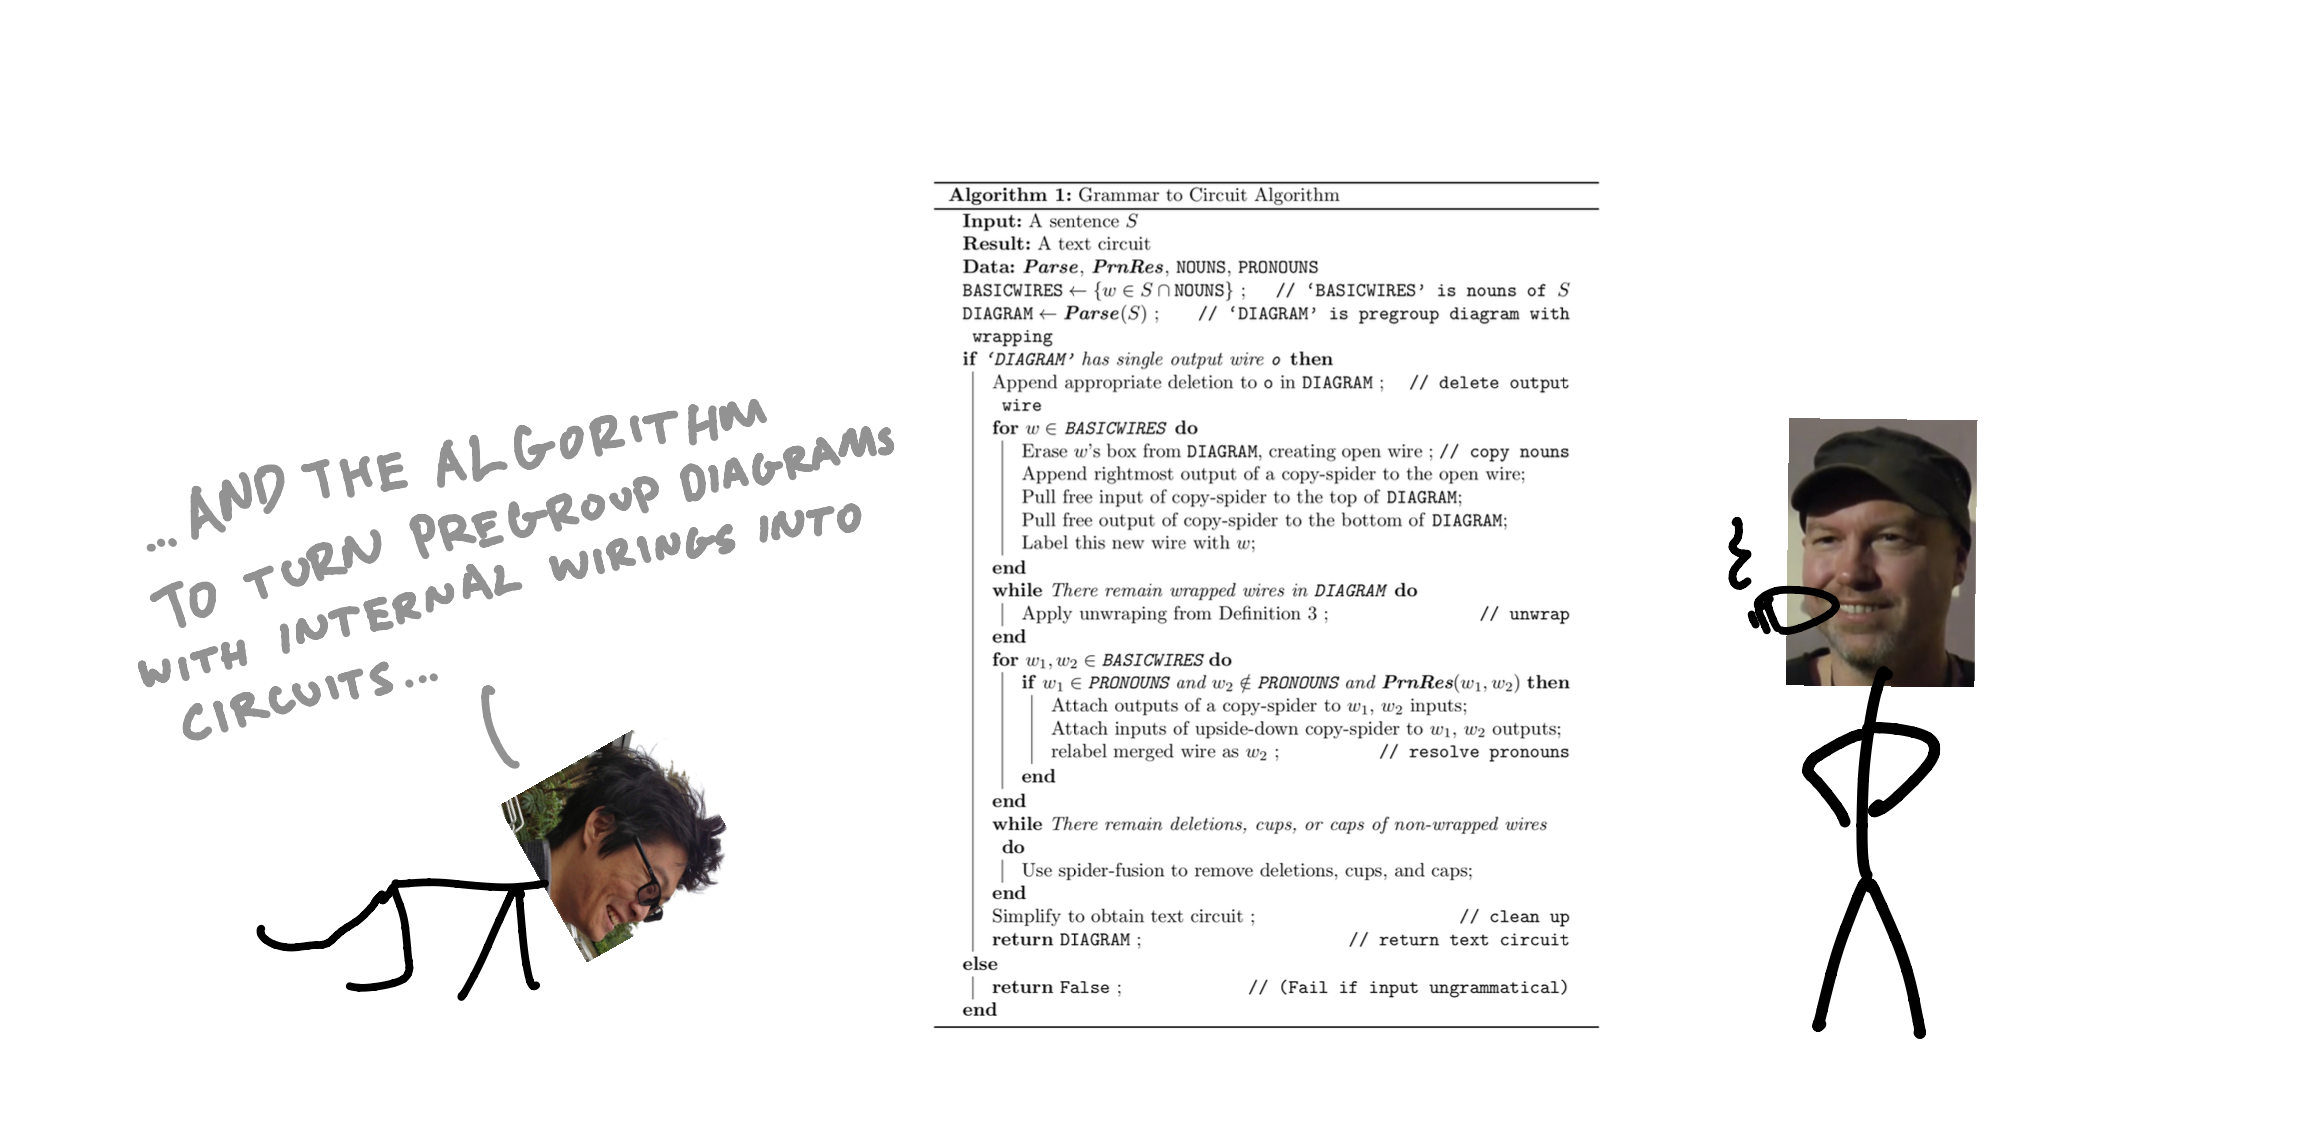
\includegraphics{figures/cartoons/pregroup2}}
\end{figure}

\begin{figure}[h!]
\centering
\scalebox{1}{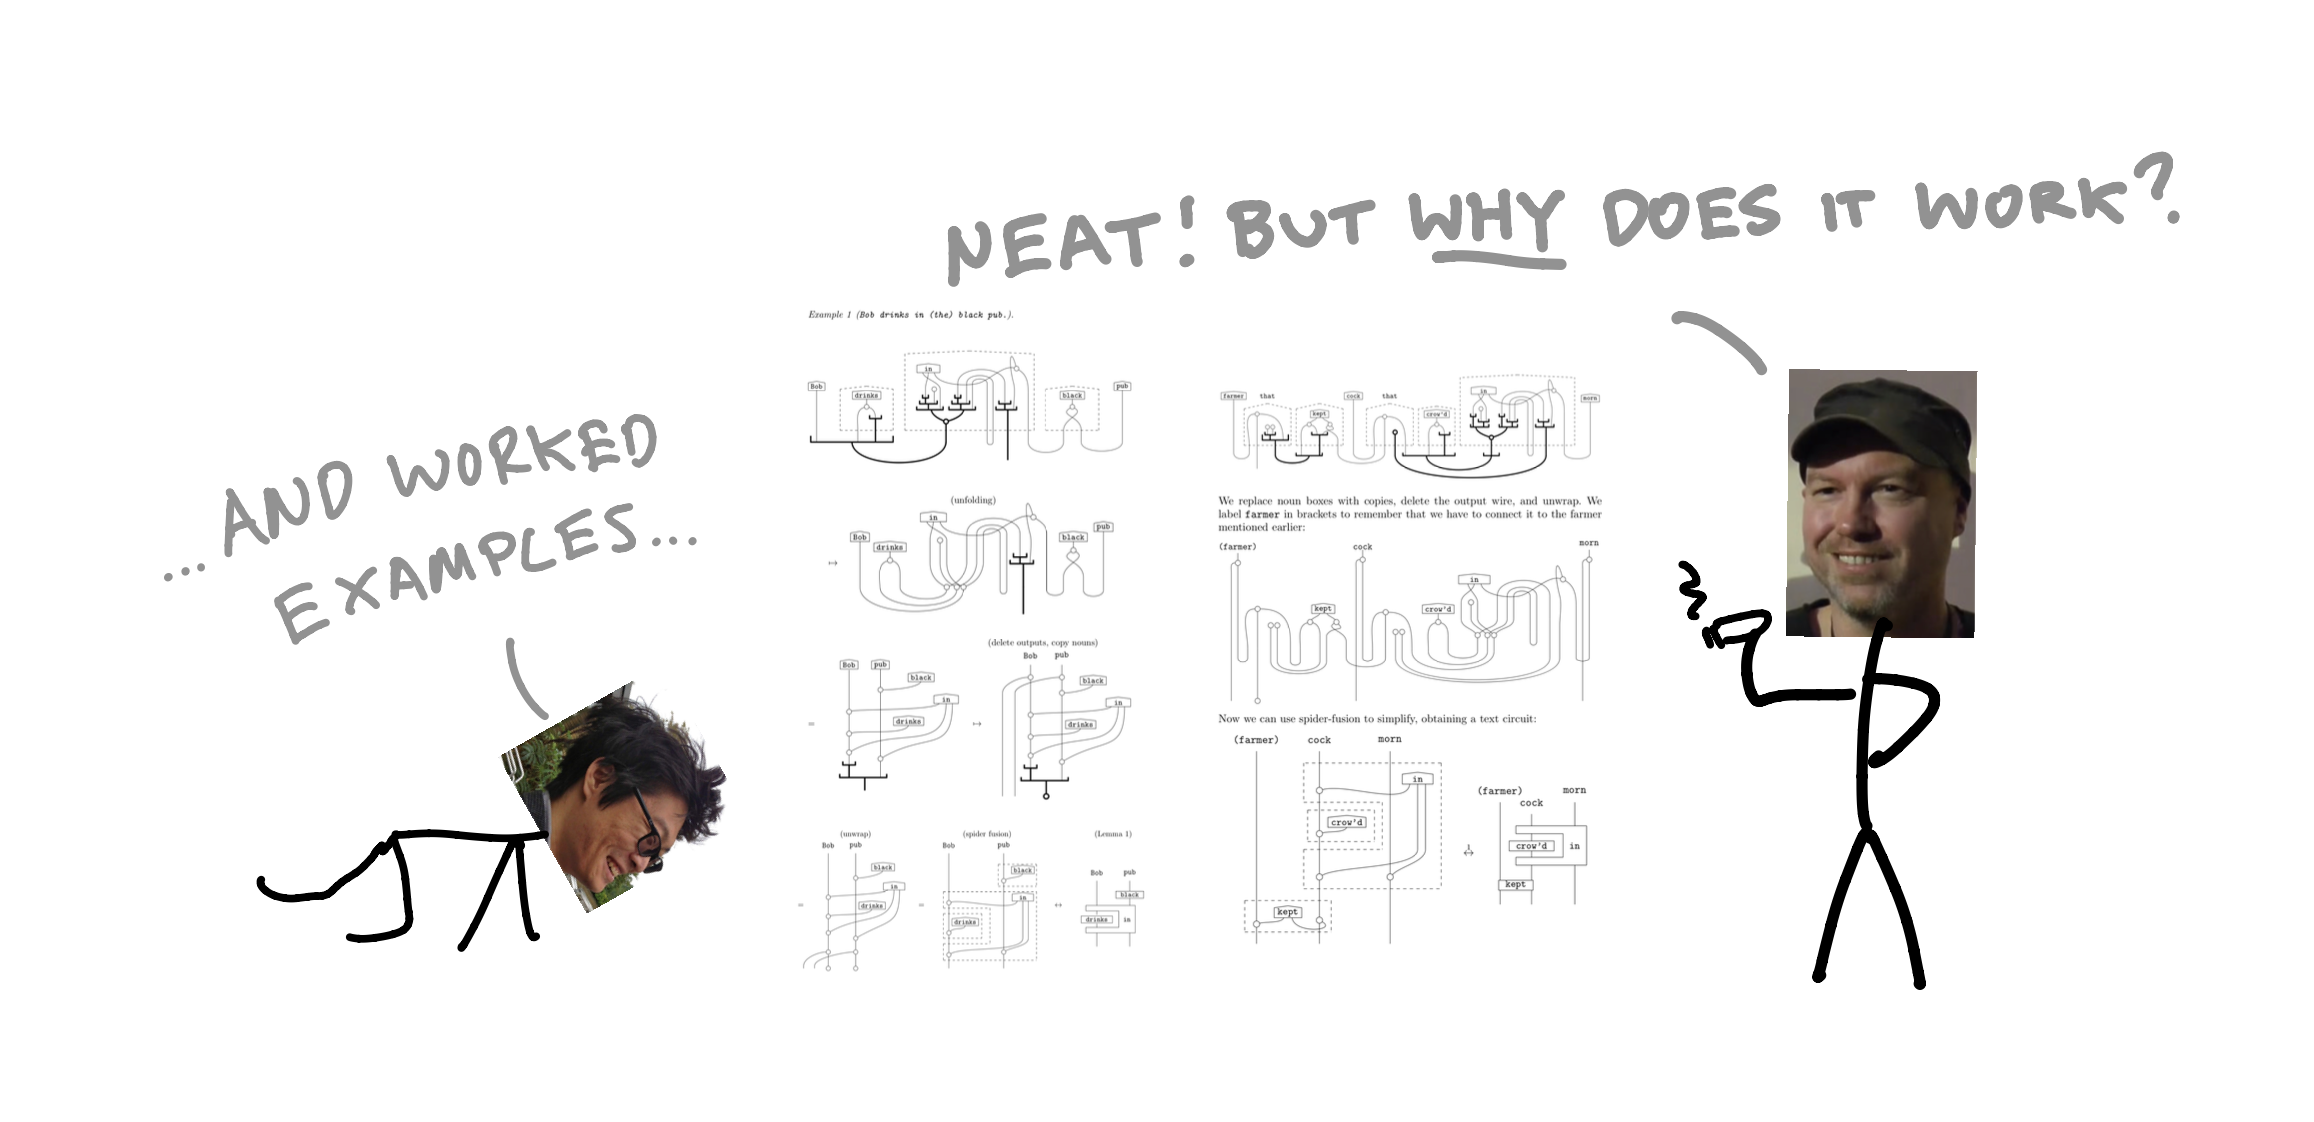
\includegraphics{figures/cartoons/pregroup3}}
\end{figure}

\begin{figure}[h!]
\centering
\scalebox{1}{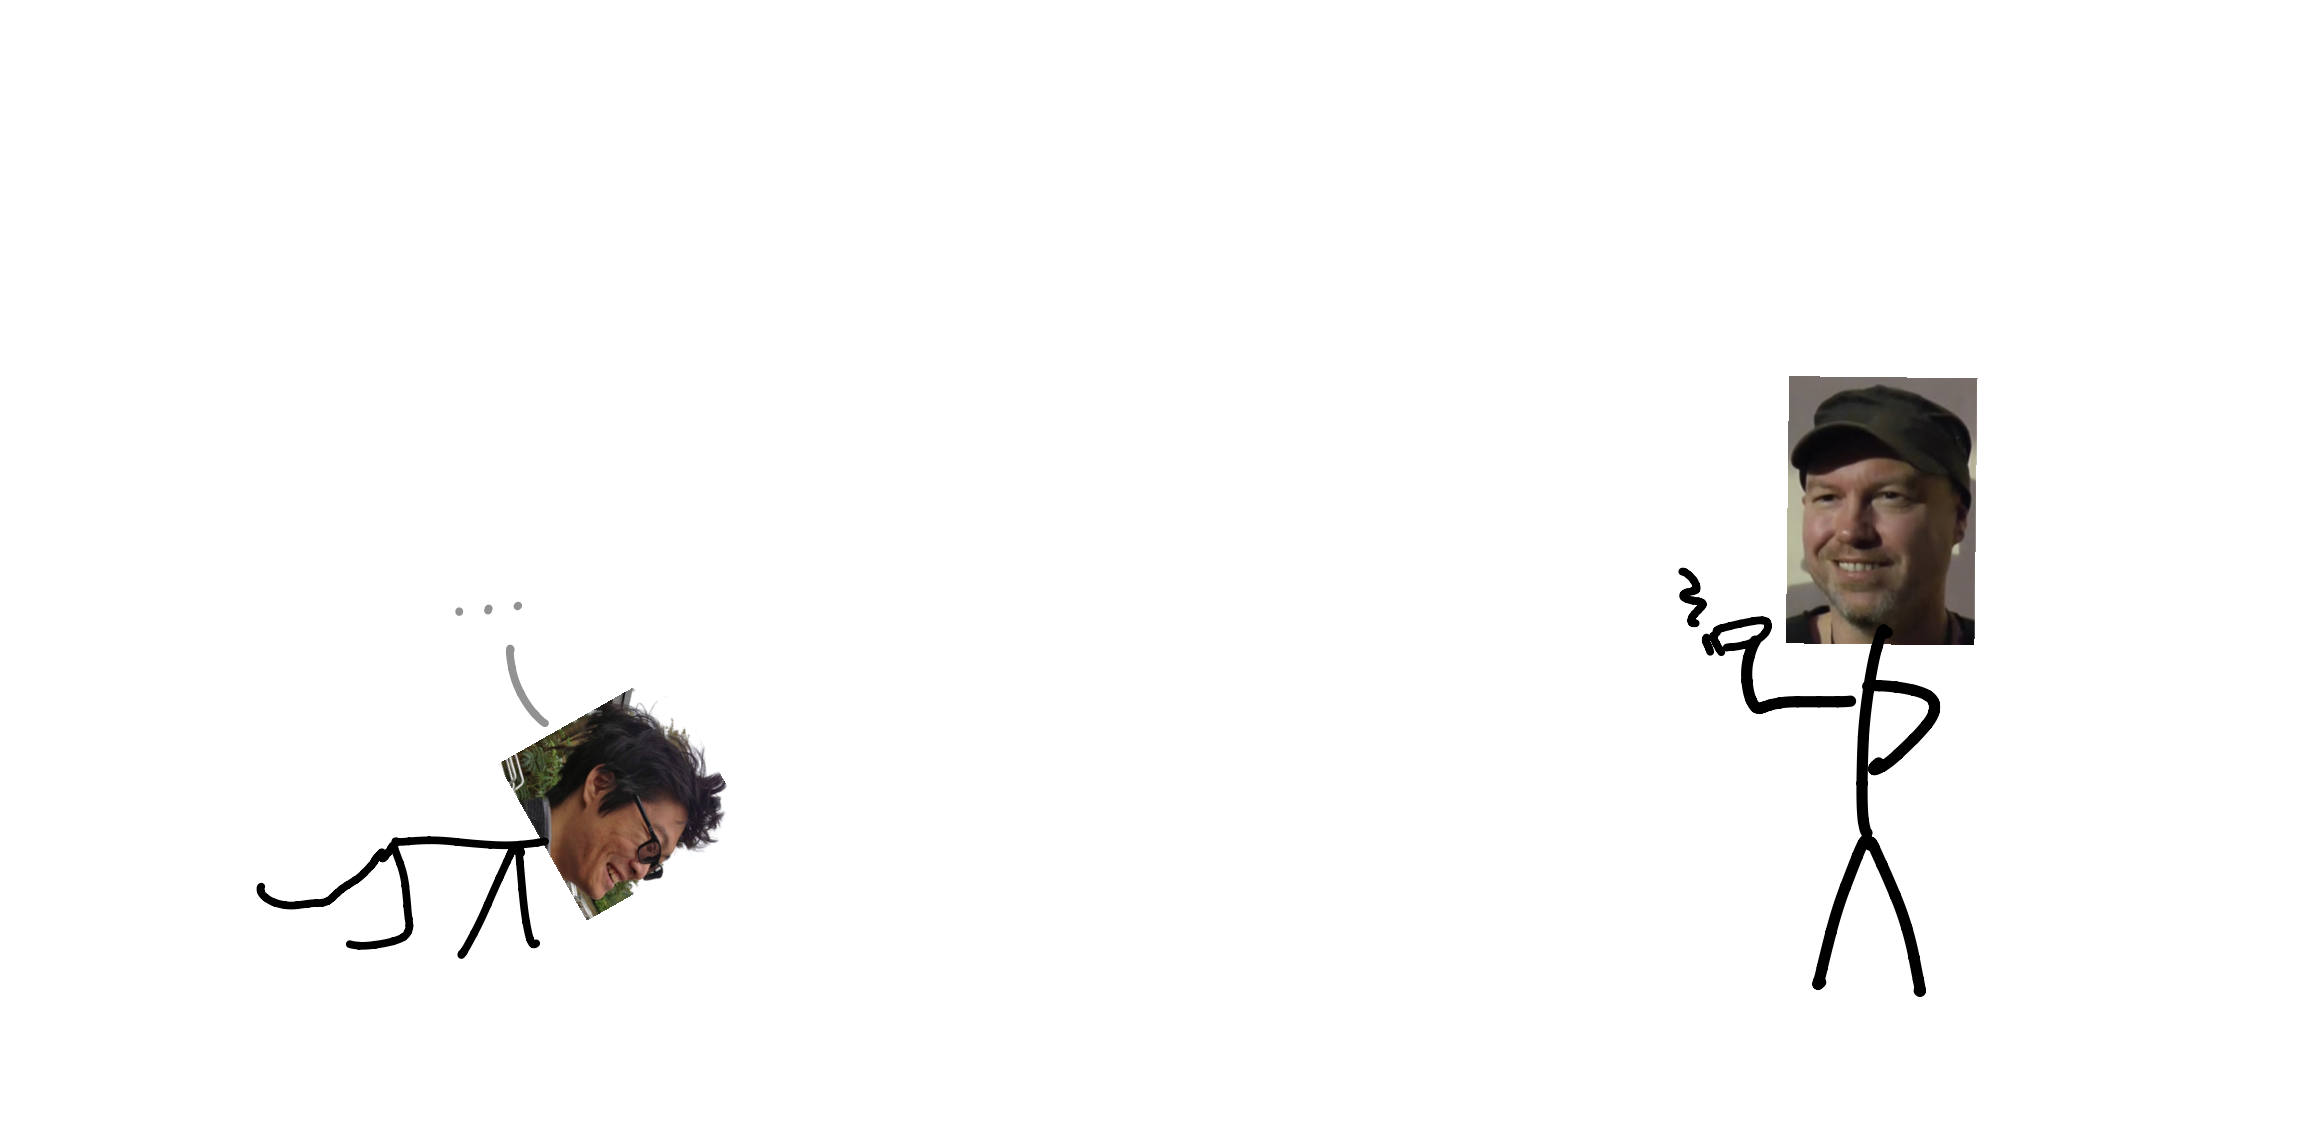
\includegraphics{figures/cartoons/pregroup4}}
\caption{Bob had a good point. Everything worked, but we had no understanding as to why, and accordingly, whether or not it would all break. At this point in time, Jonathon Liu, a masters' student I tutored during COVID, had committed the grave error of thinking diagrams were cool, and was now hanging out with me and Bob. After understanding the procedure, Jono independently devised the same arcane internal wirings as I had, but neither of us could explain how we did it. So we had evidence of an underlying governing structure that was coherent but inarticulable.}
\end{figure}

\begin{figure}[h!]
\centering
\scalebox{1}{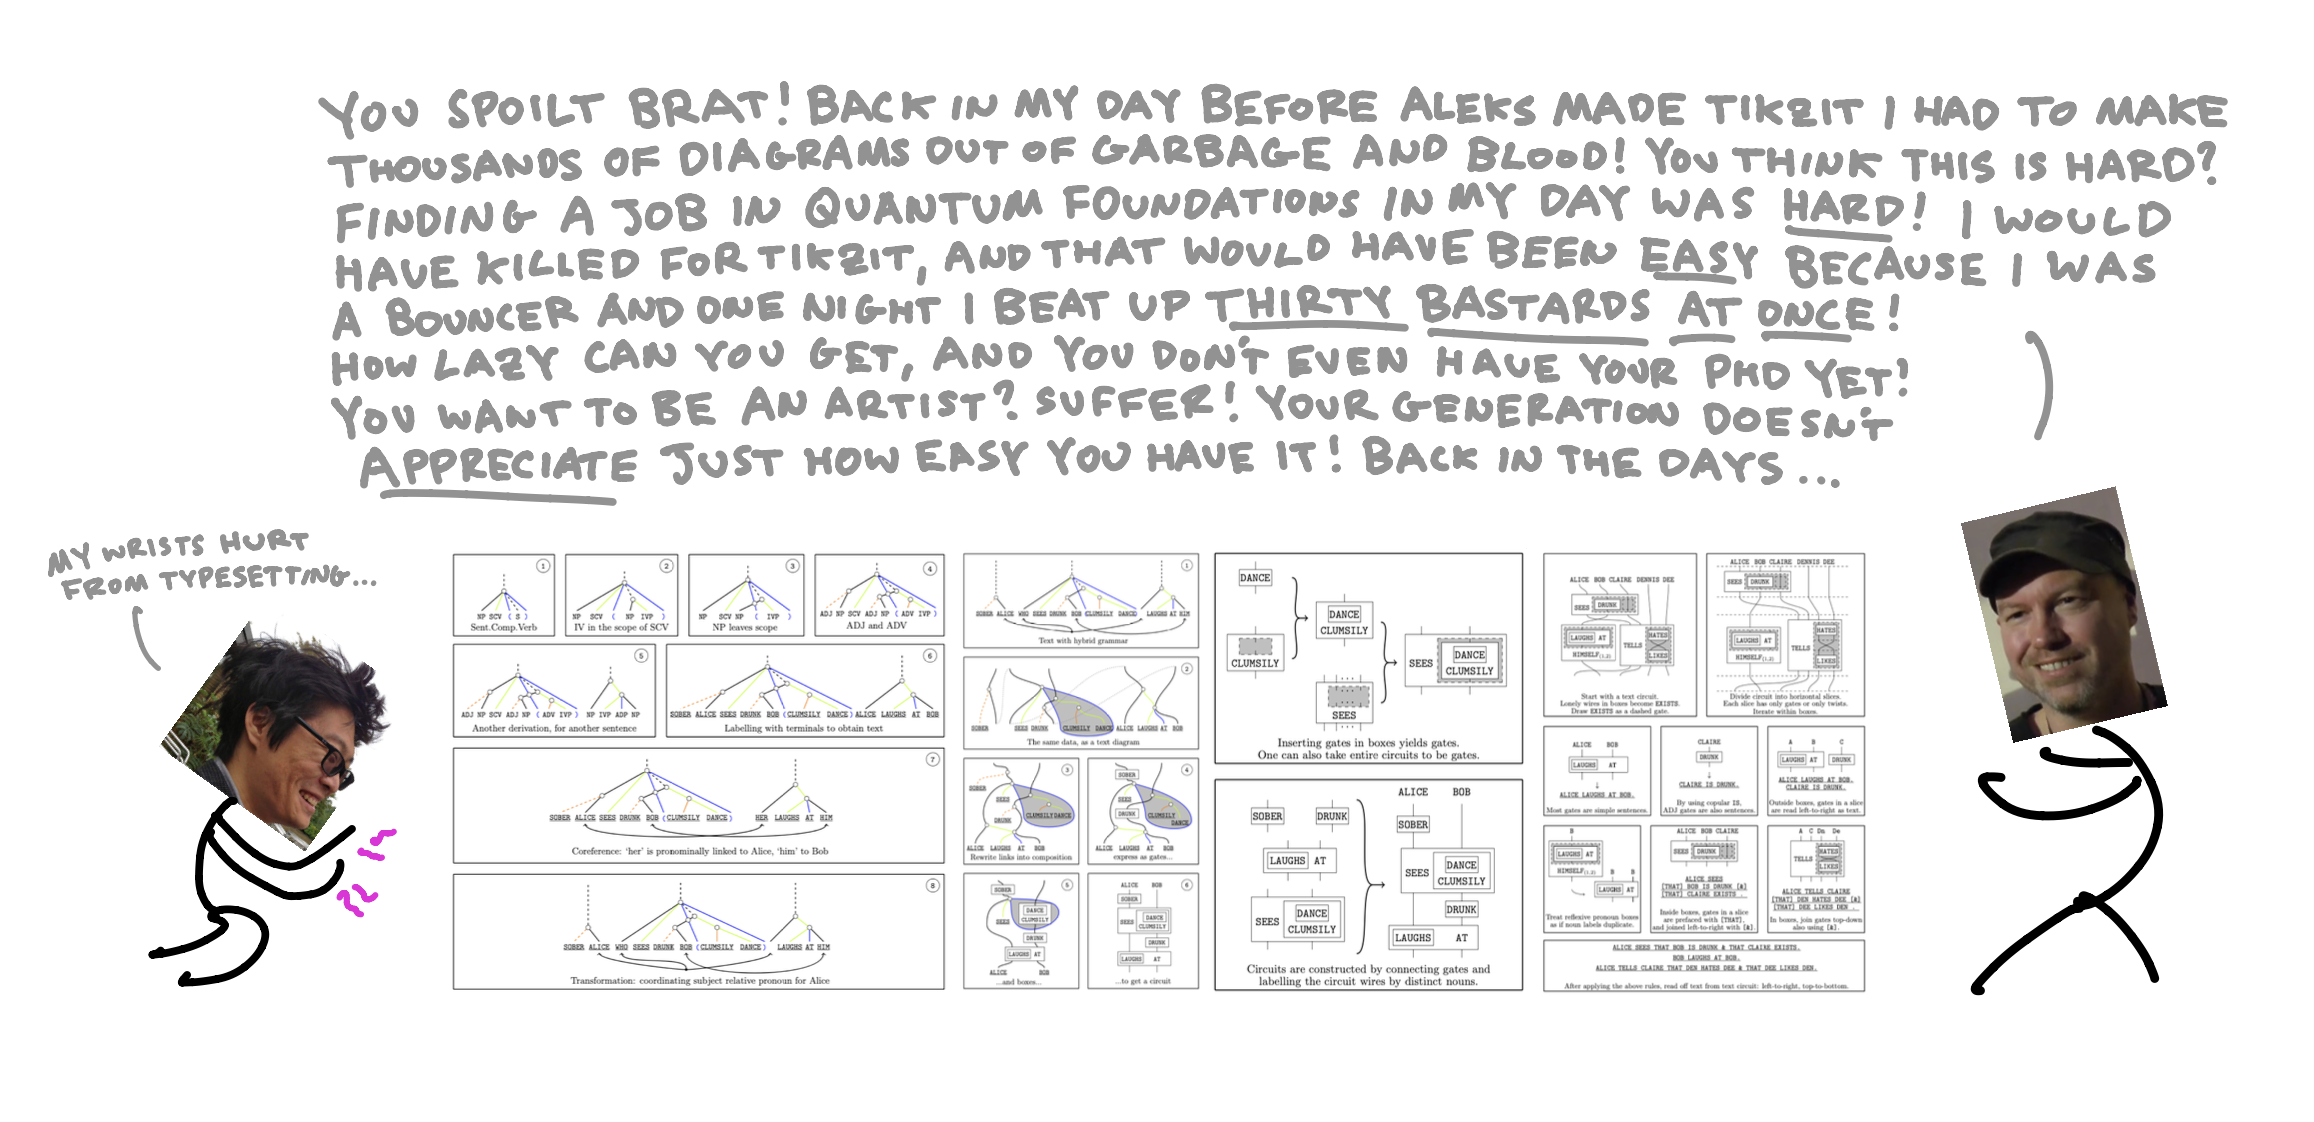
\includegraphics{figures/cartoons/bigpaper1}}
\caption{I realised that our intuitions were coming from an implicit productive grammar, rather than a parsing one, and that the path of least resistance for obtaining formal guarantees for the language-to-circuit procedure was to just handcraft a generative grammar for the fragment of language we were interested in. This meant scrapping everything in the first draft and starting again from scratch. Bob always had a word of gentle encouragement, giving me the motivation to persevere.\\

So now we had two ways to obtain text circuits. One from pregroups (which Jono had extended the technique for to CCGs in his master's thesis \bR CITE \e), and one from handcrafted productive grammars. Then came time for me to write my thesis, and there were three salient questions I wanted to address.\\
Firstly, what are internal wirings?\\
Secondly, how do text circuits relate to other generative grammars?\\
Thirdly, what are text circuits good for?\\
These questions are now what the rest of the thesis seeks to answer.
}
\end{figure}



\bibliographystyle{alpha}
\bibliography{thesis_intro}





\end{document}